\documentclass[12pt,a4paper]{article}

\usepackage[utf8]{inputenc}
\usepackage[T1]{fontenc}
\usepackage[spanish]{babel}
\usepackage{amsmath, amssymb}
\usepackage{graphicx}
\usepackage{geometry}
\usepackage{hyperref}

\geometry{margin=2.5cm}

\title{Prácticas guiadas - Apache NiFi}
\author{Francisco Javier Porta Borge}
\date{\today}

\begin{document}

\maketitle

\tableofcontents




\section{Practica 1 - Instalación y configuración de Lubuntu 26.04.1}
\subsection{Instalación de la ISO de Lubuntu}
\begin{figure}[ht]
    \centering
    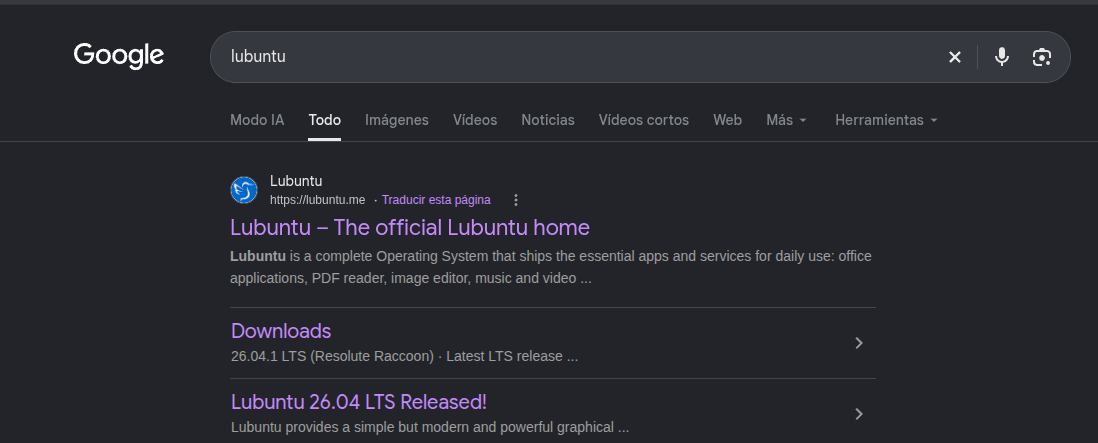
\includegraphics[width=0.8\textwidth]{1.png}
    \caption{Imagen 1}
    \label{fig:imagen1}
\end{figure}

\begin{figure}[ht]
    \centering
    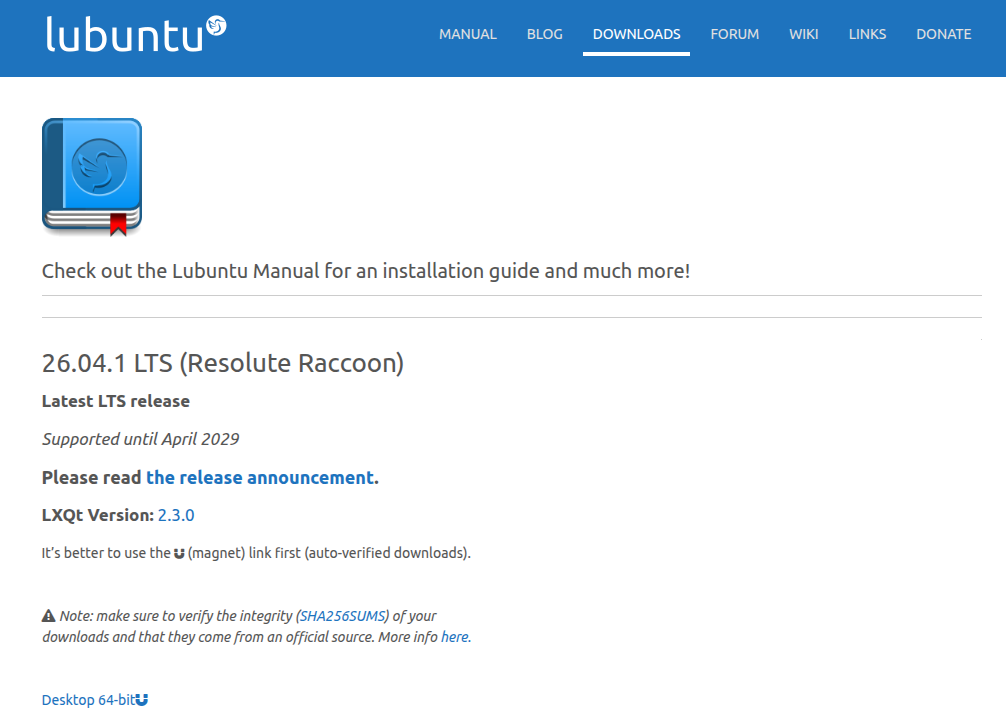
\includegraphics[width=0.8\textwidth]{2.png}
    \caption{Imagen 2}
    \label{fig:imagen2}
\end{figure}

\subsection{Creación de la maquina virtual}
\begin{figure}[ht]
    \centering
    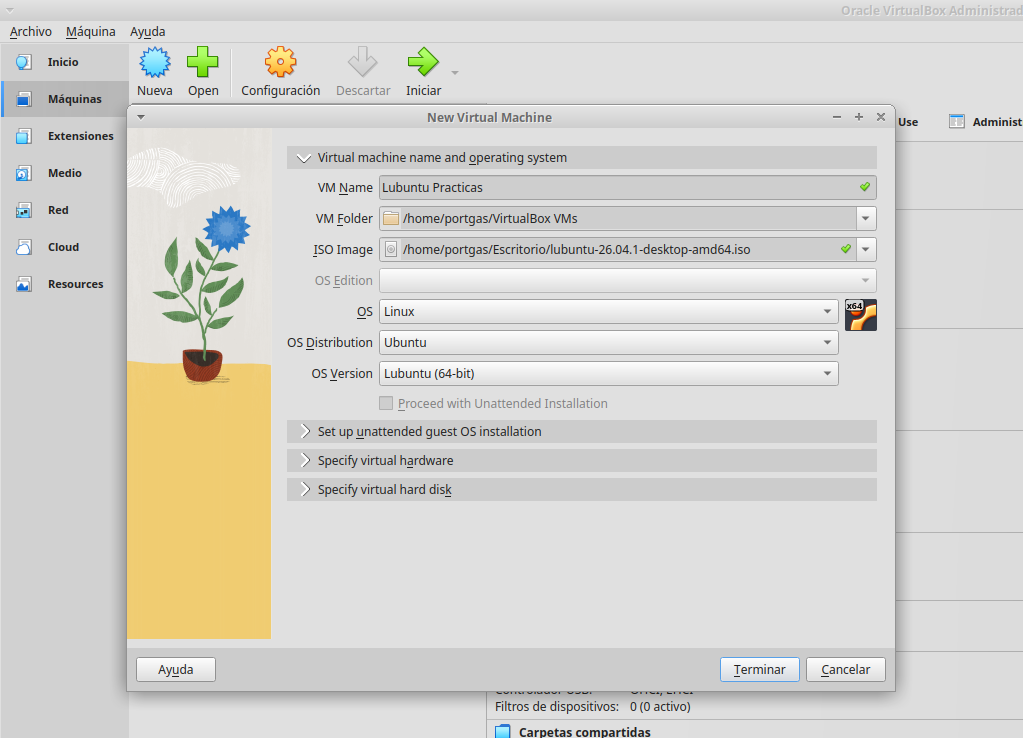
\includegraphics[width=0.8\textwidth]{3.png}
    \caption{Imagen 1}
    \label{fig:imagen1}
\end{figure}
\begin{figure}[ht]
    \centering
    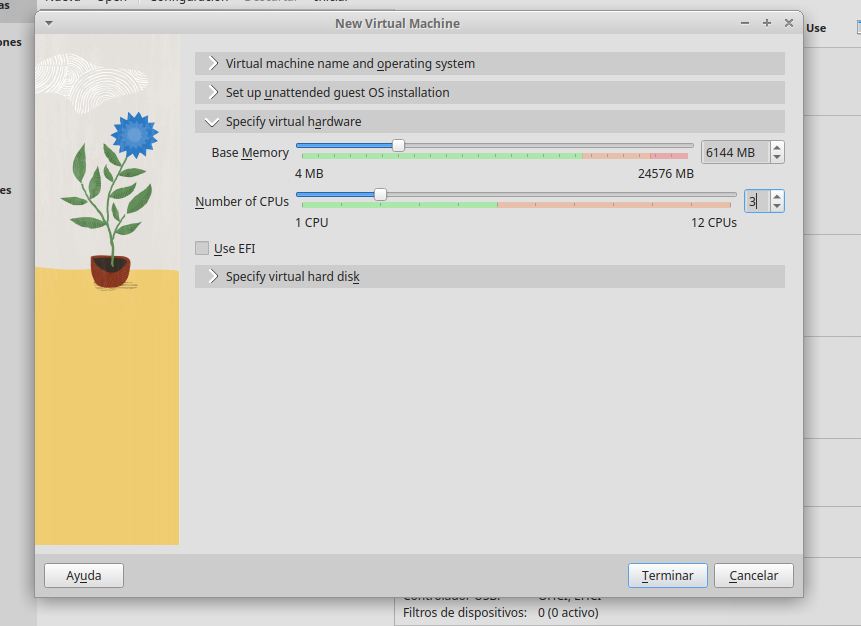
\includegraphics[width=0.8\textwidth]{4.png}
    \caption{Imagen 1}
    \label{fig:imagen1}
\end{figure}
\begin{figure}[ht]
    \centering
    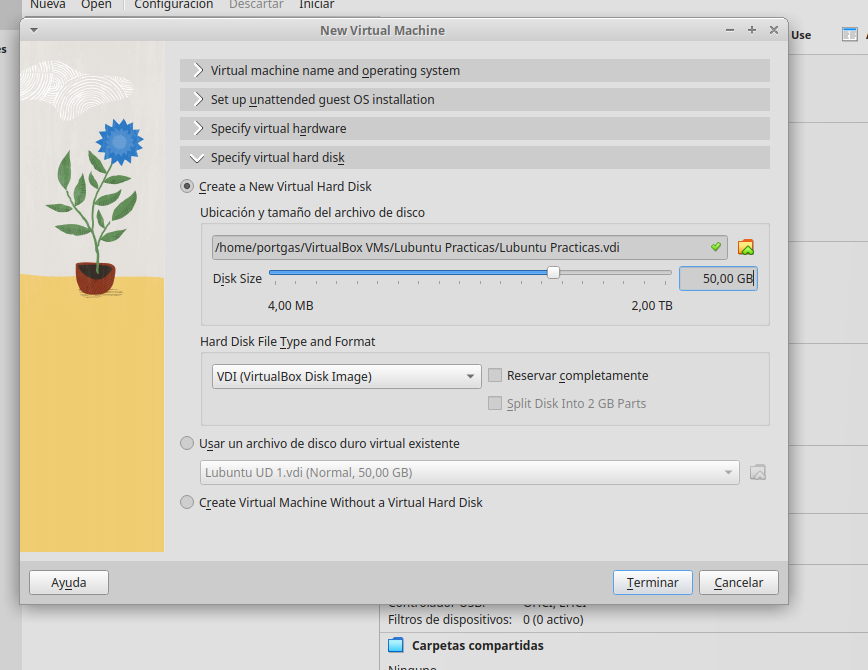
\includegraphics[width=0.8\textwidth]{5.png}
    \caption{Imagen 1}
    \label{fig:imagen1}
\end{figure}
\begin{figure}[ht]
    \centering
    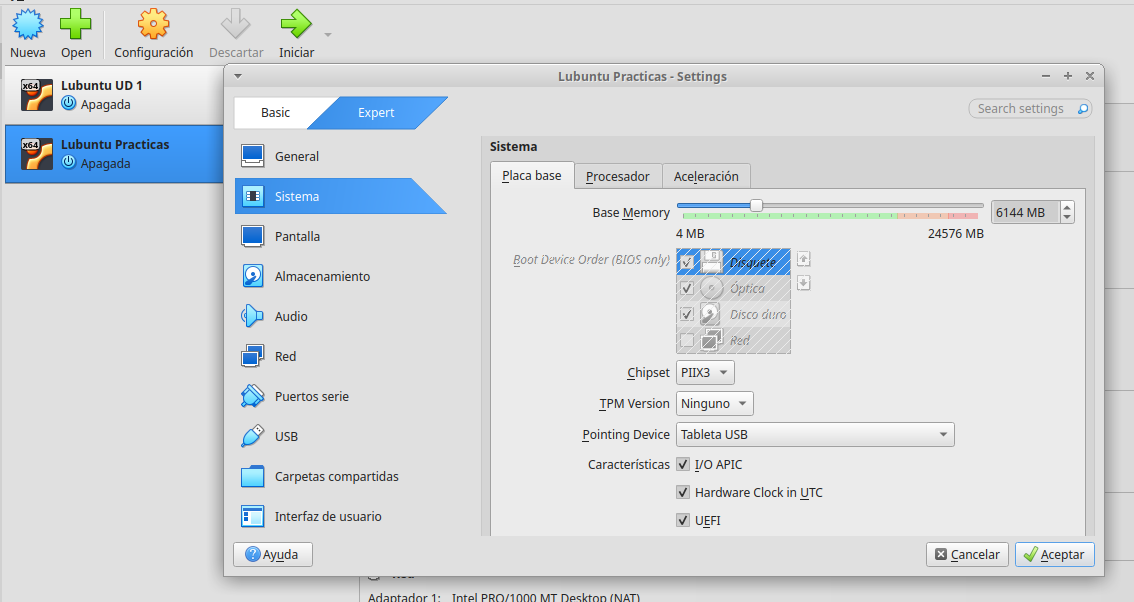
\includegraphics[width=0.8\textwidth]{6.png}
    \caption{Imagen 1}
    \label{fig:imagen1}
\end{figure}
\begin{figure}[ht]
    \centering
    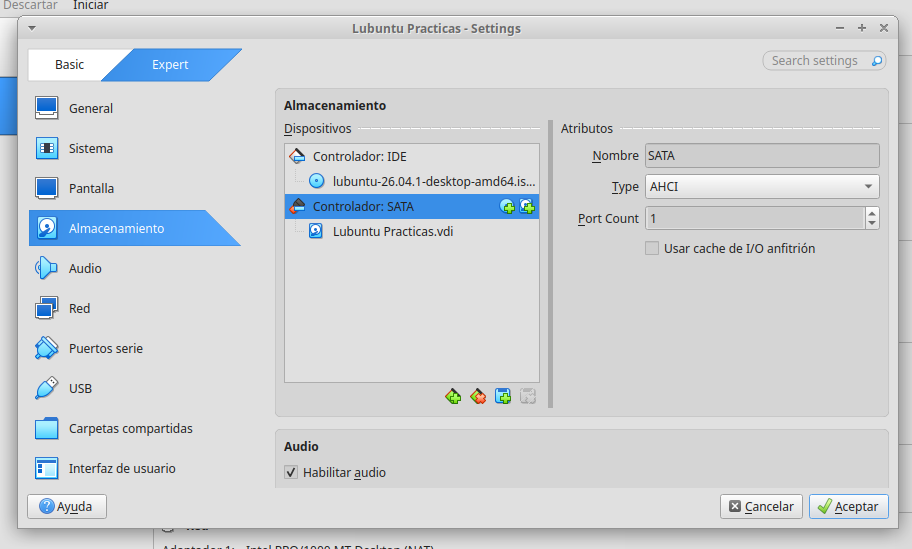
\includegraphics[width=0.8\textwidth]{7.png}
    \caption{Imagen 1}
    \label{fig:imagen1}
\end{figure}
\begin{figure}[ht]
    \centering
    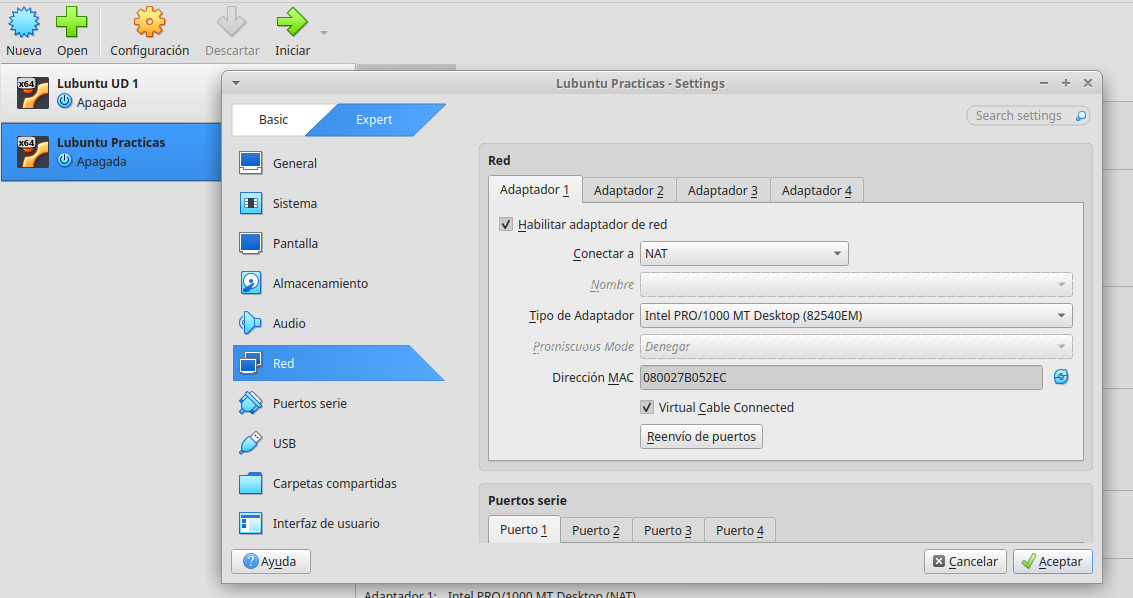
\includegraphics[width=0.8\textwidth]{8.png}
    \caption{Imagen 1}
    \label{fig:imagen1}
\end{figure}
\subsection{Proceso de instalación}
\begin{figure}[ht]
    \centering
    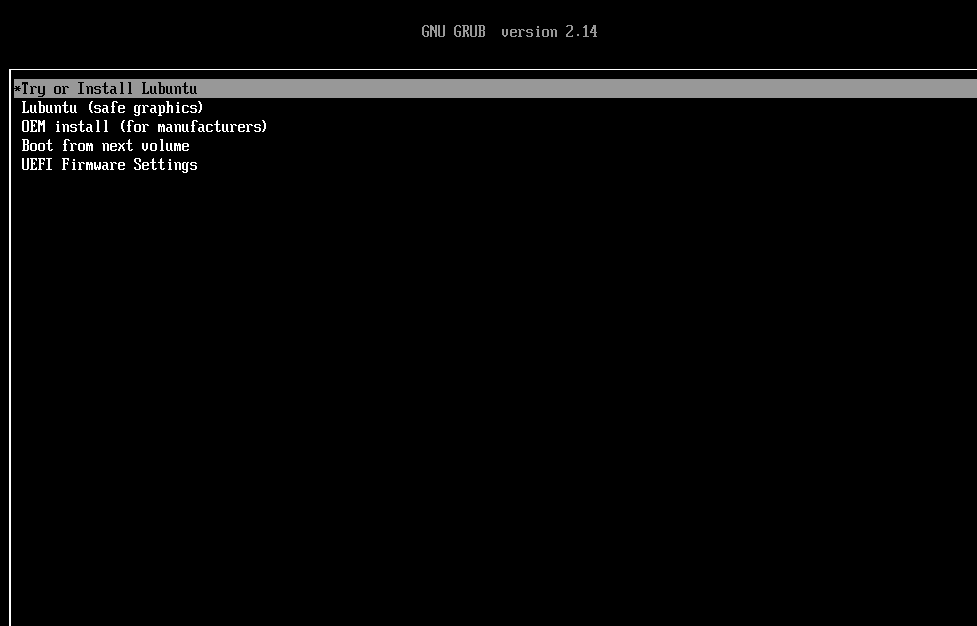
\includegraphics[width=0.8\textwidth]{9.png}
    \caption{Imagen 1}
    \label{fig:imagen1}
\end{figure}
\begin{figure}[ht]
    \centering
    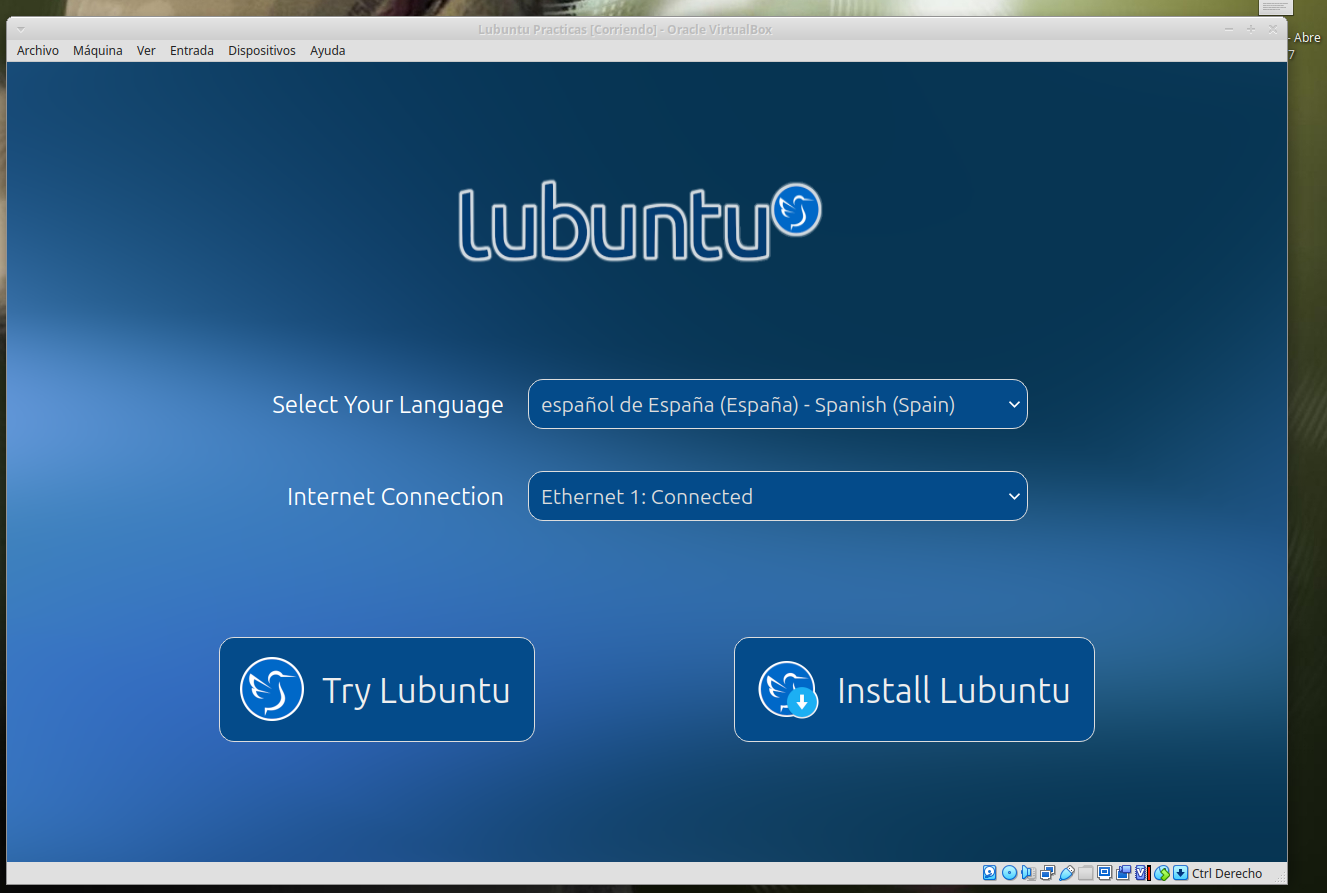
\includegraphics[width=0.8\textwidth]{10.png}
    \caption{Imagen 1}
    \label{fig:imagen1}
\end{figure}
\begin{figure}[ht]
    \centering
    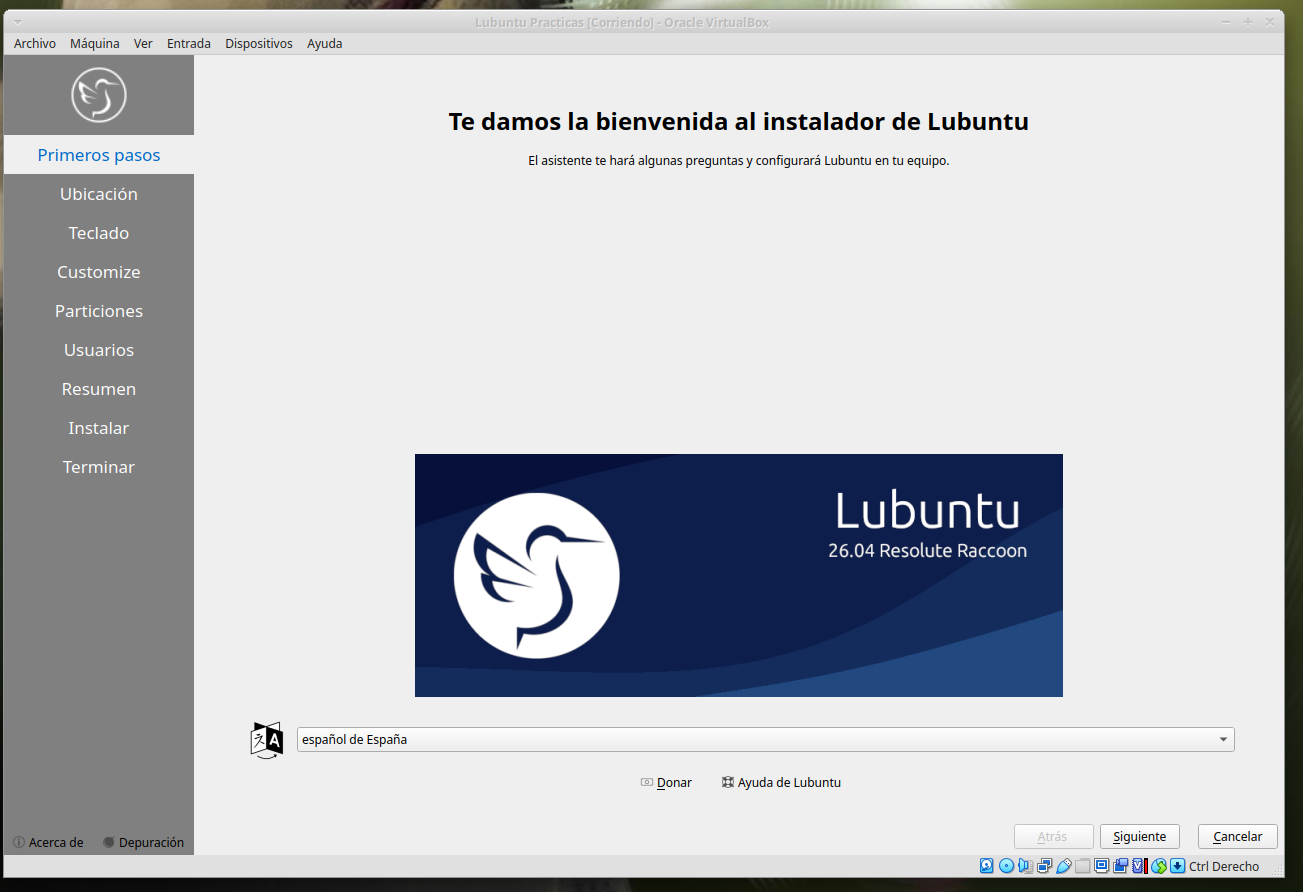
\includegraphics[width=0.8\textwidth]{11.png}
    \caption{Imagen 1}
    \label{fig:imagen1}
\end{figure}
\begin{figure}[ht]
    \centering
    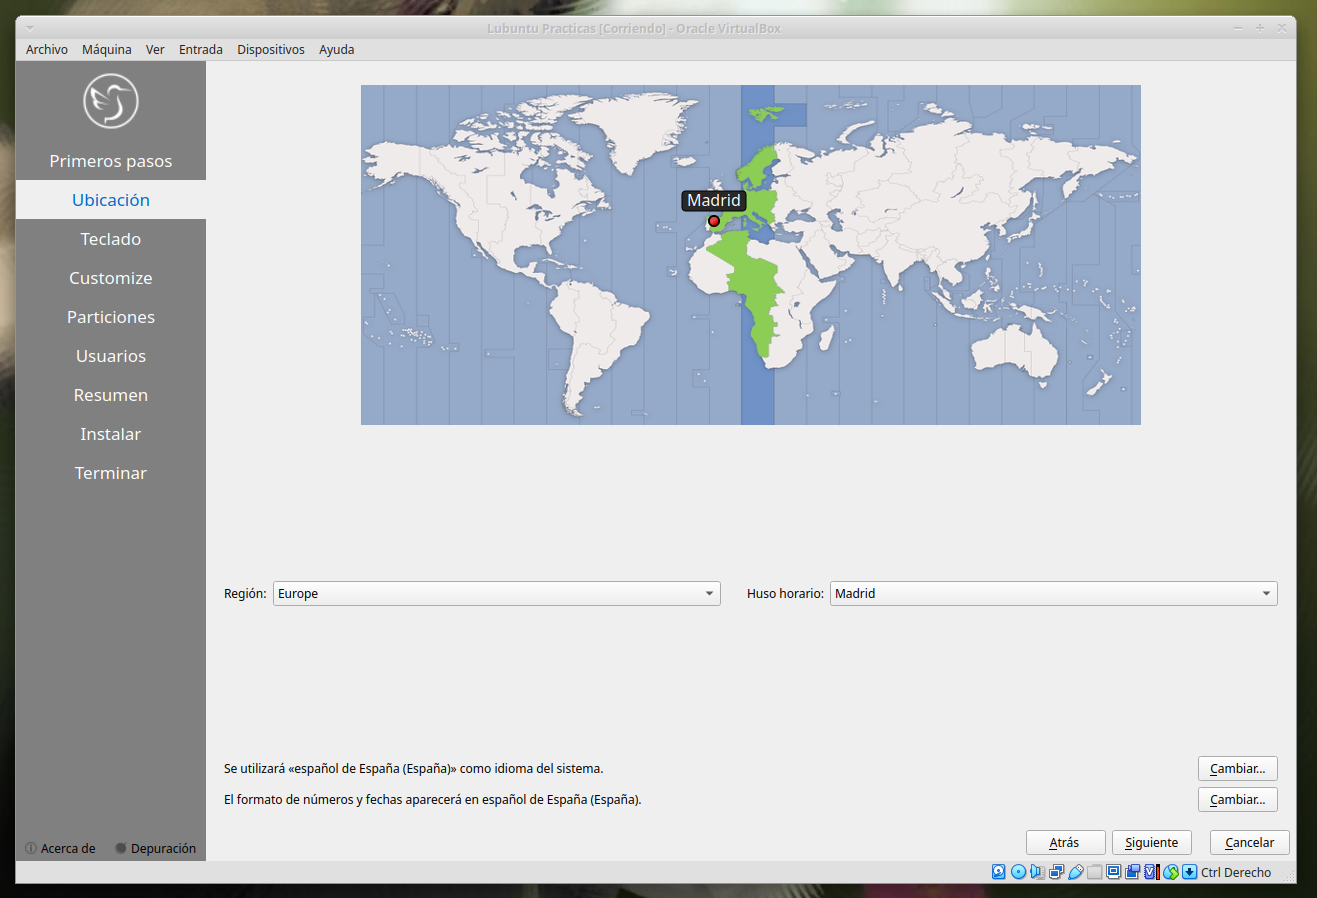
\includegraphics[width=0.8\textwidth]{12.png}
    \caption{Imagen 1}
    \label{fig:imagen1}
\end{figure}
\begin{figure}[ht]
    \centering
    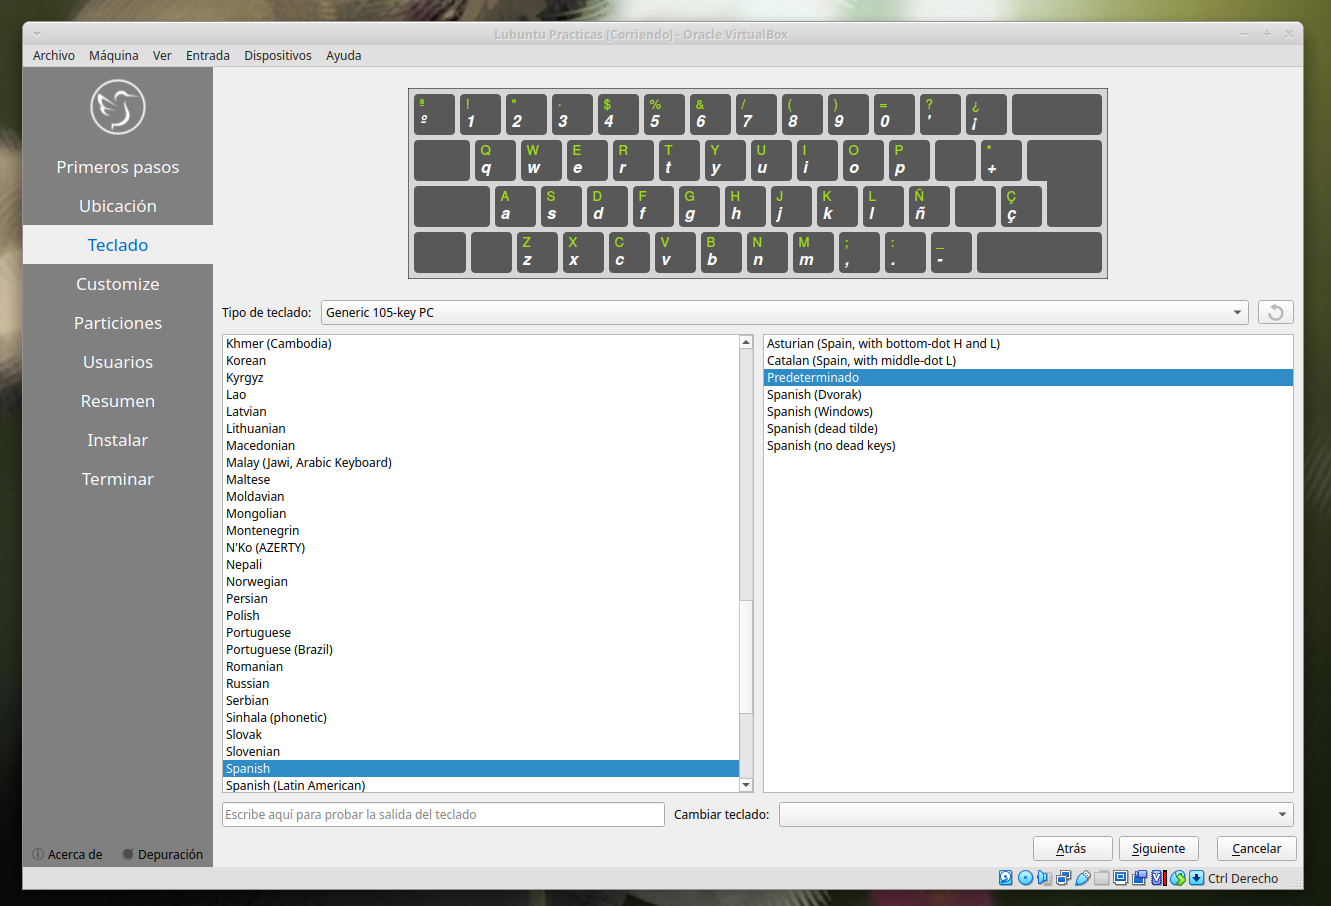
\includegraphics[width=0.8\textwidth]{13.png}
    \caption{Imagen 1}
    \label{fig:imagen1}
\end{figure}
\begin{figure}[ht]
    \centering
    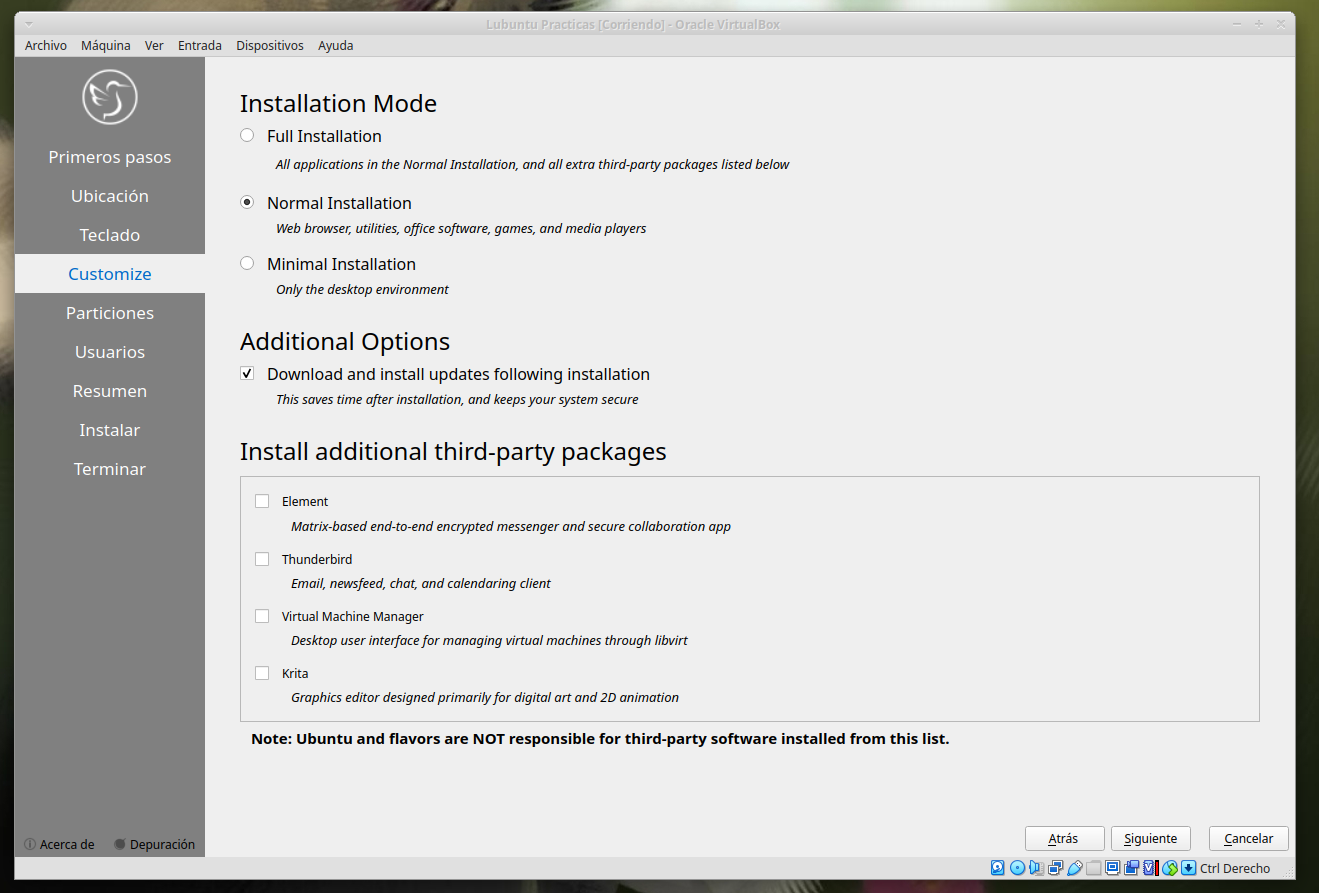
\includegraphics[width=0.8\textwidth]{14.png}
    \caption{Imagen 1}
    \label{fig:imagen1}
\end{figure}
\begin{figure}[ht]
    \centering
    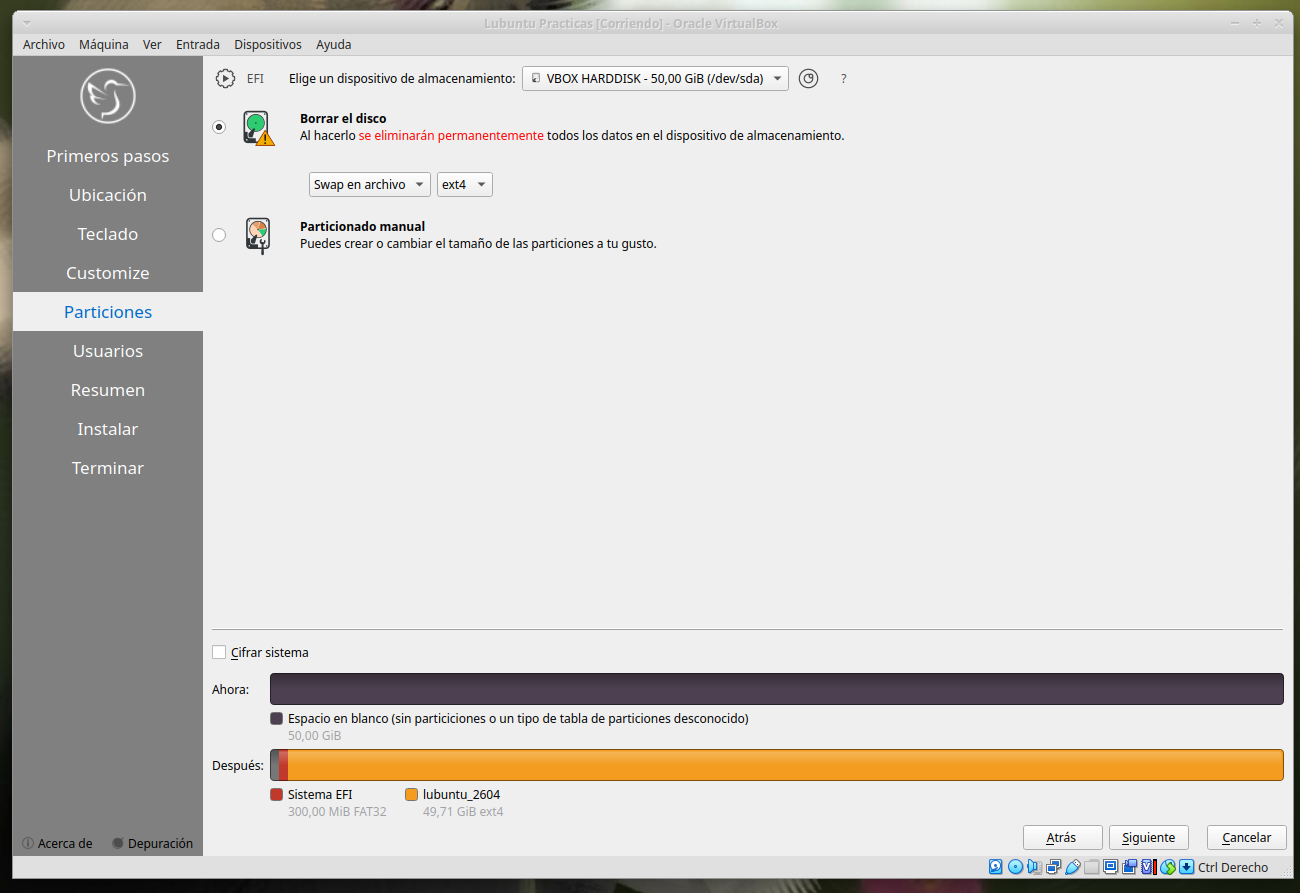
\includegraphics[width=0.8\textwidth]{15.png}
    \caption{Imagen 1}
    \label{fig:imagen1}
\end{figure}
\begin{figure}[ht]
    \centering
    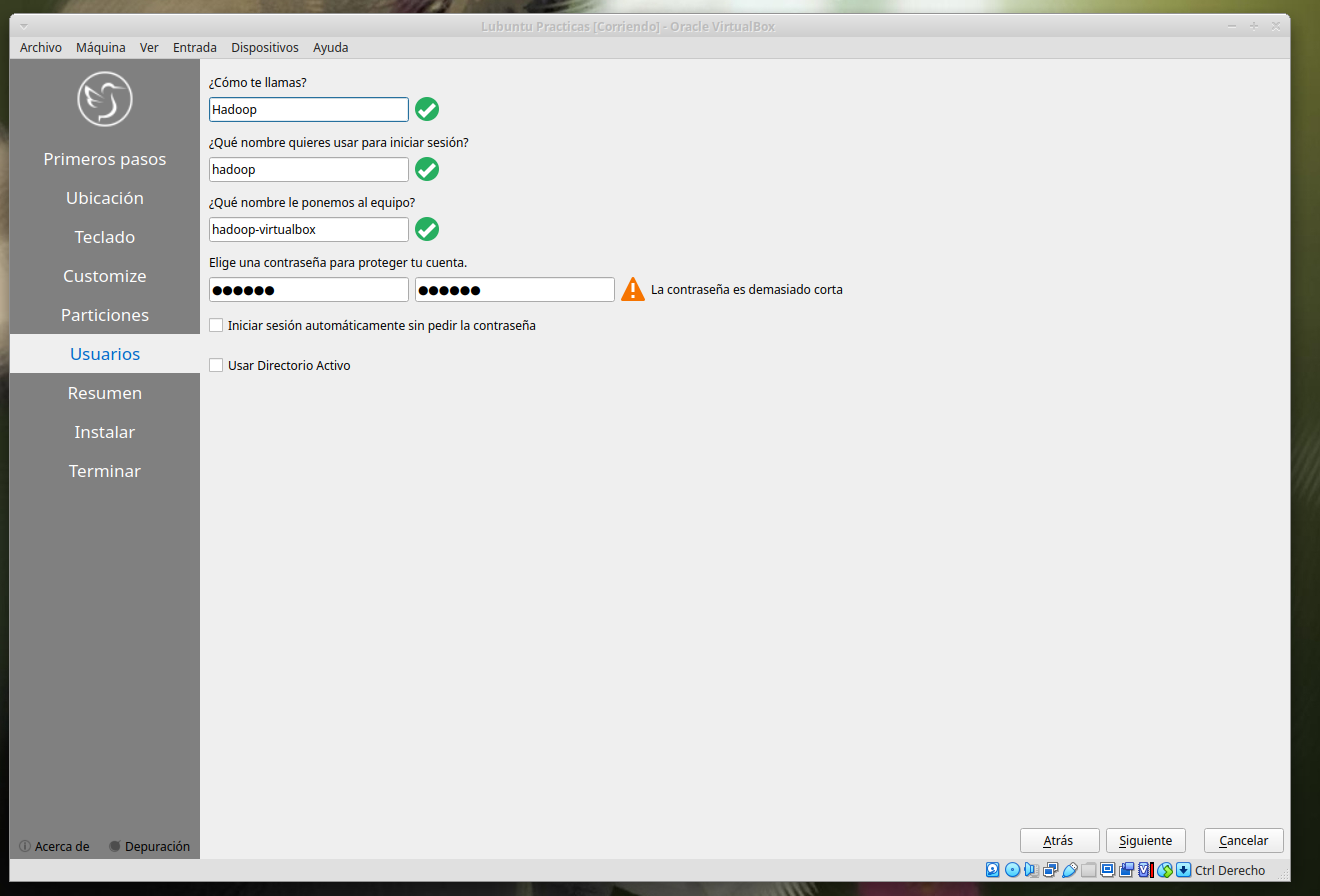
\includegraphics[width=0.8\textwidth]{16.png}
    \caption{Imagen 1}
    \label{fig:imagen1}
\end{figure}
\begin{figure}[ht]
    \centering
    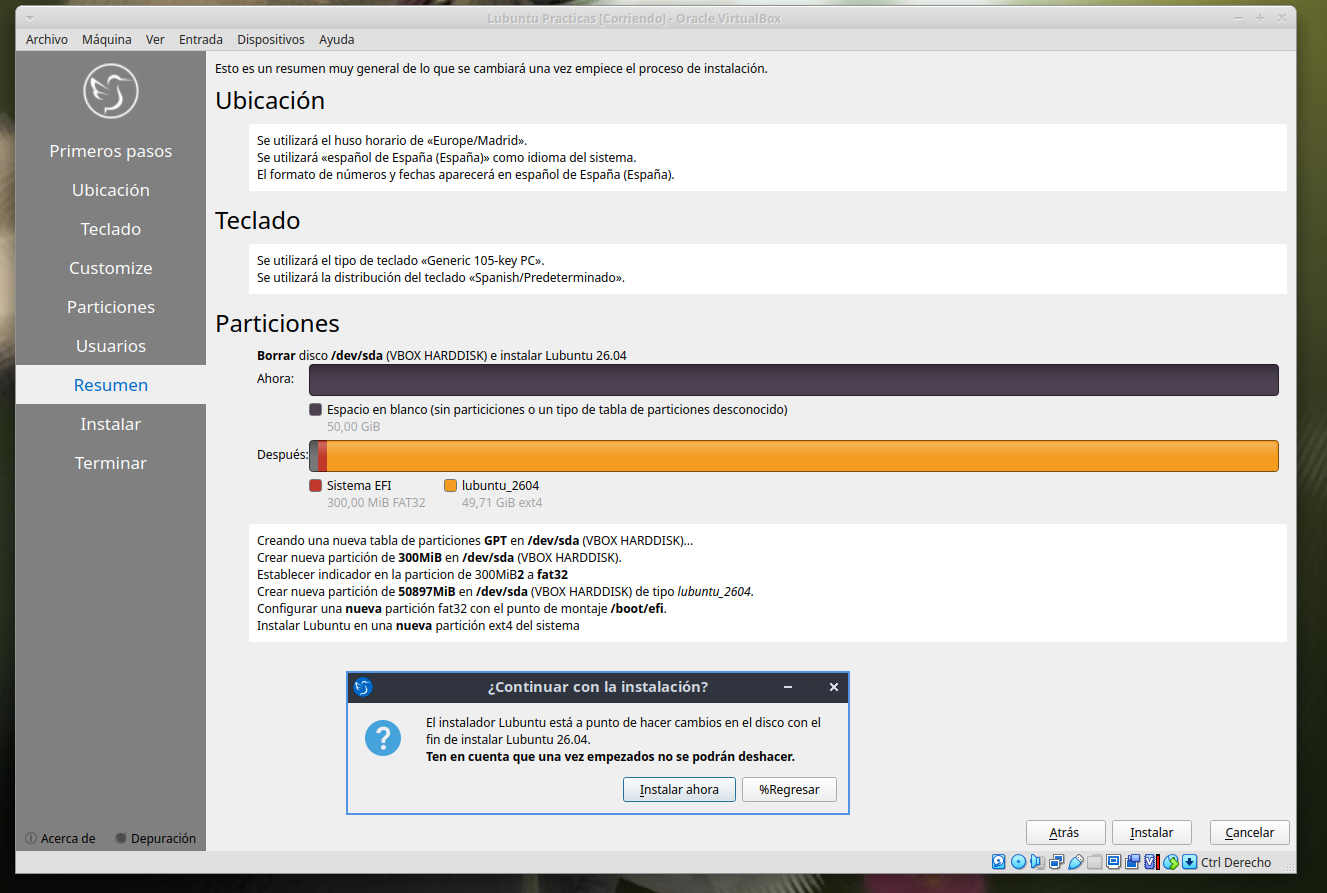
\includegraphics[width=0.8\textwidth]{17.png}
    \caption{Imagen 1}
    \label{fig:imagen1}
\end{figure}
\begin{figure}[ht]
    \centering
    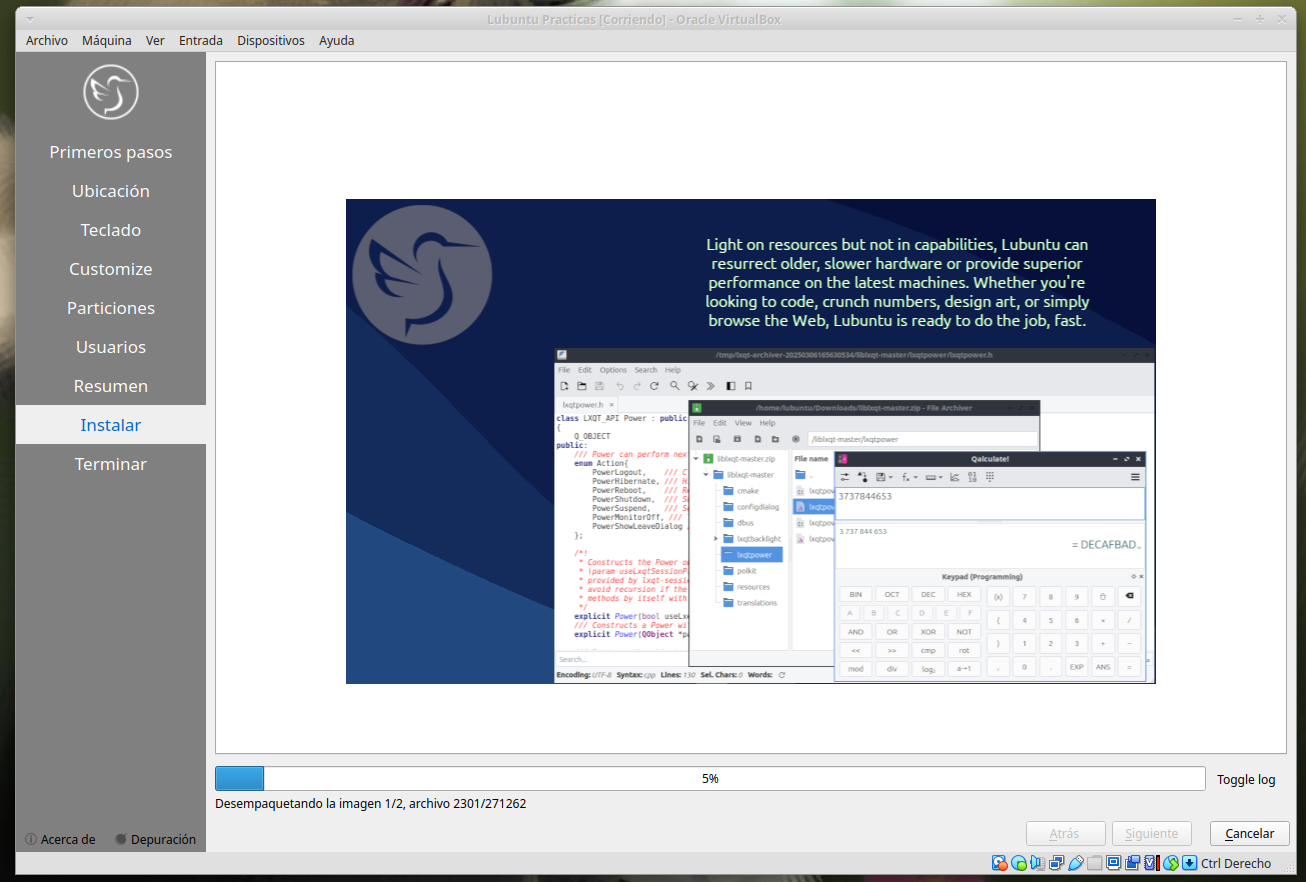
\includegraphics[width=0.8\textwidth]{18.png}
    \caption{Imagen 1}
    \label{fig:imagen1}
\end{figure}
\begin{figure}[ht]
    \centering
    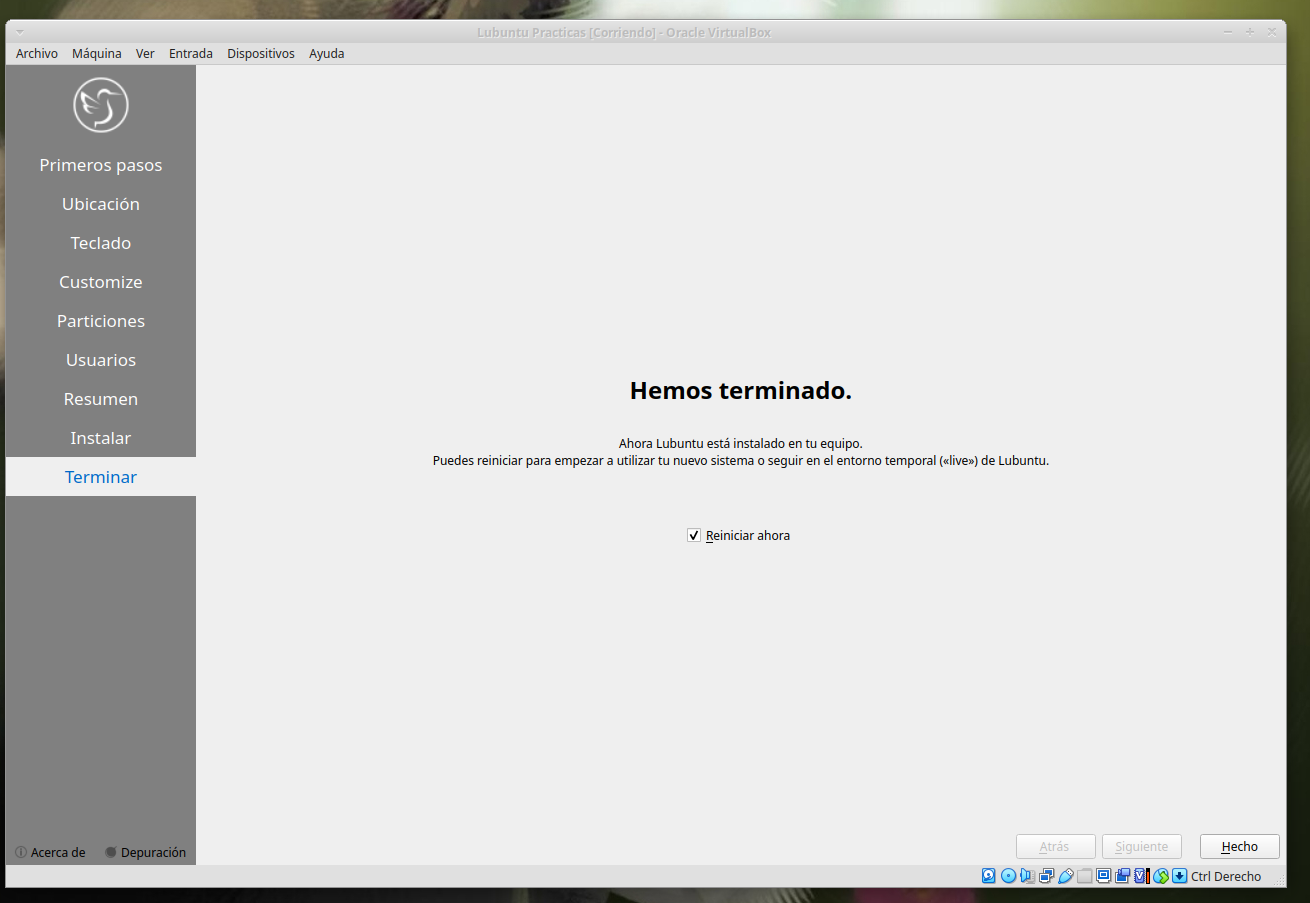
\includegraphics[width=0.8\textwidth]{19.png}
    \caption{Imagen 1}
    \label{fig:imagen1}
\end{figure}
\begin{figure}[ht]
    \centering
    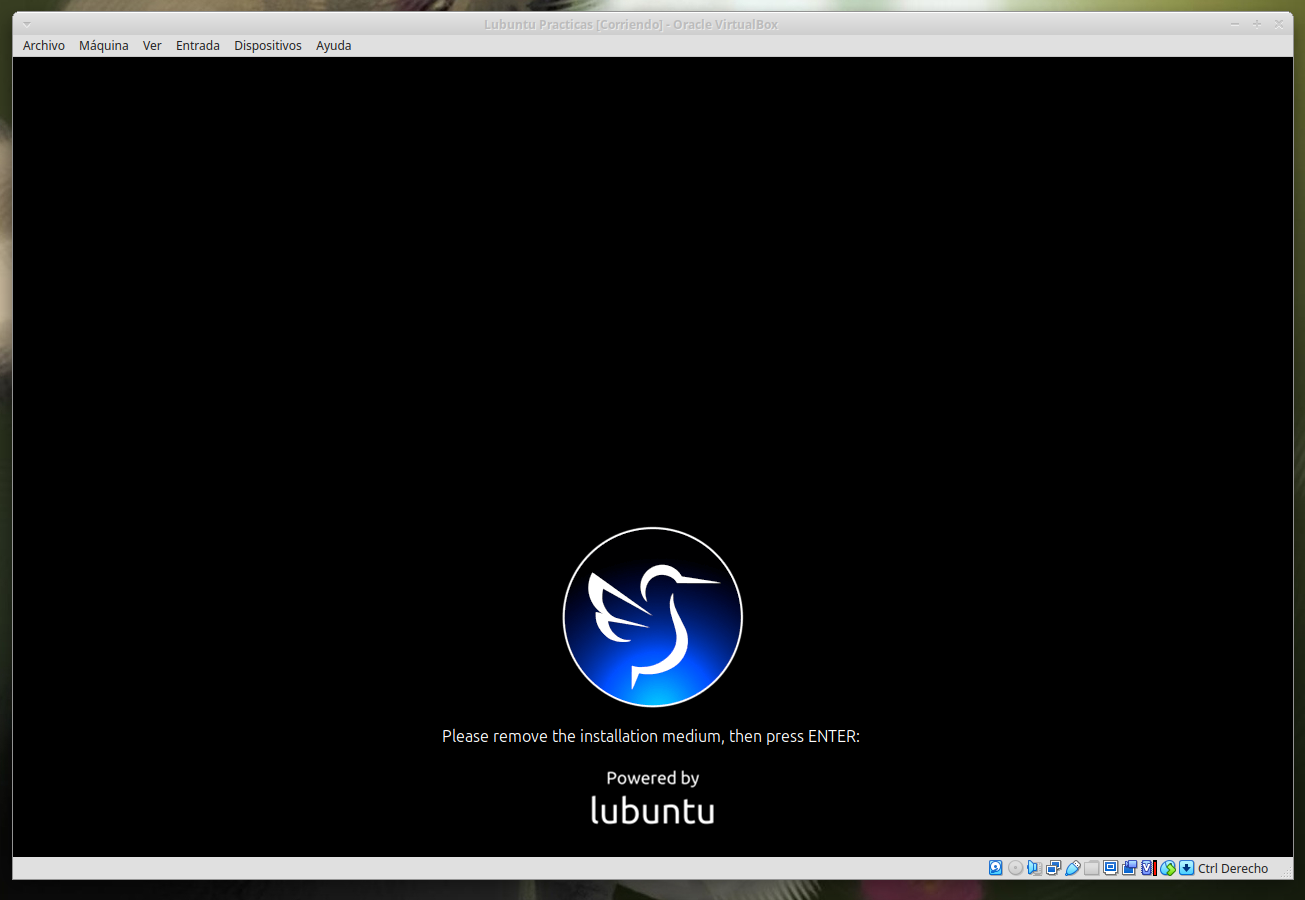
\includegraphics[width=0.8\textwidth]{20.png}
    \caption{Imagen 1}
    \label{fig:imagen1}
\end{figure}
\subsection{Preparación del sistema operativo}
\begin{figure}[ht]
    \centering
    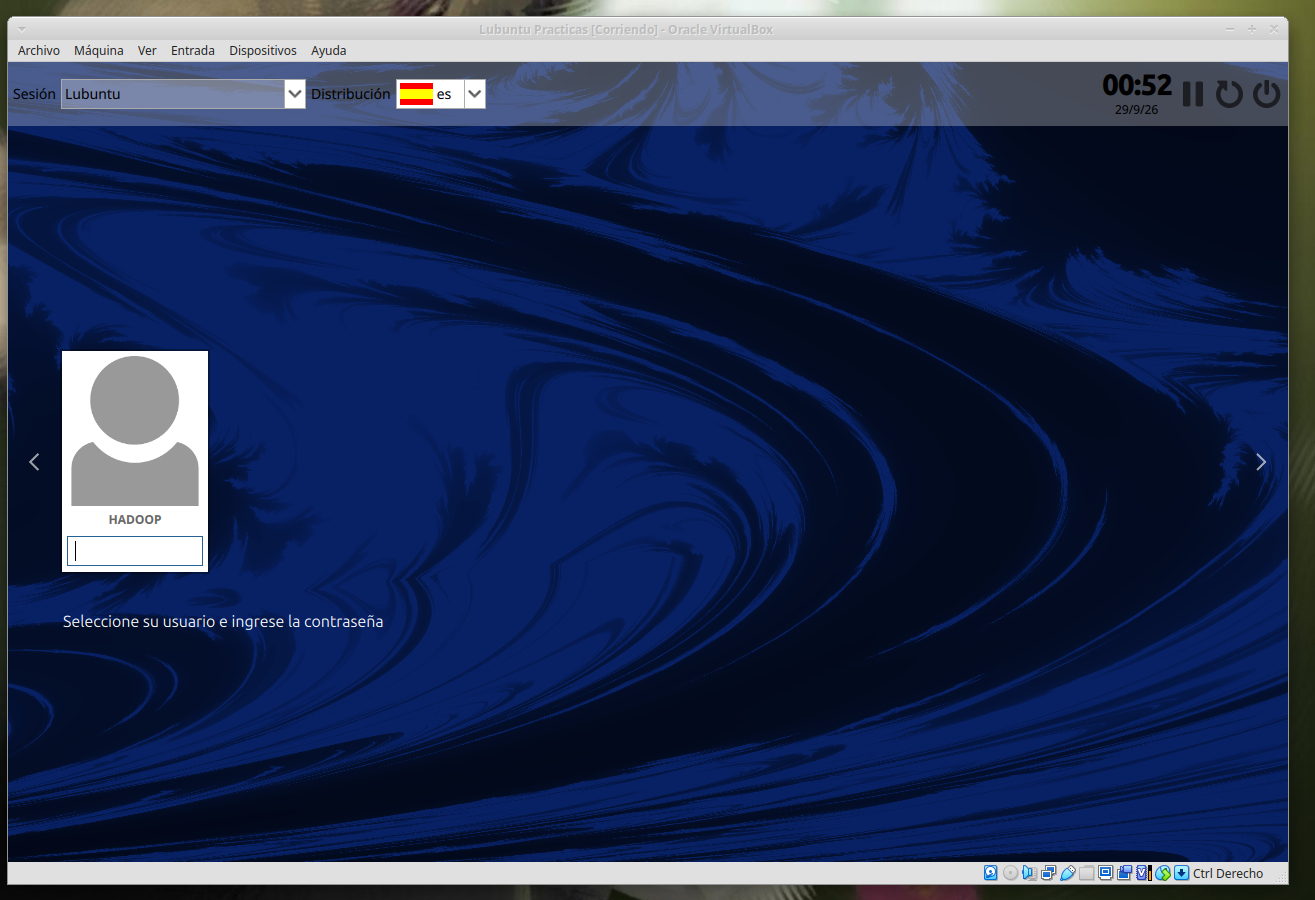
\includegraphics[width=0.8\textwidth]{21.png}
    \caption{Imagen 1}
    \label{fig:imagen1}
\end{figure}
\begin{figure}[ht]
    \centering
    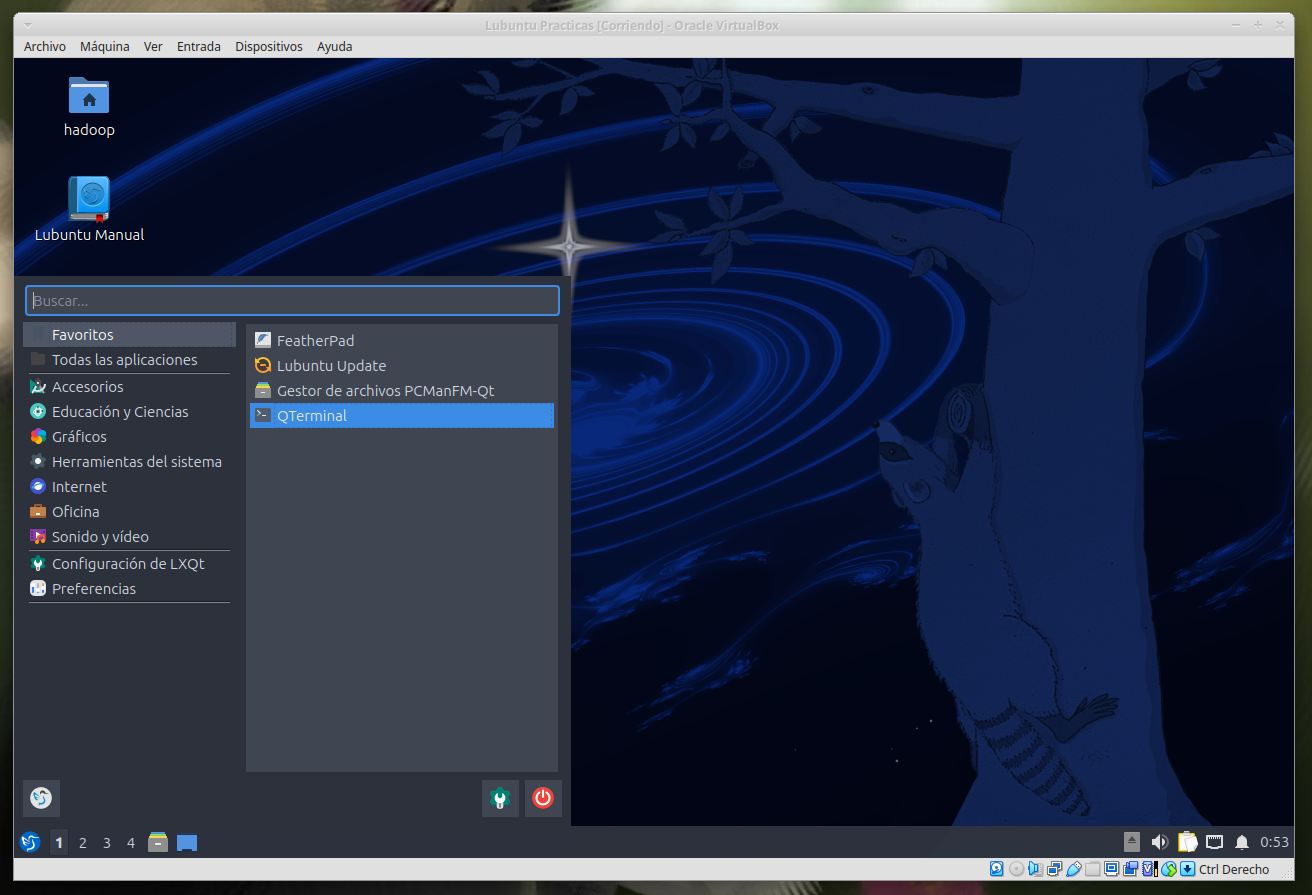
\includegraphics[width=0.8\textwidth]{22.png}
    \caption{Imagen 1}
    \label{fig:imagen1}
\end{figure}
\begin{figure}[ht]
    \centering
    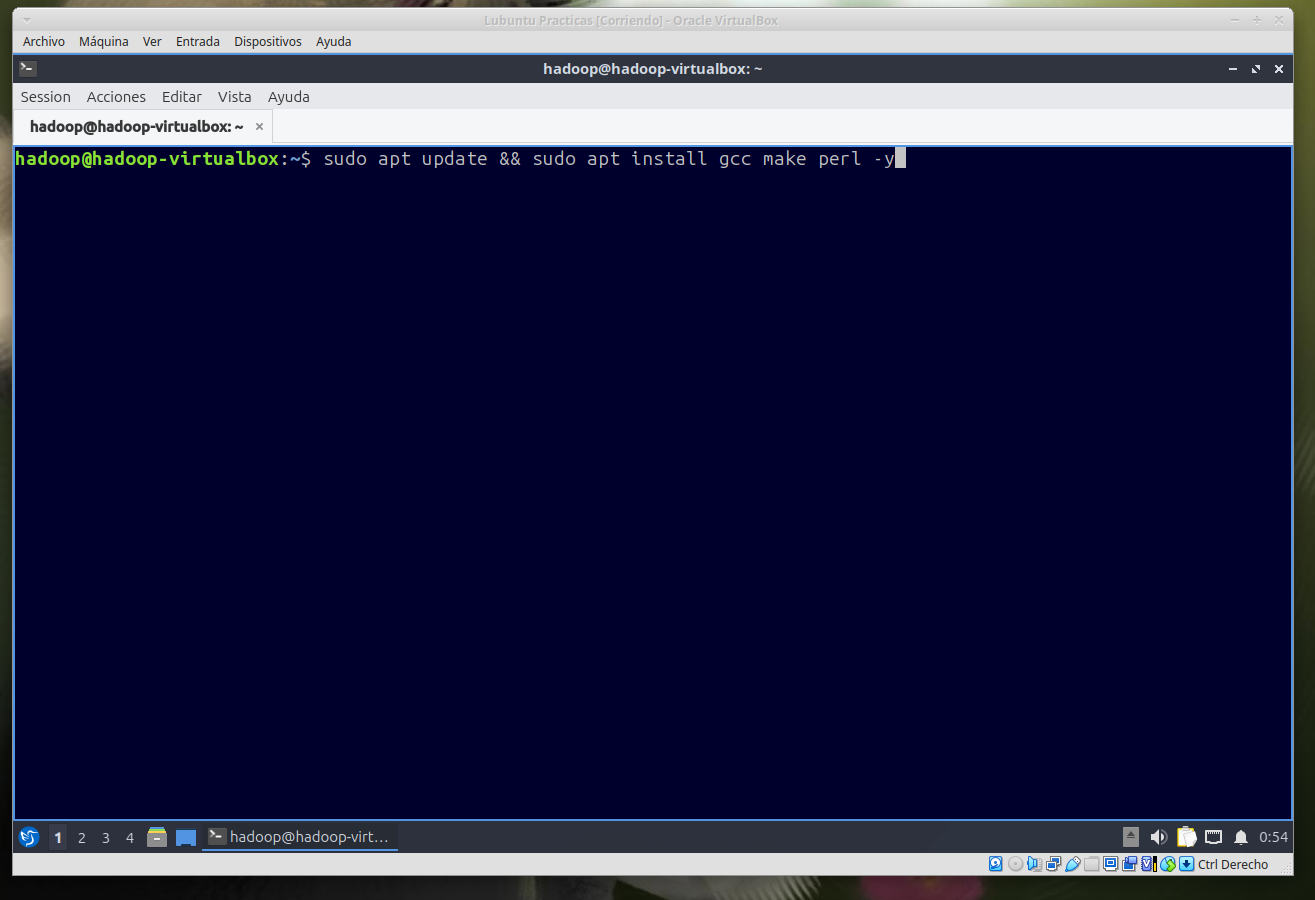
\includegraphics[width=0.8\textwidth]{23.png}
    \caption{Imagen 1}
    \label{fig:imagen1}
\end{figure}
\begin{figure}[ht]
    \centering
    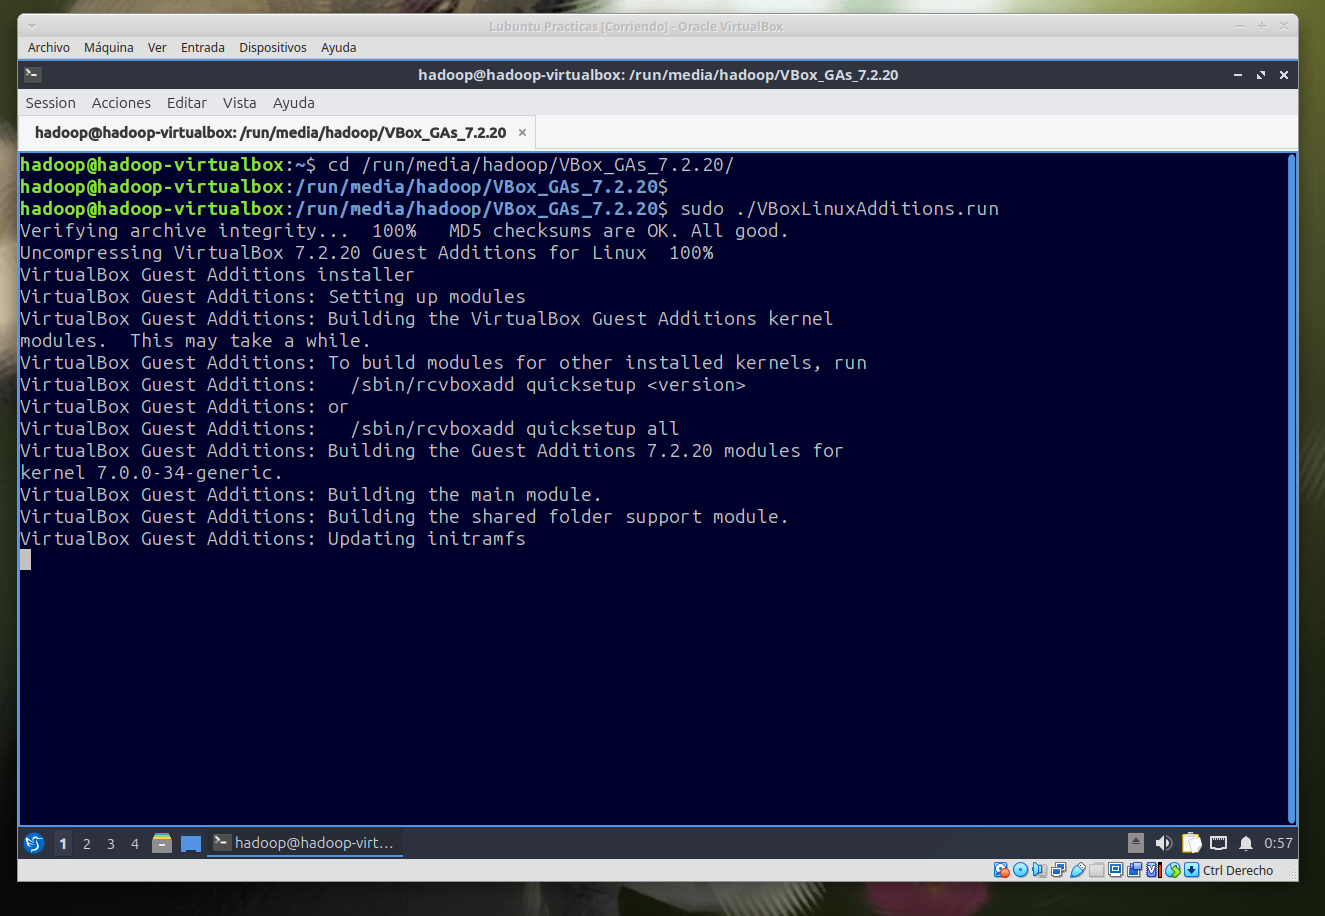
\includegraphics[width=0.8\textwidth]{24.png}
    \caption{Imagen 1}
    \label{fig:imagen1}
\end{figure}
\section{Practica 2 - Preparación del entorno, instalación y configuración de Apache NiFi}
\subsection{Instalación de JDK}
\begin{figure}[ht]
    \centering
    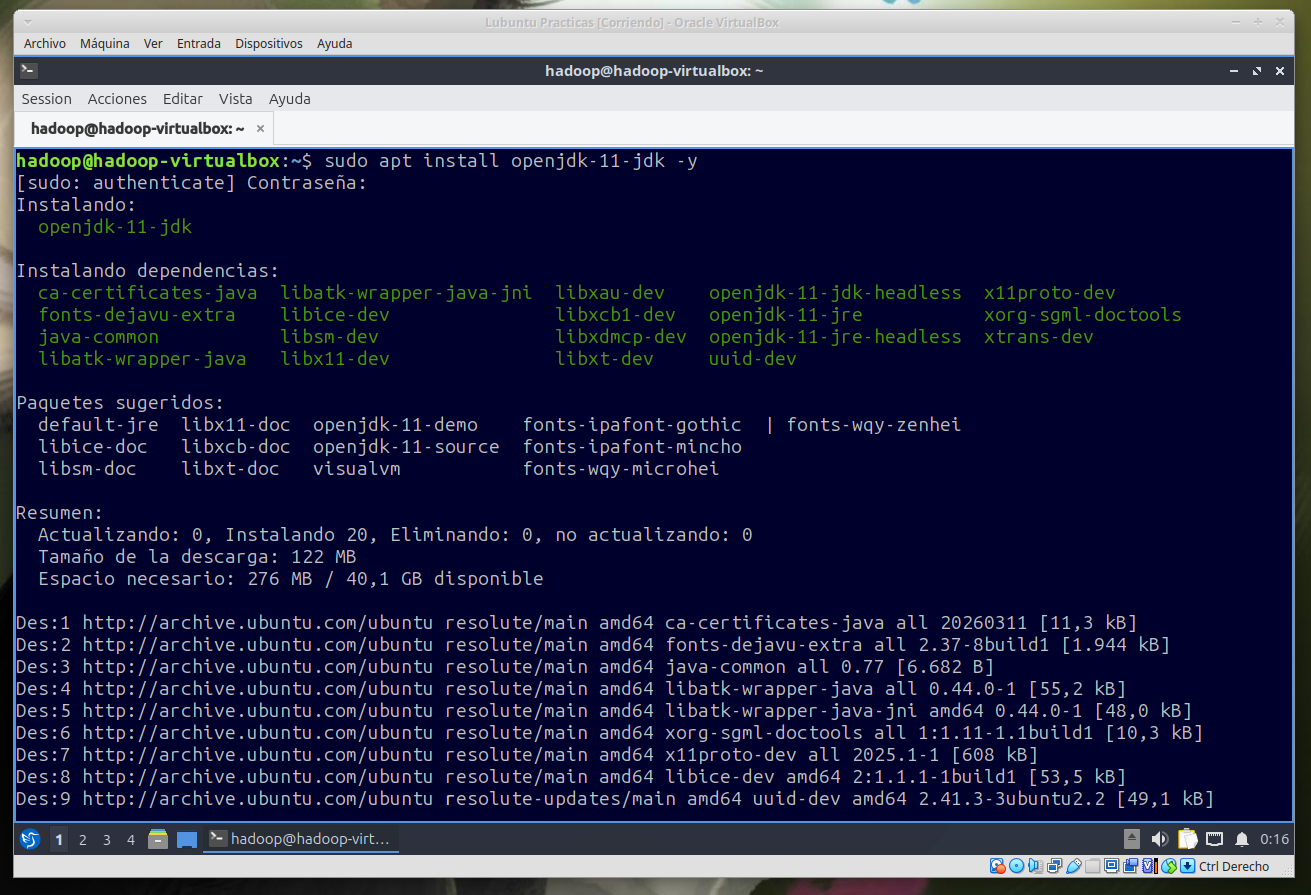
\includegraphics[width=0.8\textwidth]{25.png}
    \caption{Imagen 1}
    \label{fig:imagen1}
\end{figure}
\begin{figure}[ht]
    \centering
    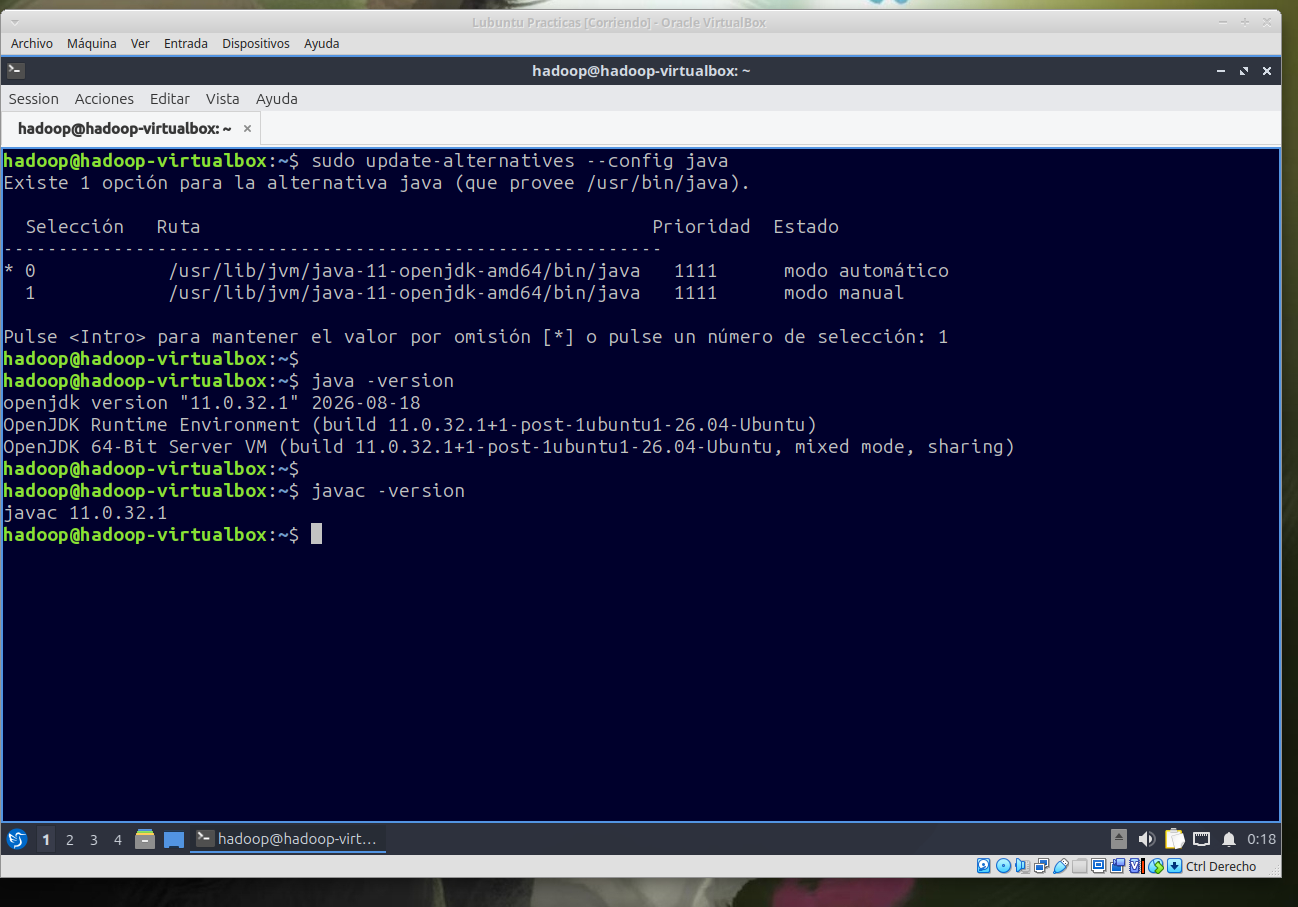
\includegraphics[width=0.8\textwidth]{26.png}
    \caption{Imagen 1}
    \label{fig:imagen1}
\end{figure}
\begin{figure}[ht]
    \centering
    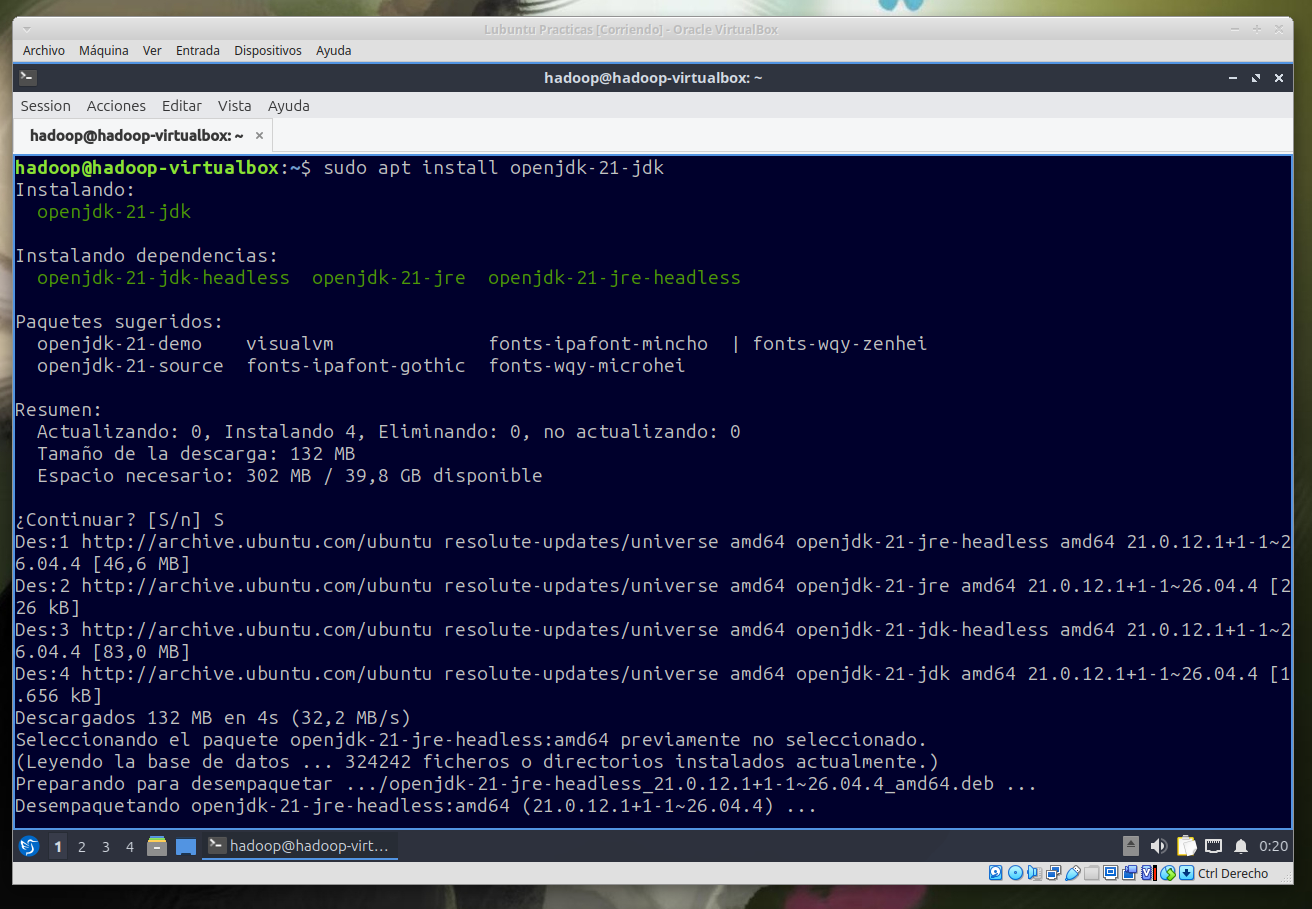
\includegraphics[width=0.8\textwidth]{27.png}
    \caption{Imagen 1}
    \label{fig:imagen1}
\end{figure}
\begin{figure}[ht]
    \centering
    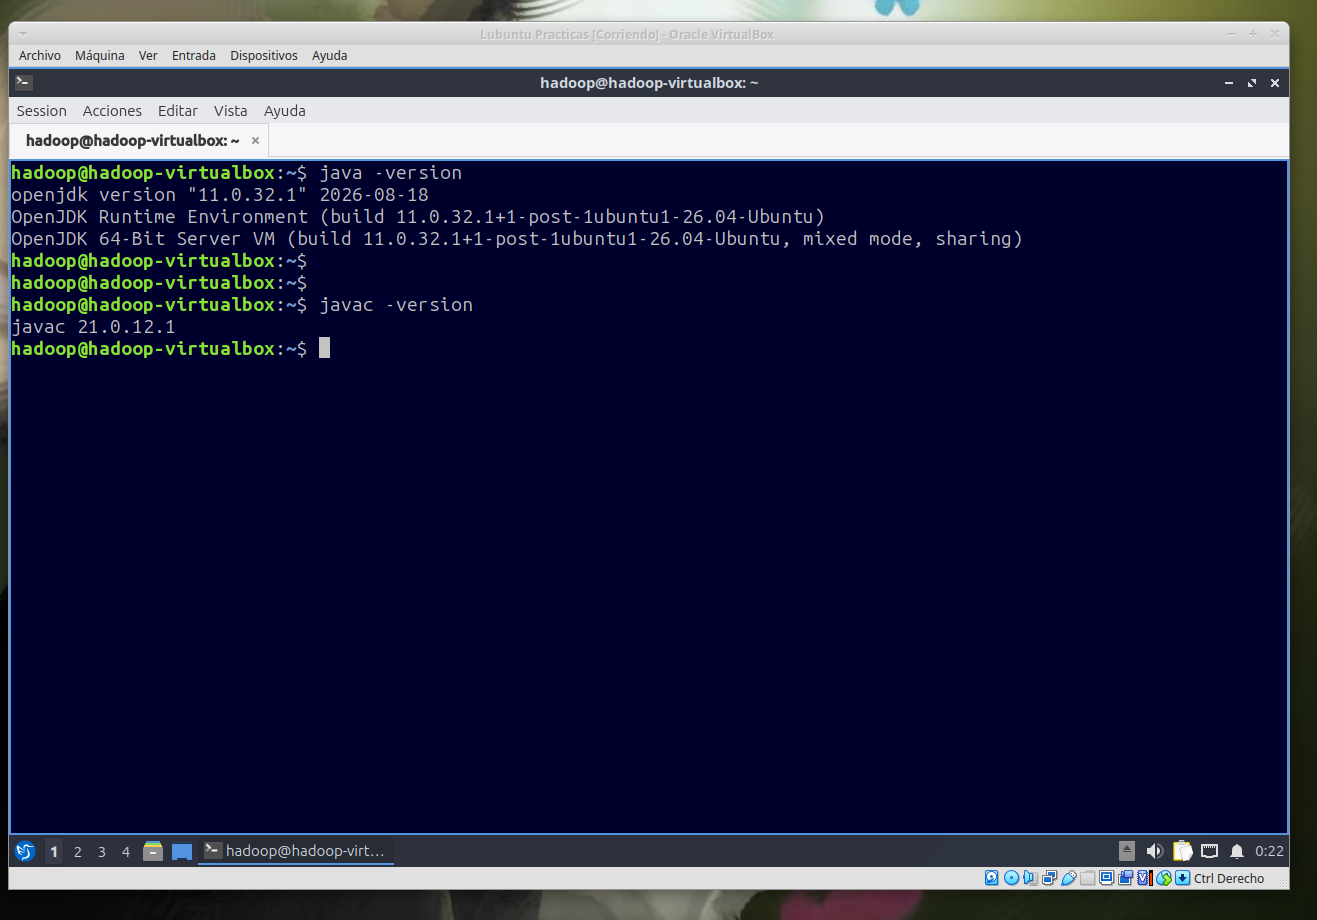
\includegraphics[width=0.8\textwidth]{28.png}
    \caption{Imagen 1}
    \label{fig:imagen1}
\end{figure}
\subsection{Creación de las variables de entorno de JAVA}
\begin{figure}[ht]
    \centering
    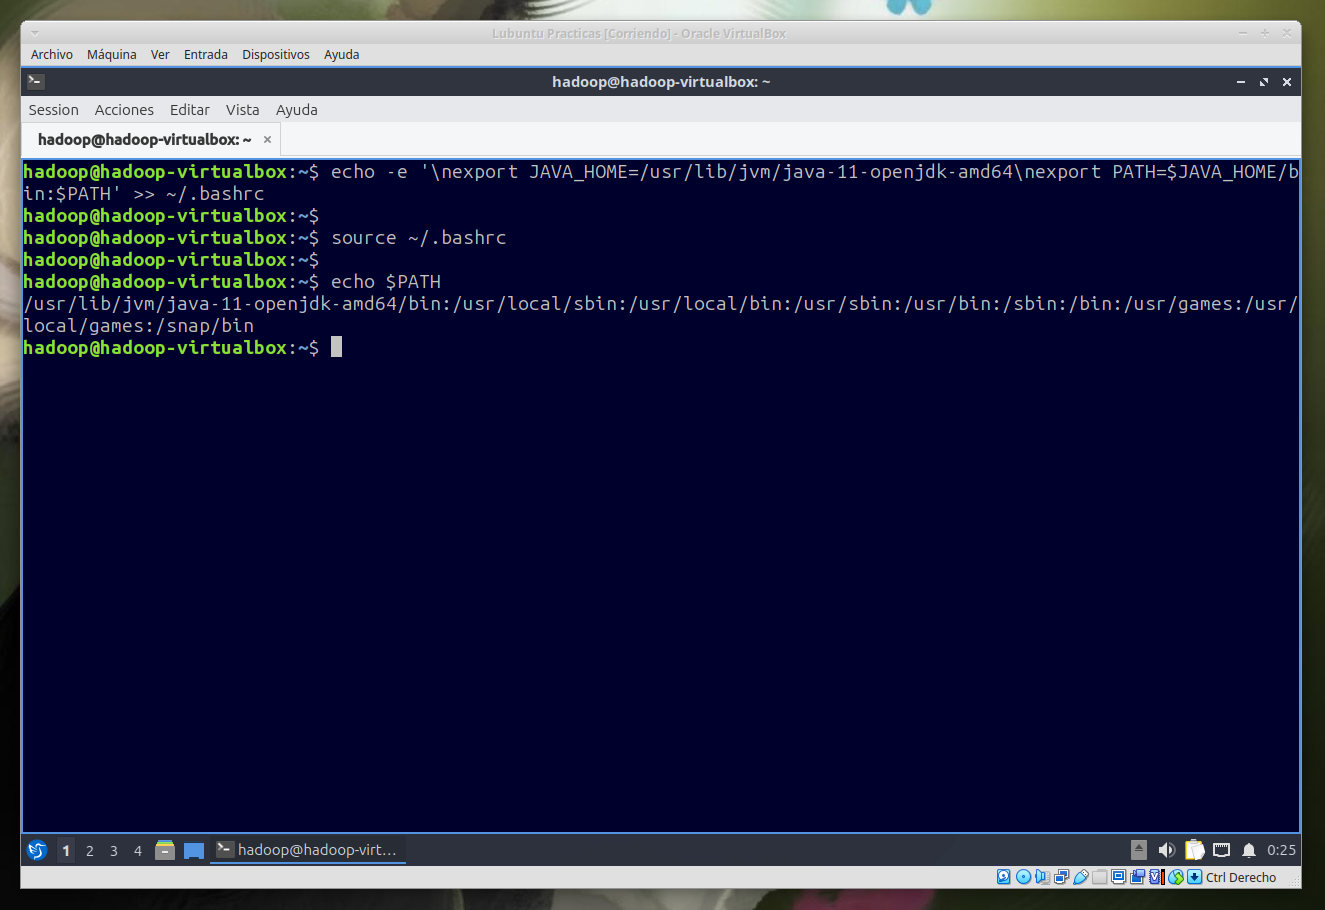
\includegraphics[width=0.8\textwidth]{29.png}
    \caption{Imagen 1}
    \label{fig:imagen1}
\end{figure}
\subsection{Instalacion de Nifi}
\begin{figure}[ht]
    \centering
    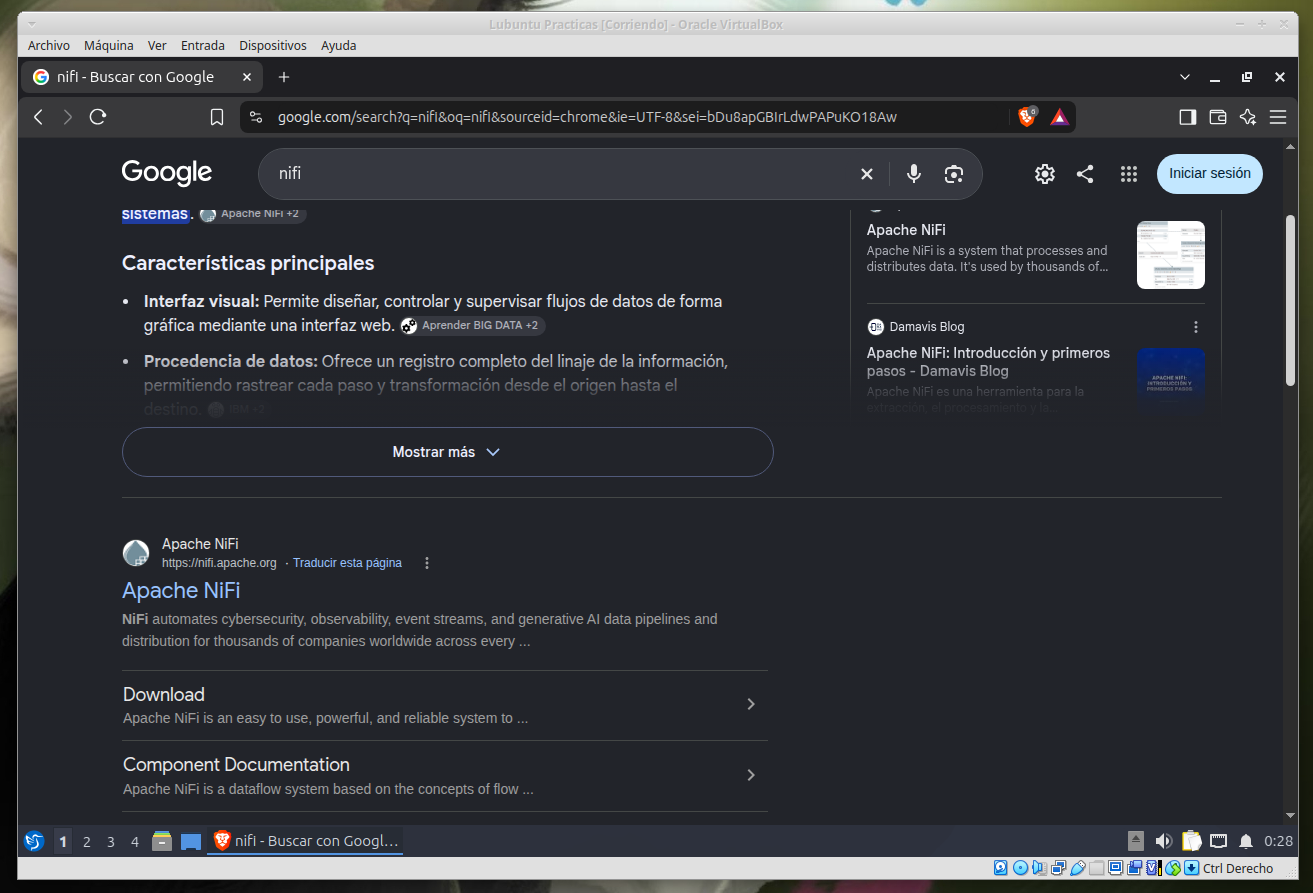
\includegraphics[width=0.8\textwidth]{30.png}
    \caption{Imagen 1}
    \label{fig:imagen1}
\end{figure}
\begin{figure}[ht]
    \centering
    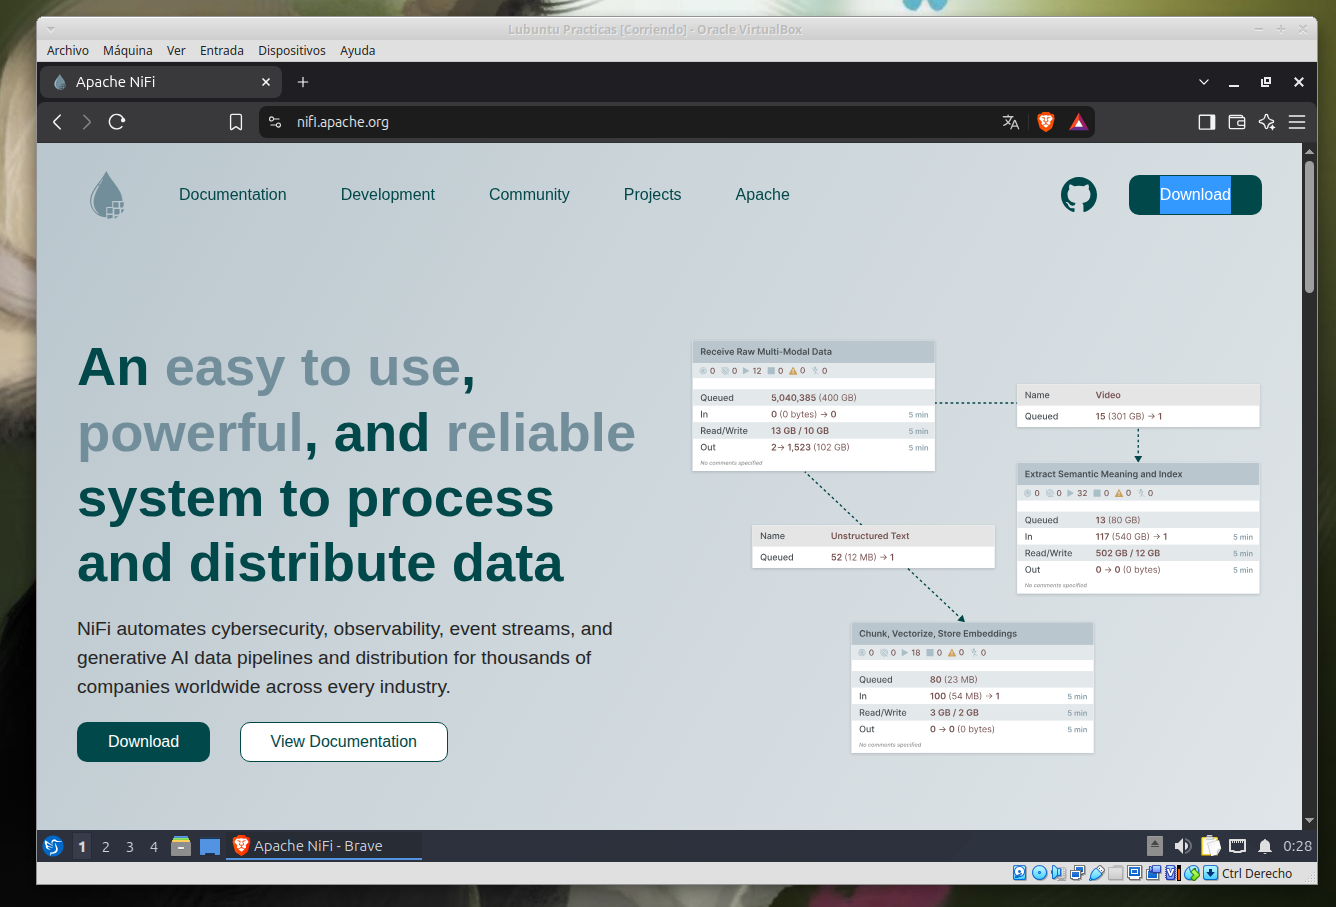
\includegraphics[width=0.8\textwidth]{31.png}
    \caption{Imagen 1}
    \label{fig:imagen1}
\end{figure}
\begin{figure}[ht]
    \centering
    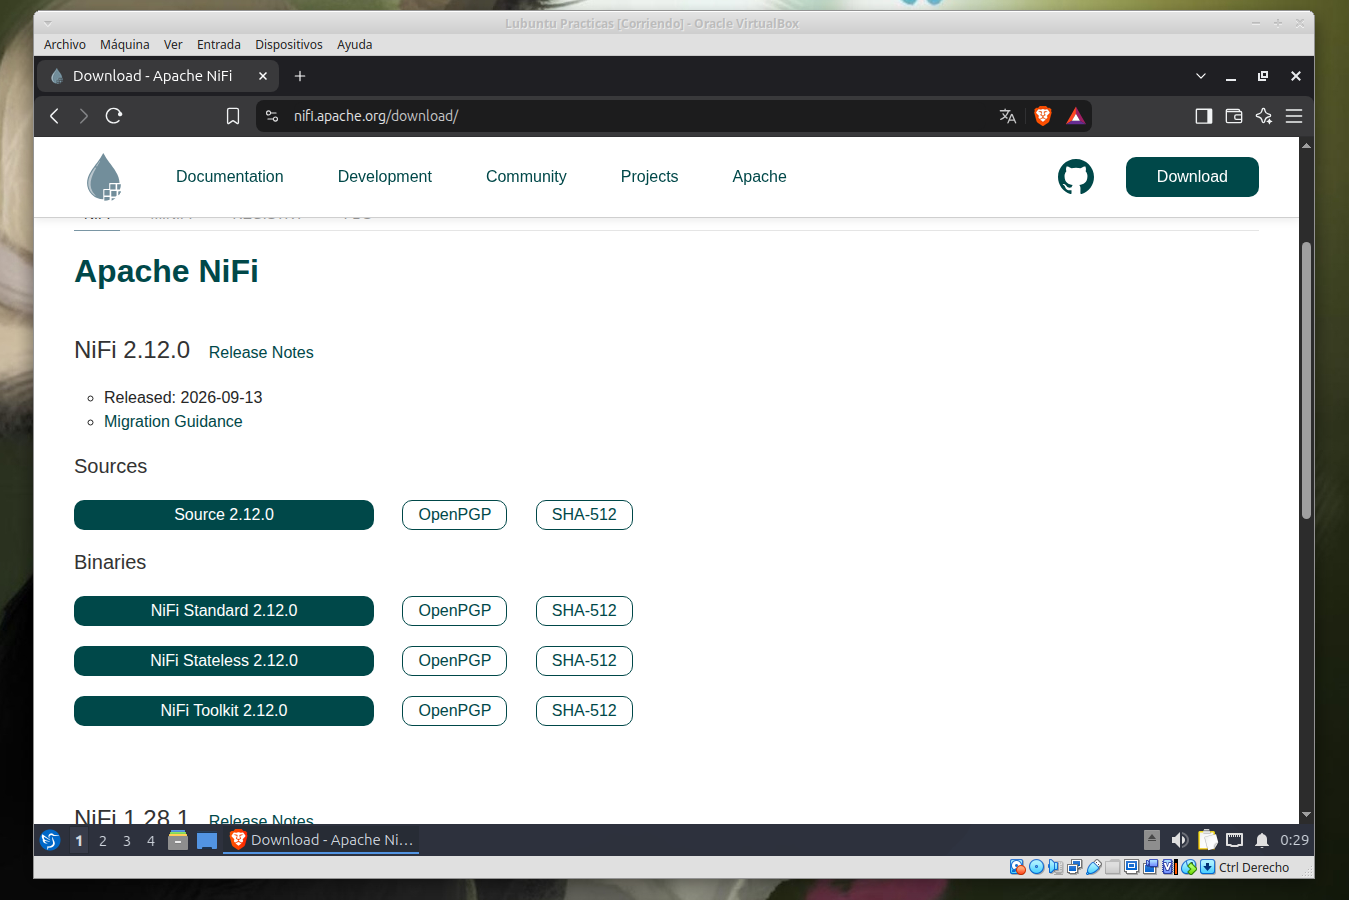
\includegraphics[width=0.8\textwidth]{32.png}
    \caption{Imagen 1}
    \label{fig:imagen1}
\end{figure}
\begin{figure}[ht]
    \centering
    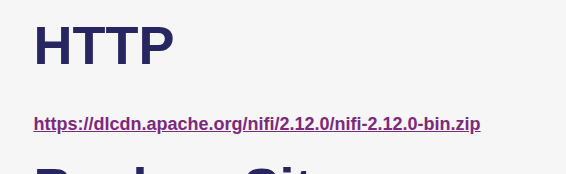
\includegraphics[width=0.8\textwidth]{33.png}
    \caption{Imagen 1}
    \label{fig:imagen1}
\end{figure}
\begin{figure}[ht]
    \centering
    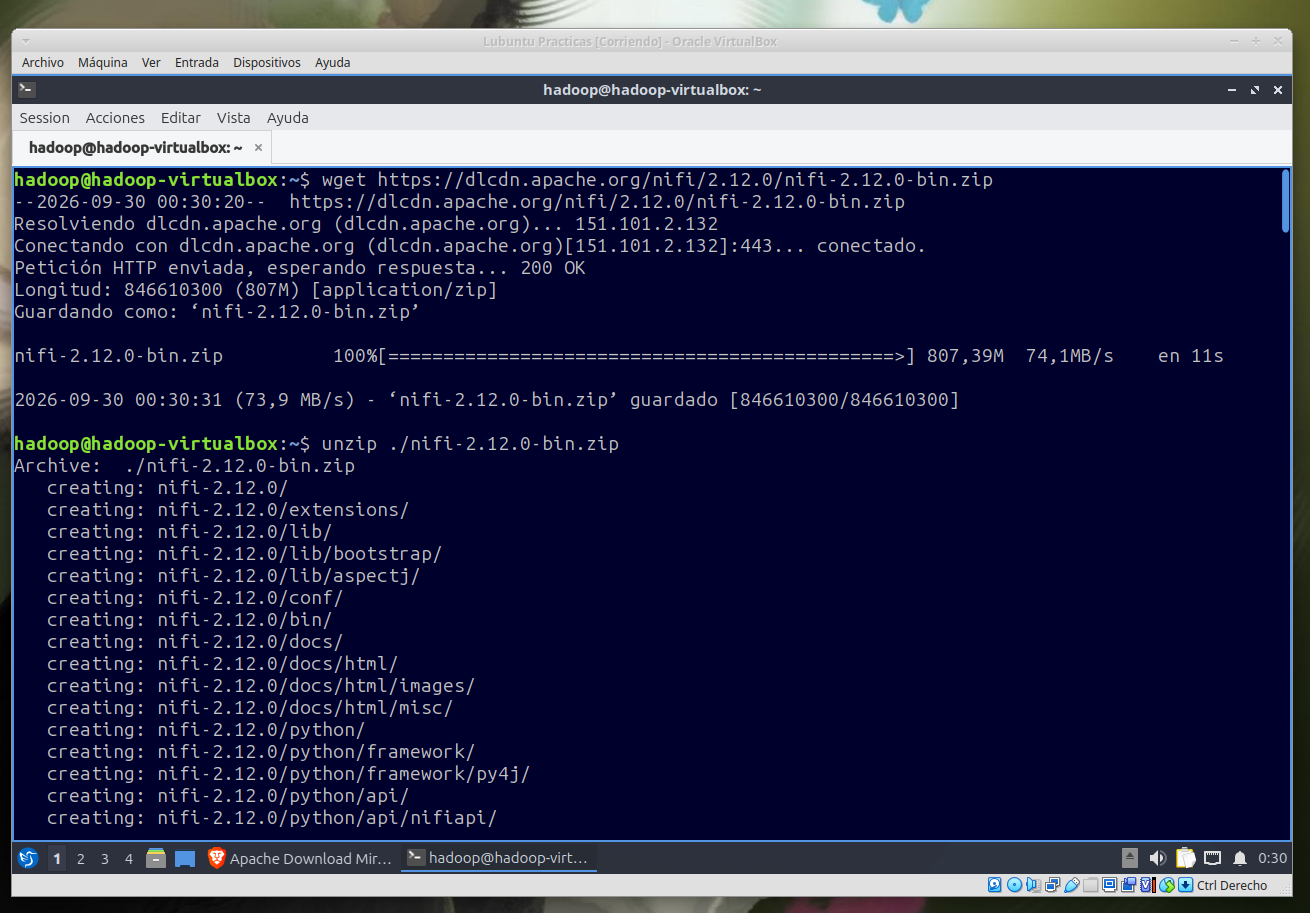
\includegraphics[width=0.8\textwidth]{34.png}
    \caption{Imagen 1}
    \label{fig:imagen1}
\end{figure}
\begin{figure}[ht]
    \centering
    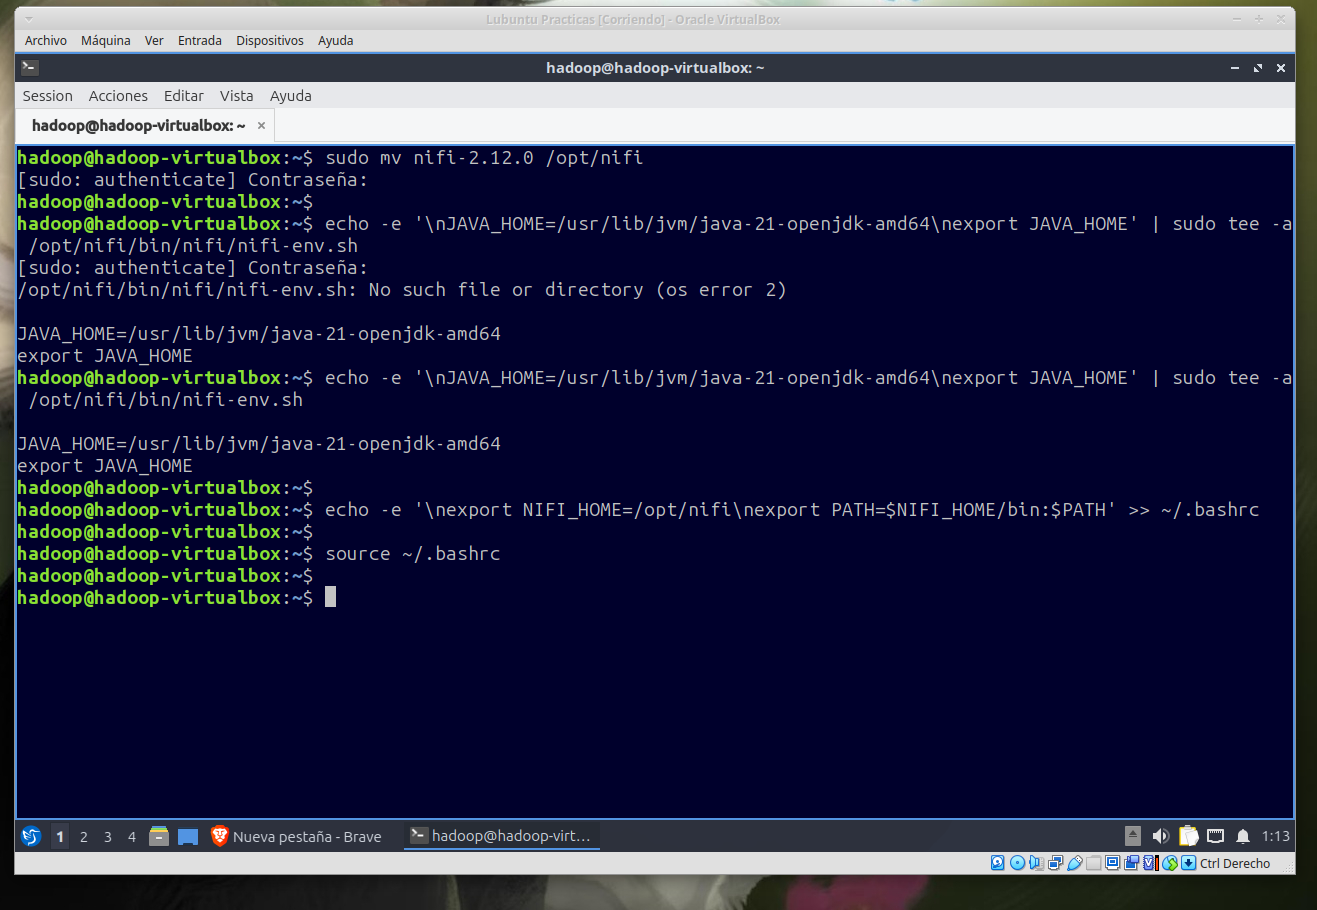
\includegraphics[width=0.8\textwidth]{35.png}
    \caption{Imagen 1}
    \label{fig:imagen1}
\end{figure}
\subsection{Creación de las variables de entorno de Nifi}
\begin{figure}[ht]
    \centering
    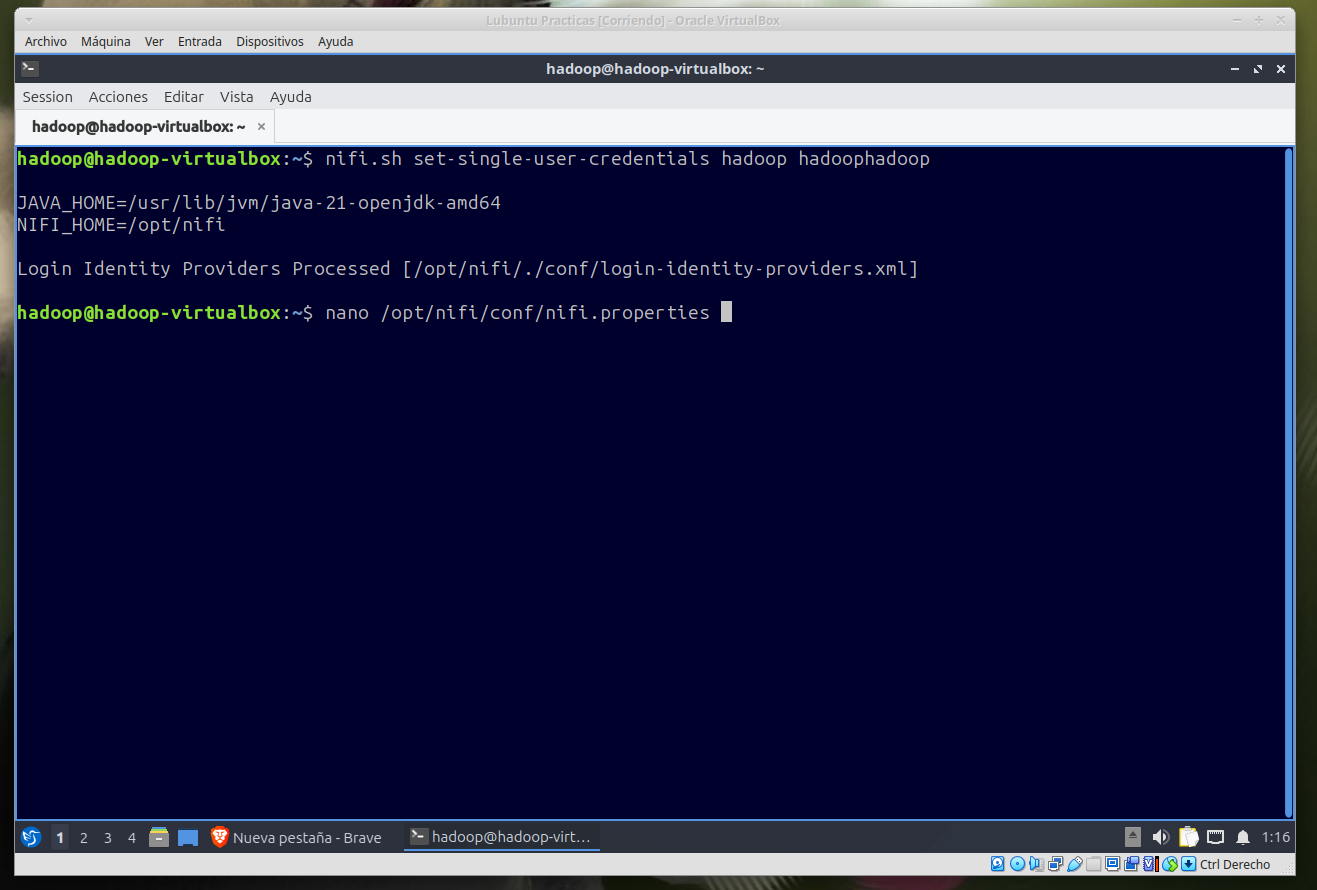
\includegraphics[width=0.8\textwidth]{36.png}
    \caption{Imagen 1}
    \label{fig:imagen1}
\end{figure}
\begin{figure}[ht]
    \centering
    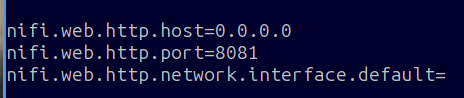
\includegraphics[width=0.8\textwidth]{37.png}
    \caption{Imagen 1}
    \label{fig:imagen1}
\end{figure}
\begin{figure}[ht]
    \centering
    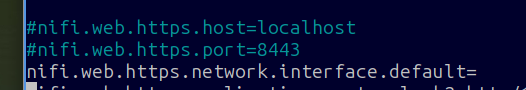
\includegraphics[width=0.8\textwidth]{38.png}
    \caption{Imagen 1}
    \label{fig:imagen1}
\end{figure}
\begin{figure}[ht]
    \centering
    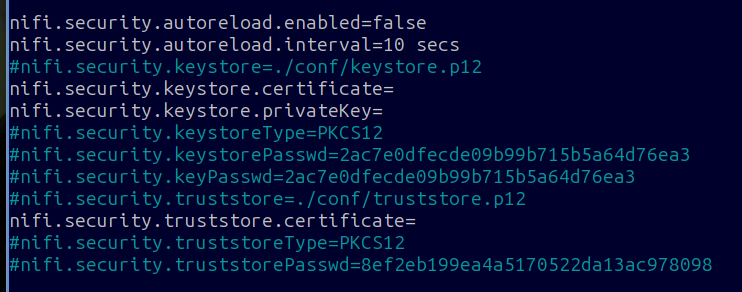
\includegraphics[width=0.8\textwidth]{39.png}
    \caption{Imagen 1}
    \label{fig:imagen1}
\end{figure}
\begin{figure}[ht]
    \centering
    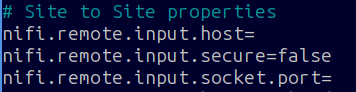
\includegraphics[width=0.8\textwidth]{40.png}
    \caption{Imagen 1}
    \label{fig:imagen1}
\end{figure}
\subsection{Arranque de Nifi y configuración}
\begin{figure}[ht]
    \centering
    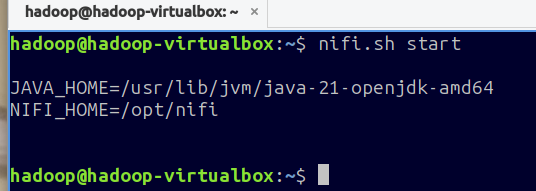
\includegraphics[width=0.8\textwidth]{41.png}
    \caption{Imagen 1}
    \label{fig:imagen1}
\end{figure}
\begin{figure}[ht]
    \centering
    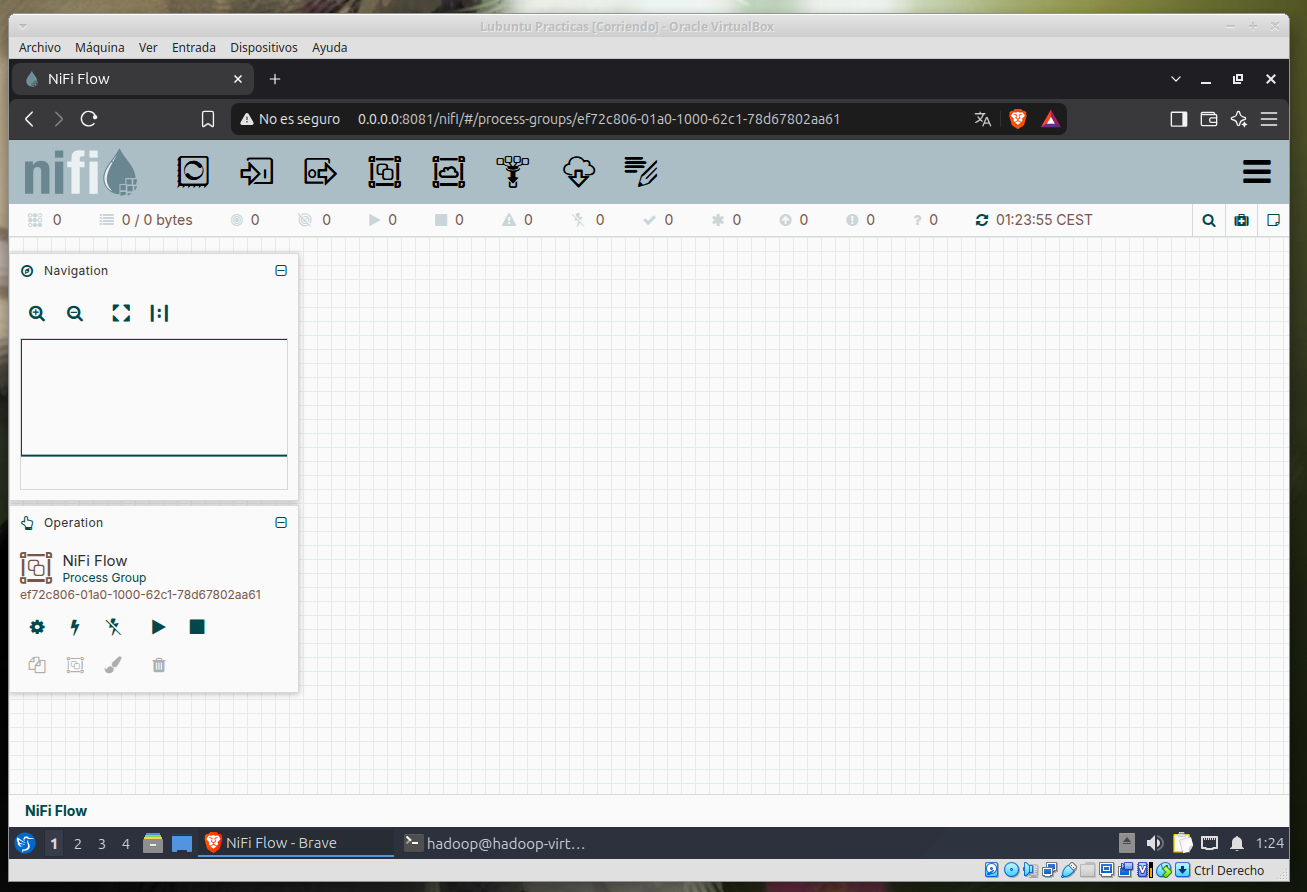
\includegraphics[width=0.8\textwidth]{42.png}
    \caption{Imagen 1}
    \label{fig:imagen1}
\end{figure}
\section{Practica 3 - Practicando el manejo de ficheros}
\subsection{Preparación de directorios y procesos}
\begin{figure}[ht]
    \centering
    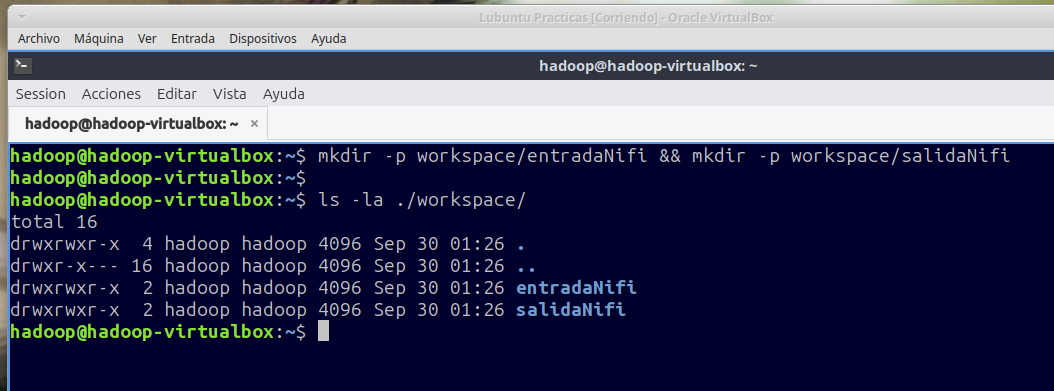
\includegraphics[width=0.8\textwidth]{43.png}
    \caption{Imagen 1}
    \label{fig:imagen1}
\end{figure}
\begin{figure}[ht]
    \centering
    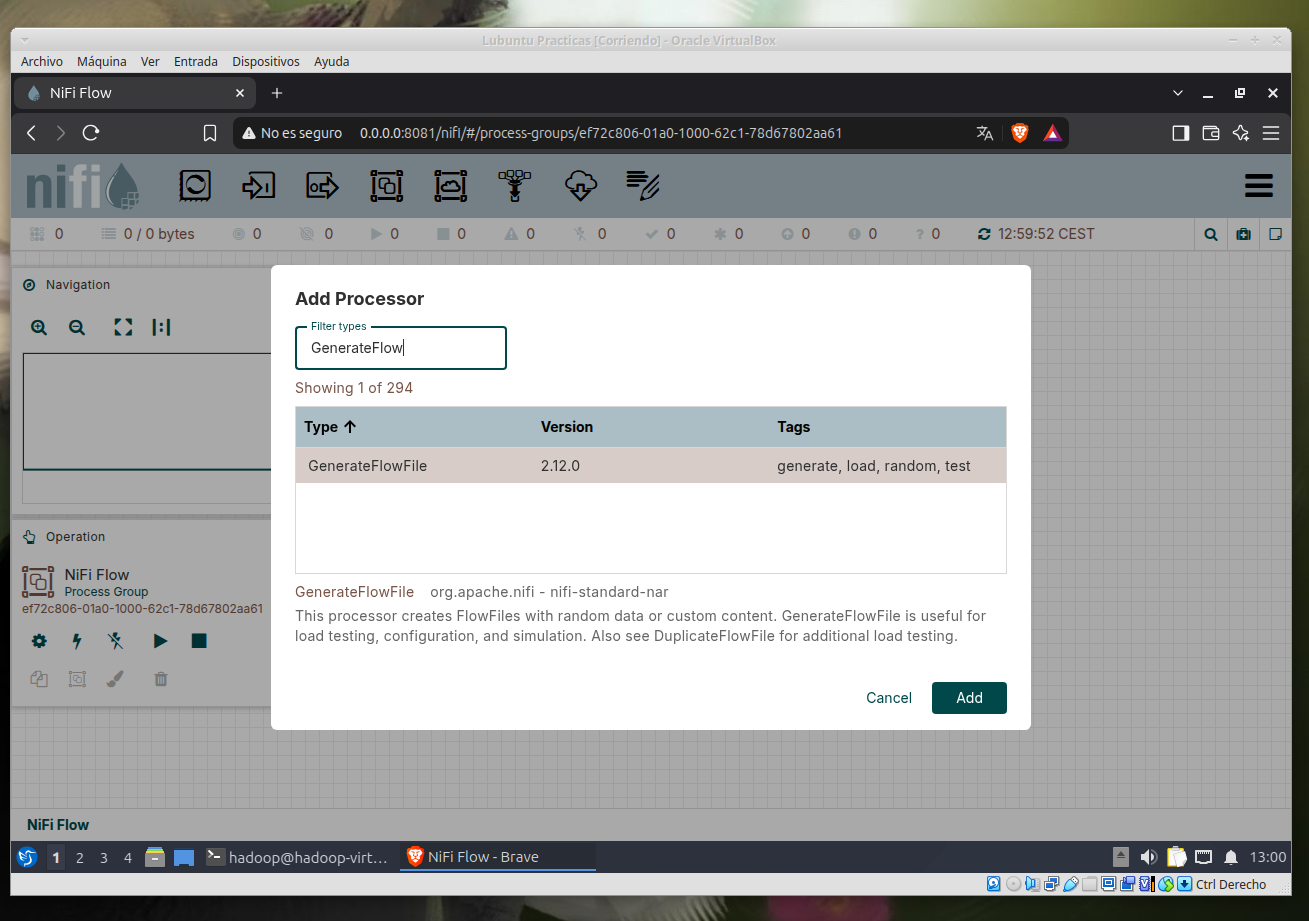
\includegraphics[width=0.8\textwidth]{44.png}
    \caption{Imagen 1}
    \label{fig:imagen1}
\end{figure}
\begin{figure}[ht]
    \centering
    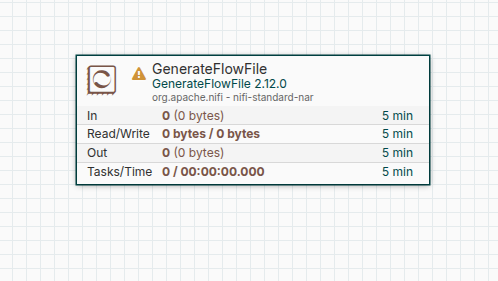
\includegraphics[width=0.8\textwidth]{45.png}
    \caption{Imagen 1}
    \label{fig:imagen1}
\end{figure}
\begin{figure}[ht]
    \centering
    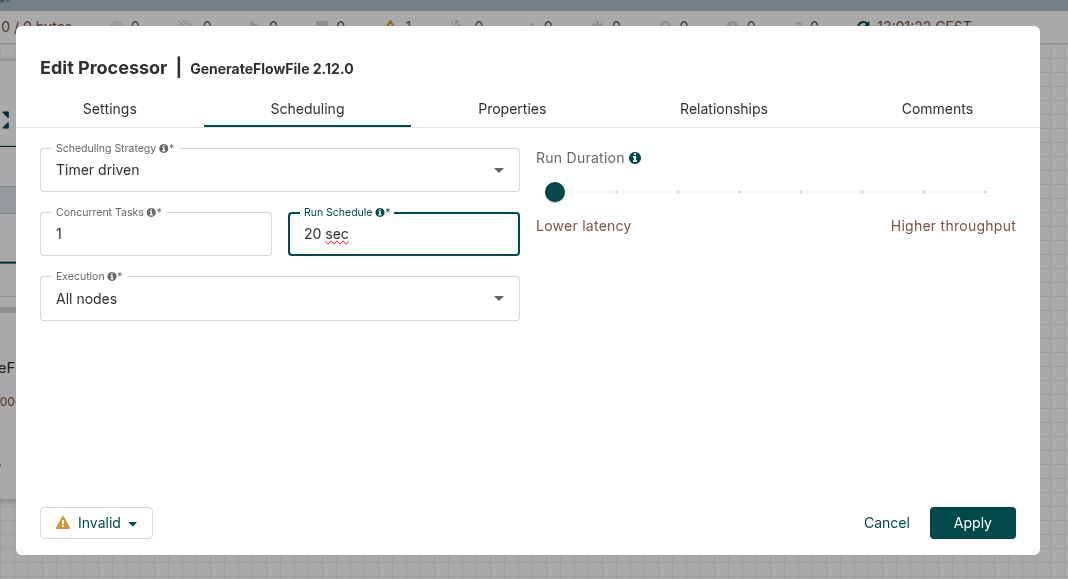
\includegraphics[width=0.8\textwidth]{46.png}
    \caption{Imagen 1}
    \label{fig:imagen1}
\end{figure}
\begin{figure}[ht]
    \centering
    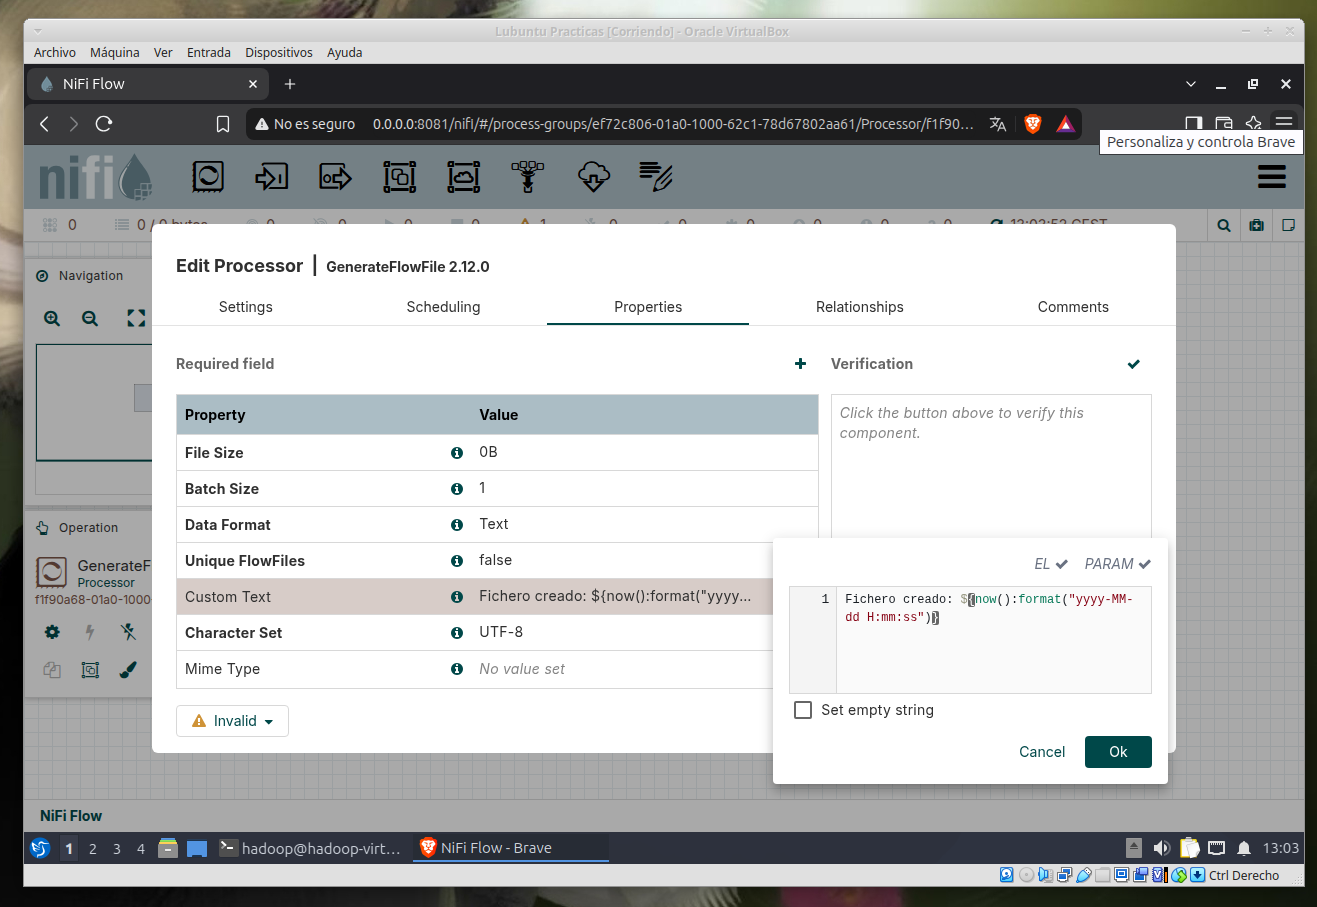
\includegraphics[width=0.8\textwidth]{47.png}
    \caption{Imagen 1}
    \label{fig:imagen1}
\end{figure}
\subsection{Definición de atributo}
\begin{figure}[ht]
    \centering
    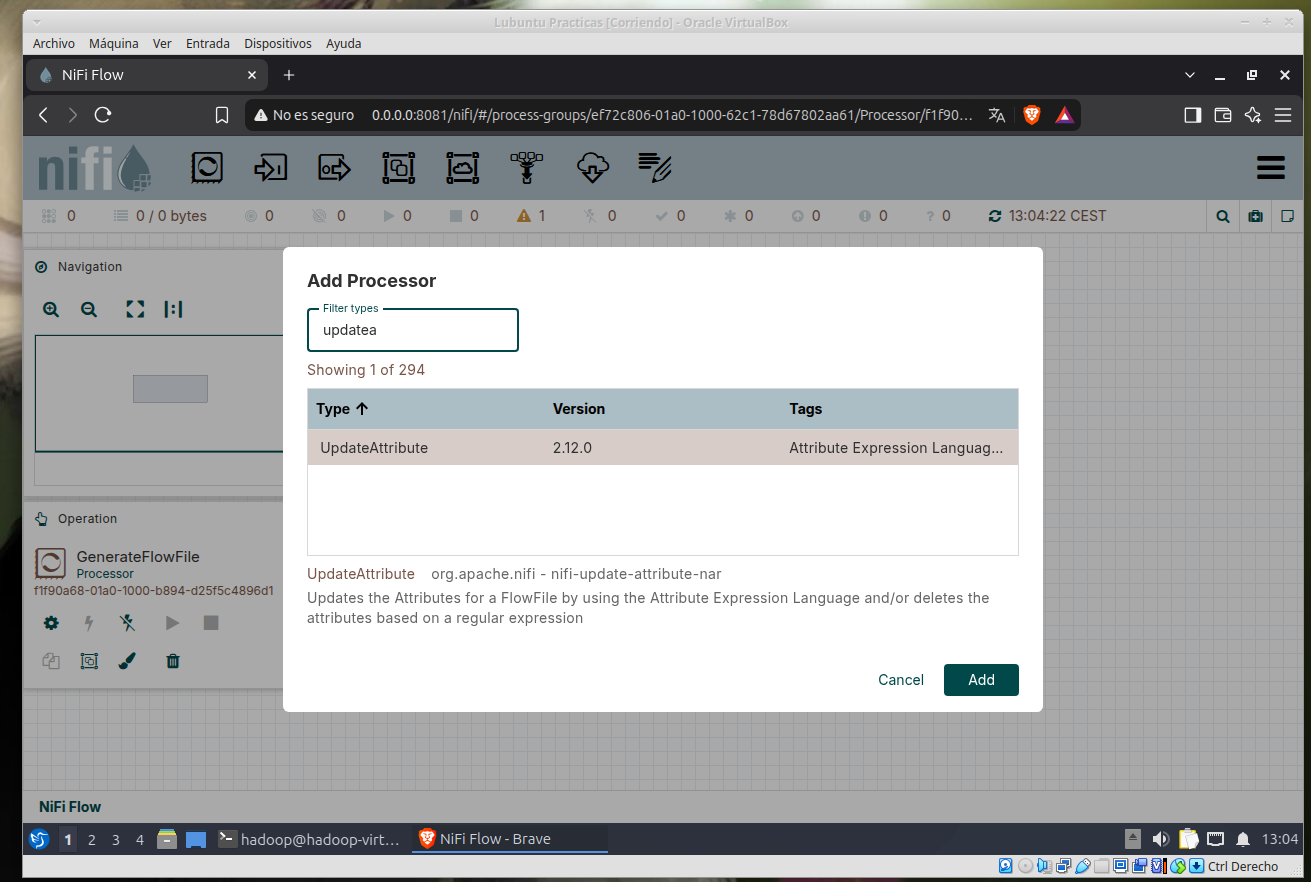
\includegraphics[width=0.8\textwidth]{48.png}
    \caption{Imagen 1}
    \label{fig:imagen1}
\end{figure}
\begin{figure}[ht]
    \centering
    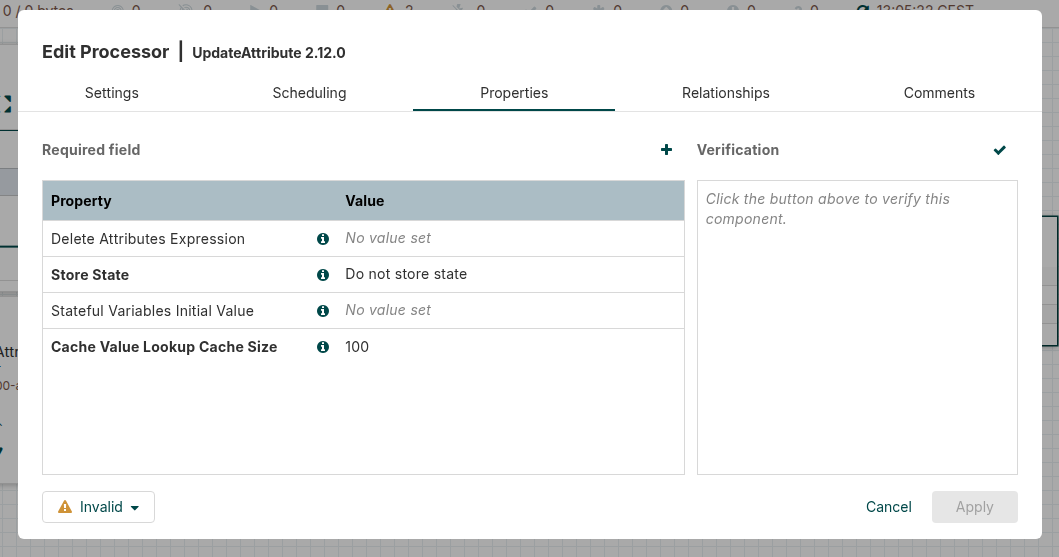
\includegraphics[width=0.8\textwidth]{49.png}
    \caption{Imagen 1}
    \label{fig:imagen1}
\end{figure}
\begin{figure}[ht]
    \centering
    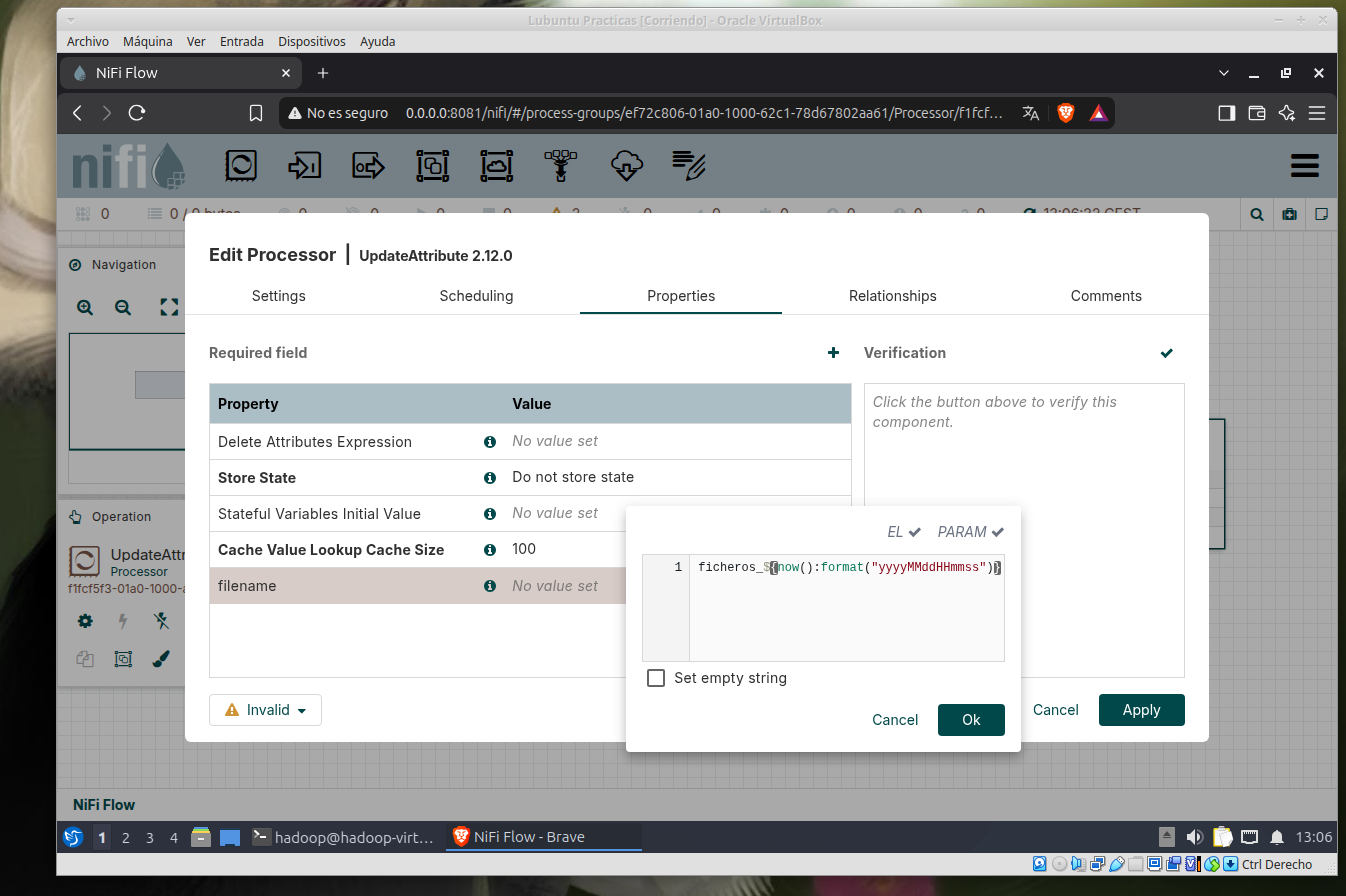
\includegraphics[width=0.8\textwidth]{50.png}
    \caption{Imagen 1}
    \label{fig:imagen1}
\end{figure}
\begin{figure}[ht]
    \centering
    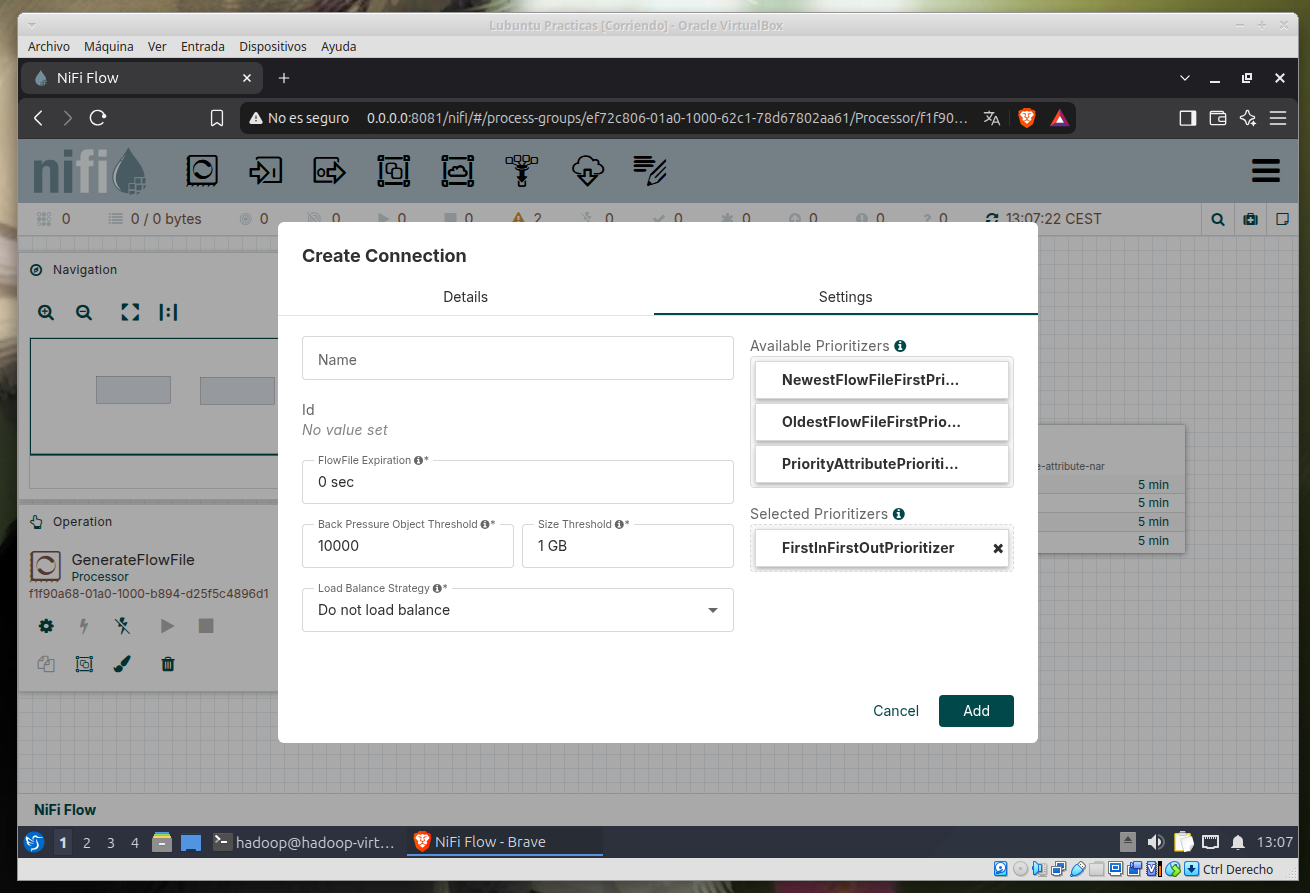
\includegraphics[width=0.8\textwidth]{51.png}
    \caption{Imagen 1}
    \label{fig:imagen1}
\end{figure}
\begin{figure}[ht]
    \centering
    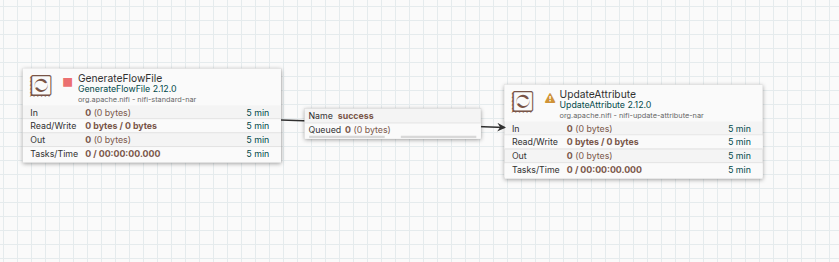
\includegraphics[width=0.8\textwidth]{52.png}
    \caption{Imagen 1}
    \label{fig:imagen1}
\end{figure}
\subsection{Creación de proceso de guardado}
\begin{figure}[ht]
    \centering
    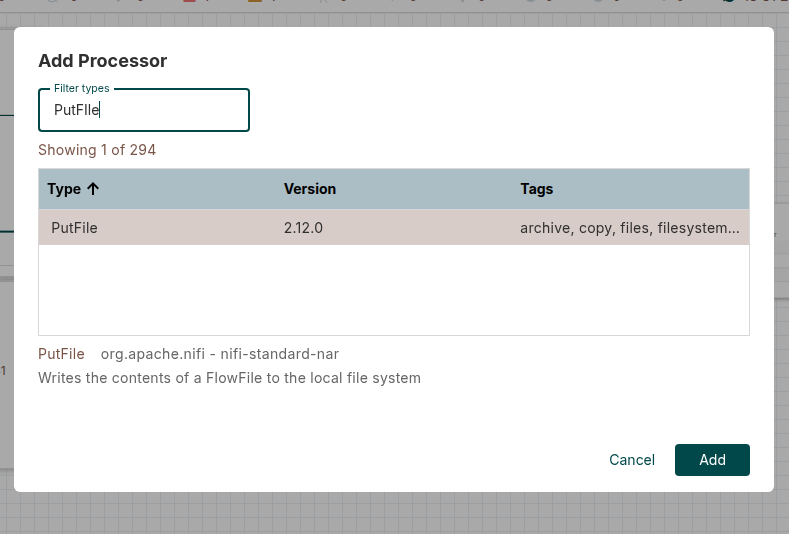
\includegraphics[width=0.8\textwidth]{53.png}
    \caption{Imagen 1}
    \label{fig:imagen1}
\end{figure}
\begin{figure}[ht]
    \centering
    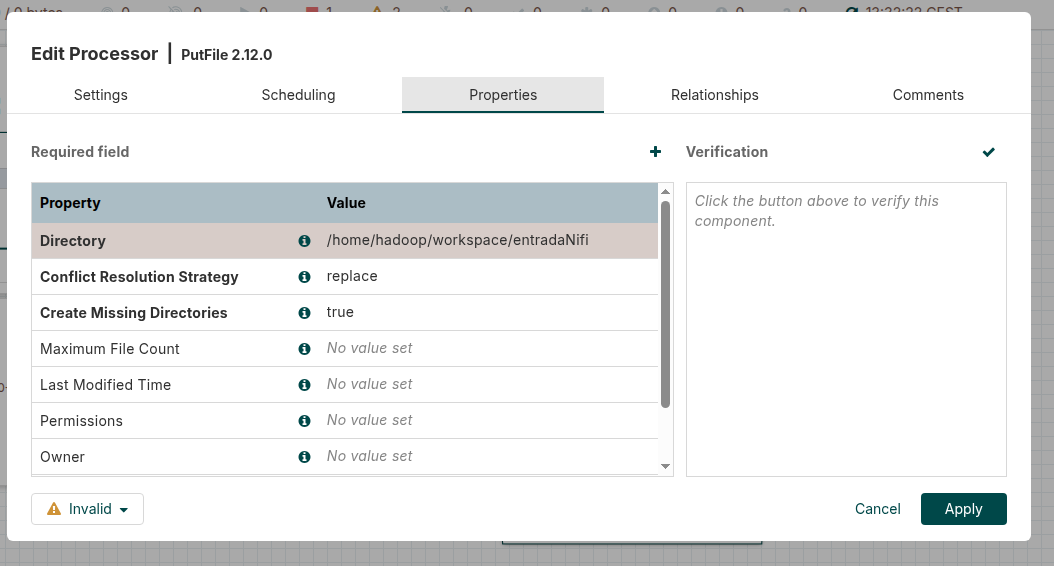
\includegraphics[width=0.8\textwidth]{54.png}
    \caption{Imagen 1}
    \label{fig:imagen1}
\end{figure}
\subsection{Uso de 'funnel'}
\begin{figure}[ht]
    \centering
    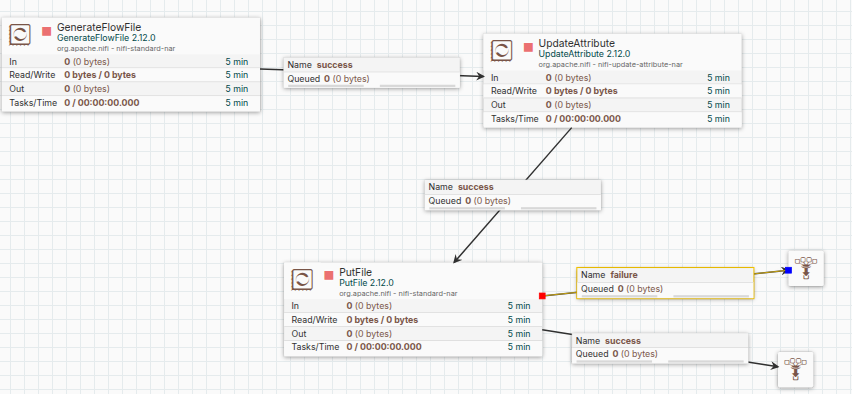
\includegraphics[width=0.8\textwidth]{57.png}
    \caption{Imagen 1}
    \label{fig:imagen1}
\end{figure}
\begin{figure}[ht]
    \centering
    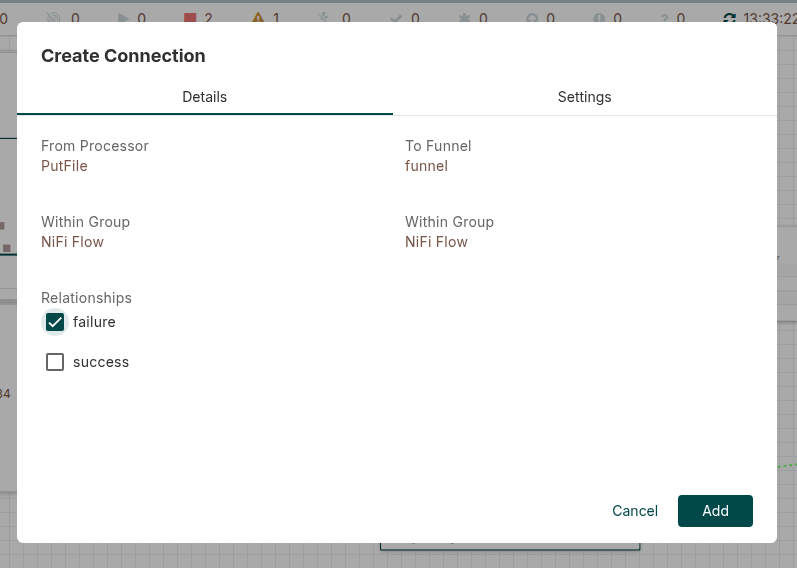
\includegraphics[width=0.8\textwidth]{55.png}
    \caption{Imagen 1}
    \label{fig:imagen1}
\end{figure}
\begin{figure}[ht]
    \centering
    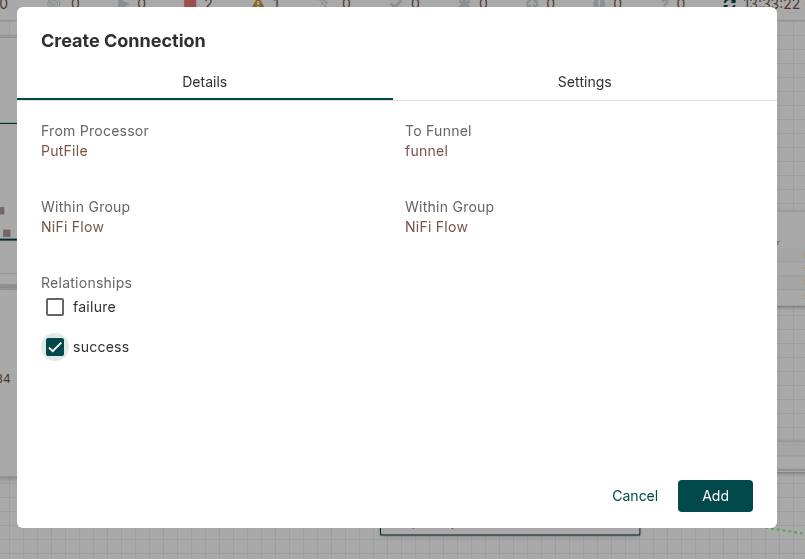
\includegraphics[width=0.8\textwidth]{56.png}
    \caption{Imagen 1}
    \label{fig:imagen1}
\end{figure}
\subsection{Prueba de flujo}
\begin{figure}[ht]
    \centering
    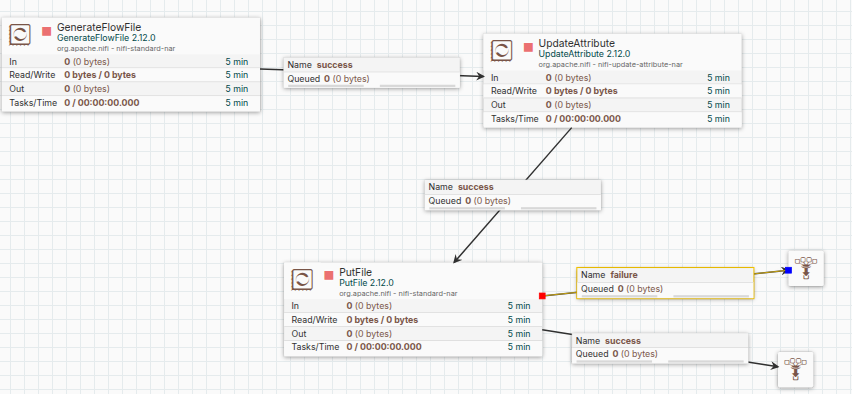
\includegraphics[width=0.8\textwidth]{57.png}
    \caption{Imagen 1}
    \label{fig:imagen1}
\end{figure}
\begin{figure}[ht]
    \centering
    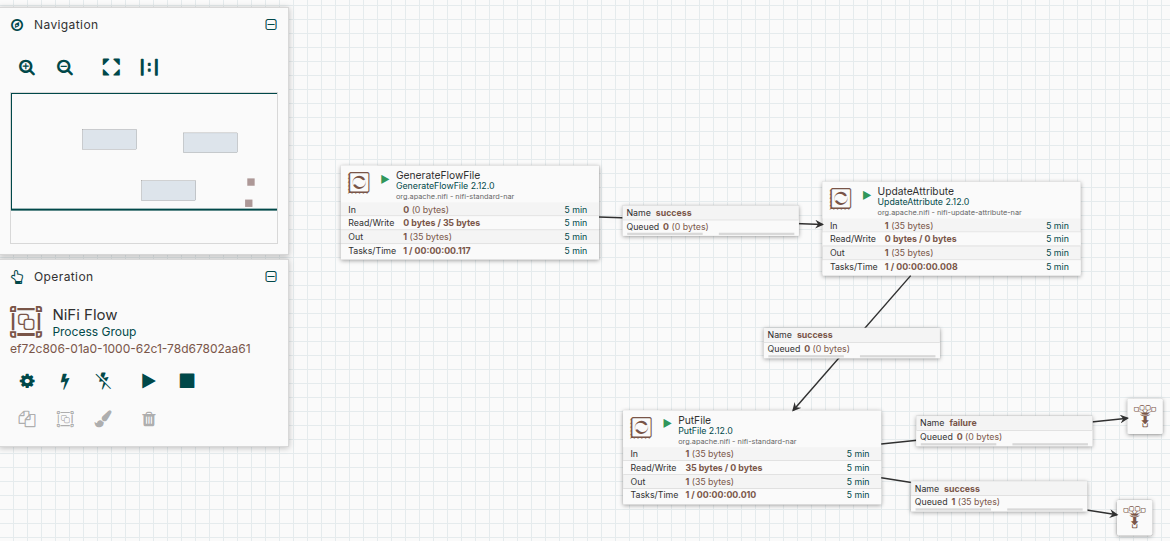
\includegraphics[width=0.8\textwidth]{58.png}
    \caption{Imagen 1}
    \label{fig:imagen1}
\end{figure}
\begin{figure}[ht]
    \centering
    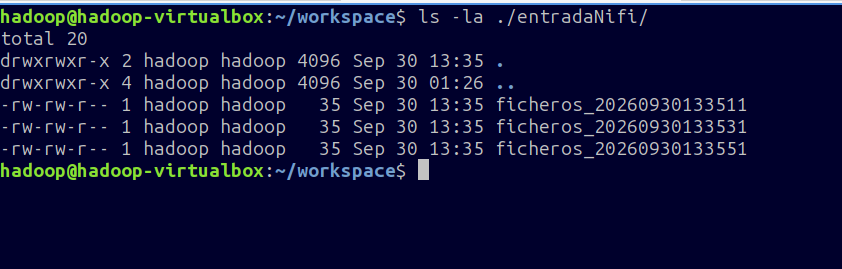
\includegraphics[width=0.8\textwidth]{59.png}
    \caption{Imagen 1}
    \label{fig:imagen1}
\end{figure}
\begin{figure}[ht]
    \centering
    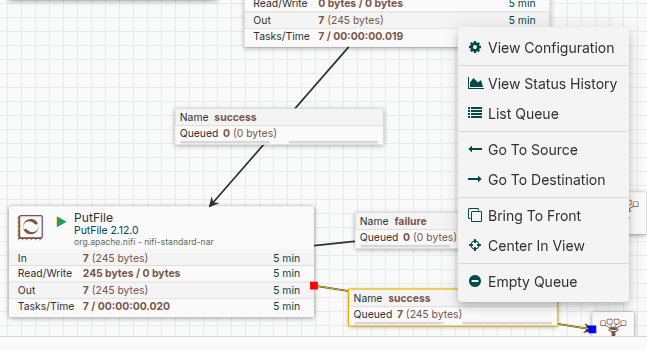
\includegraphics[width=0.8\textwidth]{60.png}
    \caption{Imagen 1}
    \label{fig:imagen1}
\end{figure}
\begin{figure}[ht]
    \centering
    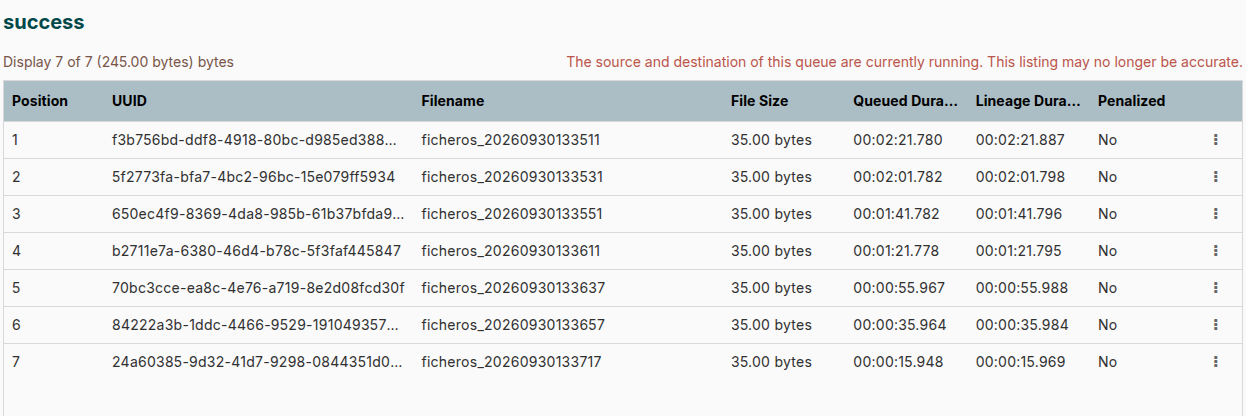
\includegraphics[width=0.8\textwidth]{61.png}
    \caption{Imagen 1}
    \label{fig:imagen1}
\end{figure}
\subsection{Creación de flujo de translado de ficheros}
\begin{figure}[ht]
    \centering
    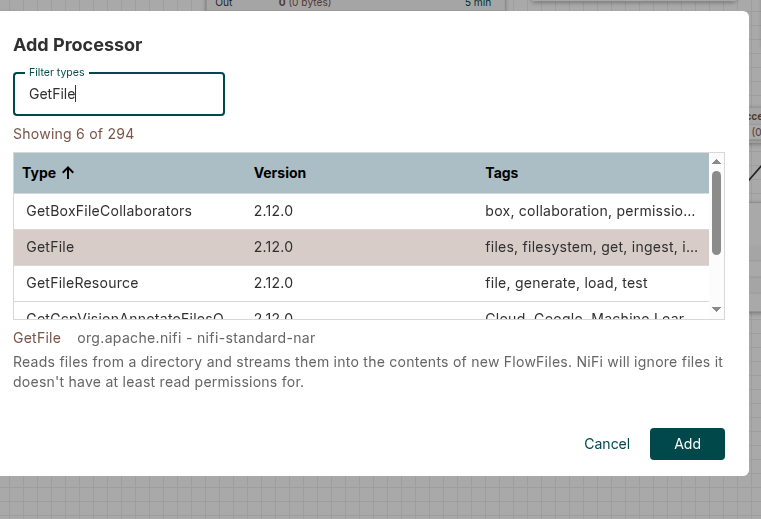
\includegraphics[width=0.8\textwidth]{62.png}
    \caption{Imagen 1}
    \label{fig:imagen1}
\end{figure}
\begin{figure}[ht]
    \centering
    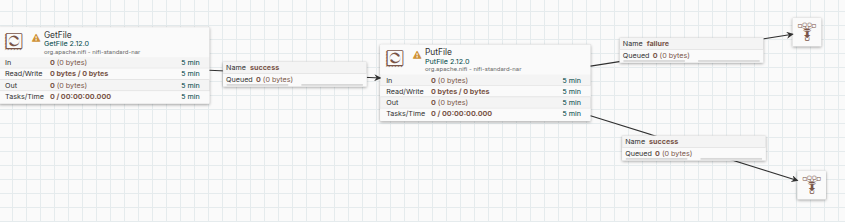
\includegraphics[width=0.8\textwidth]{63.png}
    \caption{Imagen 1}
    \label{fig:imagen1}
\end{figure}
\begin{figure}[ht]
    \centering
    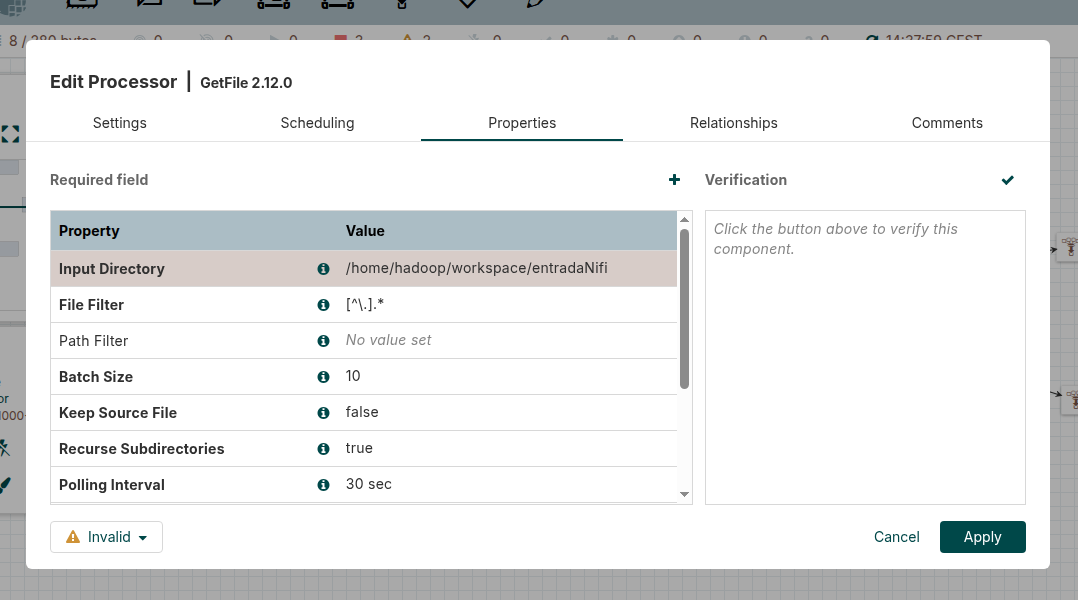
\includegraphics[width=0.8\textwidth]{64.png}
    \caption{Imagen 1}
    \label{fig:imagen1}
\end{figure}
\subsection{Prueba del nuevo flujo}
\begin{figure}[ht]
    \centering
    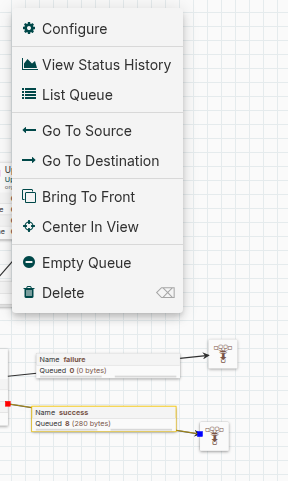
\includegraphics[width=0.8\textwidth]{65.png}
    \caption{Imagen 1}
    \label{fig:imagen1}
\end{figure}
\begin{figure}[ht]
    \centering
    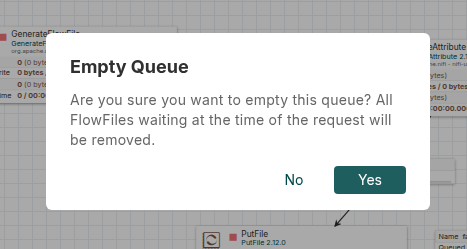
\includegraphics[width=0.8\textwidth]{66.png}
    \caption{Imagen 1}
    \label{fig:imagen1}
\end{figure}
\begin{figure}[ht]
    \centering
    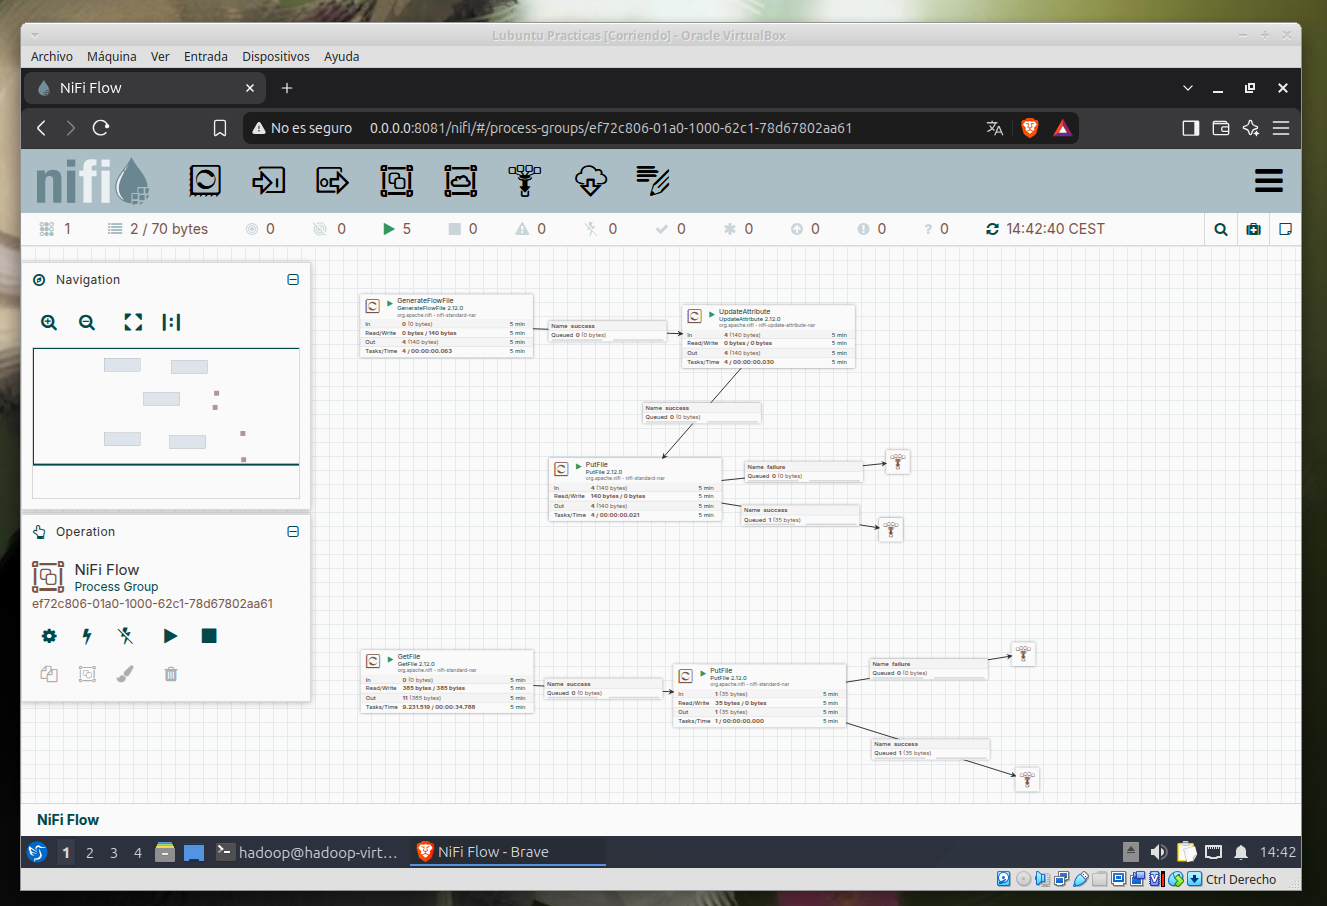
\includegraphics[width=0.8\textwidth]{67.png}
    \caption{Imagen 1}
    \label{fig:imagen1}
\end{figure}
\begin{figure}[ht]
    \centering
    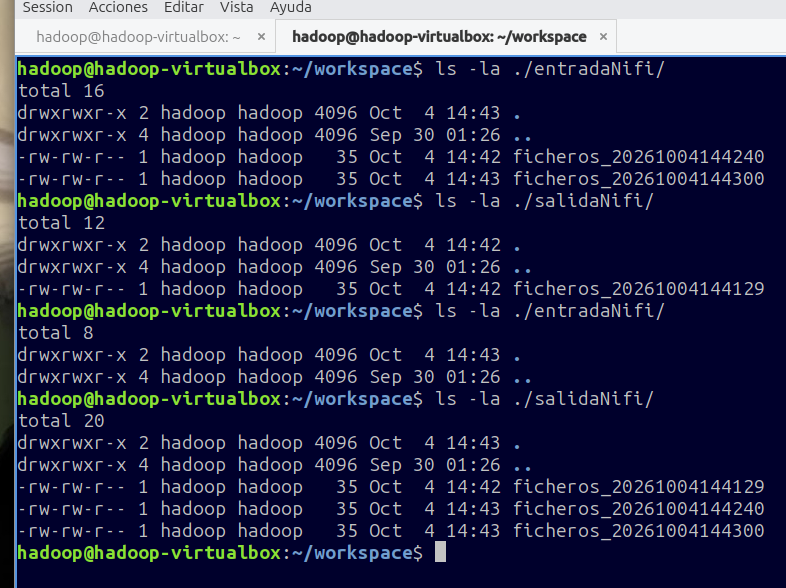
\includegraphics[width=0.8\textwidth]{68.png}
    \caption{Imagen 1}
    \label{fig:imagen1}
\end{figure}
\section{Practica 4 - Practicando con plantillas (grupos de procesos)}
\subsection{Creación de grupos y exportación}
\begin{figure}[ht]
    \centering
    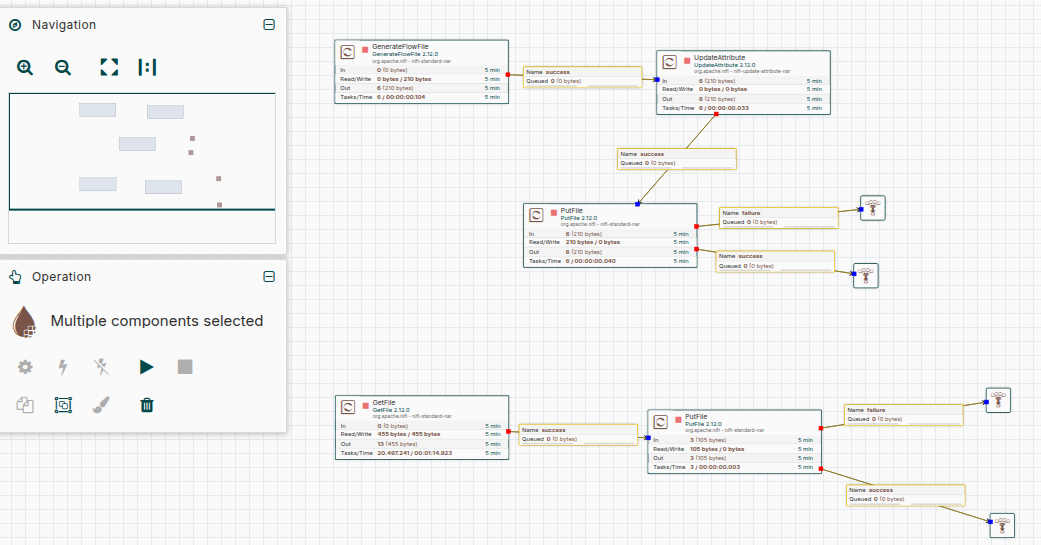
\includegraphics[width=0.8\textwidth]{69.png}
    \caption{Imagen 1}
    \label{fig:imagen1}
\end{figure}
\begin{figure}[ht]
    \centering
    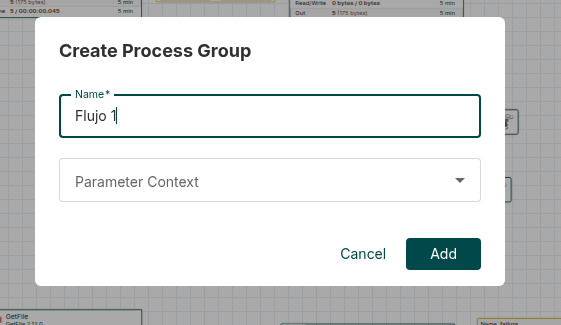
\includegraphics[width=0.8\textwidth]{70.png}
    \caption{Imagen 1}
    \label{fig:imagen1}
\end{figure}
\begin{figure}[ht]
    \centering
    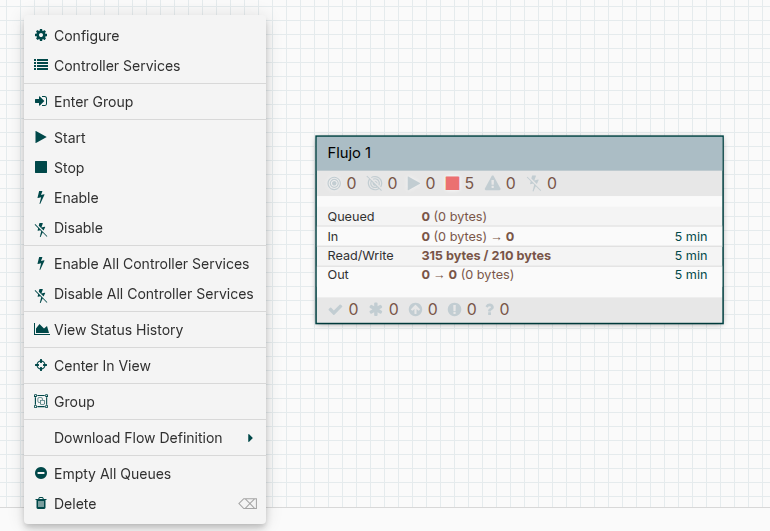
\includegraphics[width=0.8\textwidth]{71.png}
    \caption{Imagen 1}
    \label{fig:imagen1}
\end{figure}
\begin{figure}[ht]
    \centering
    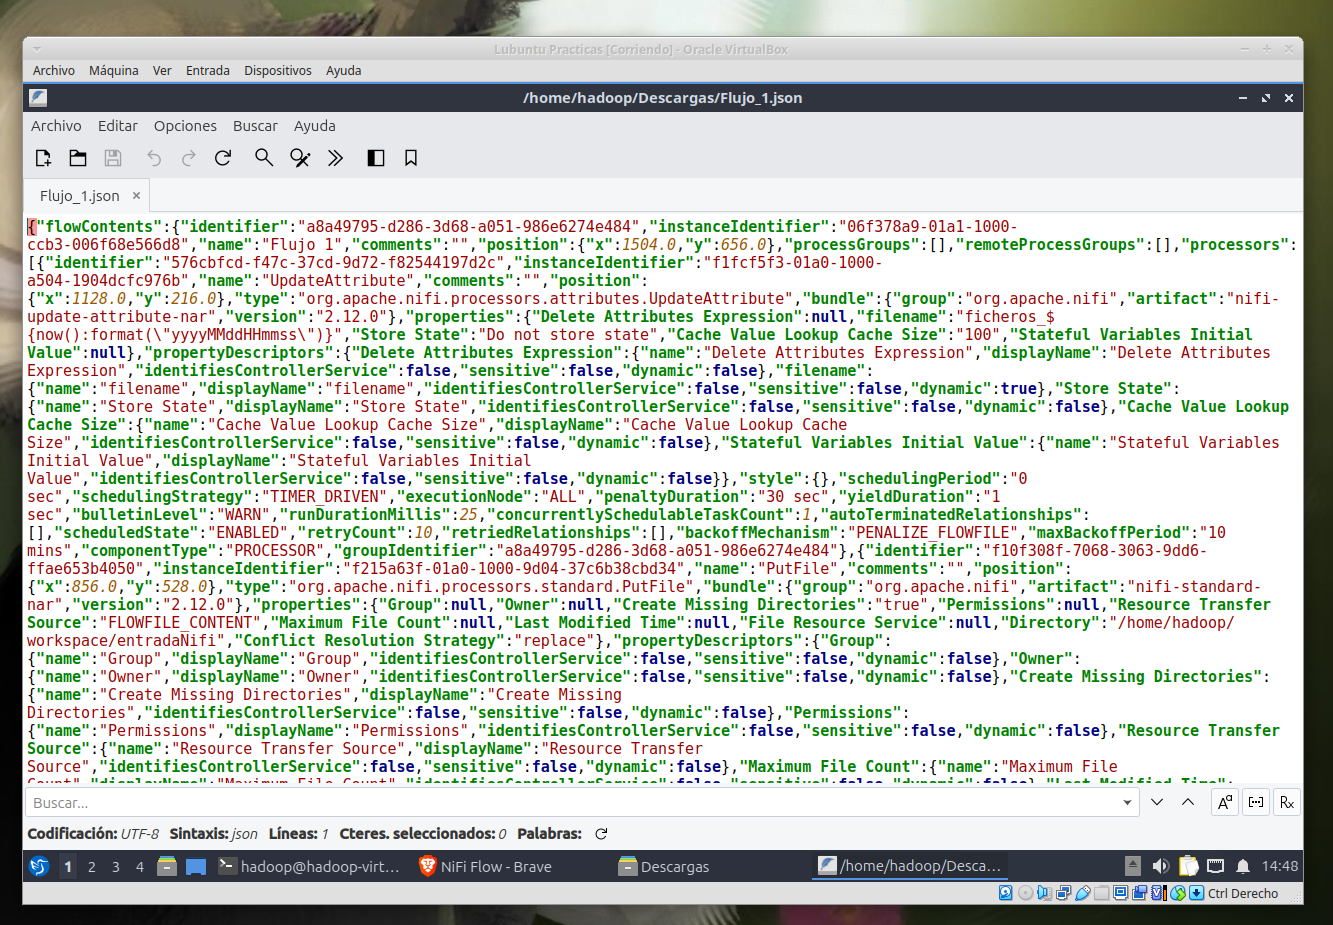
\includegraphics[width=0.8\textwidth]{72.png}
    \caption{Imagen 1}
    \label{fig:imagen1}
\end{figure}
\subsection{Cargar plantillas}
\begin{figure}[ht]
    \centering
    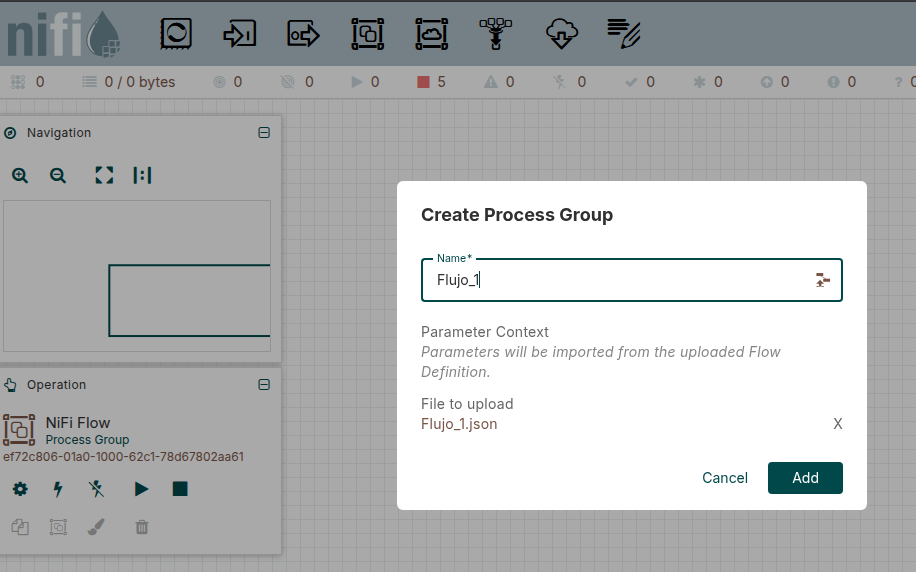
\includegraphics[width=0.8\textwidth]{73.png}
    \caption{Imagen 1}
    \label{fig:imagen1}
\end{figure}
\begin{figure}[ht]
    \centering
    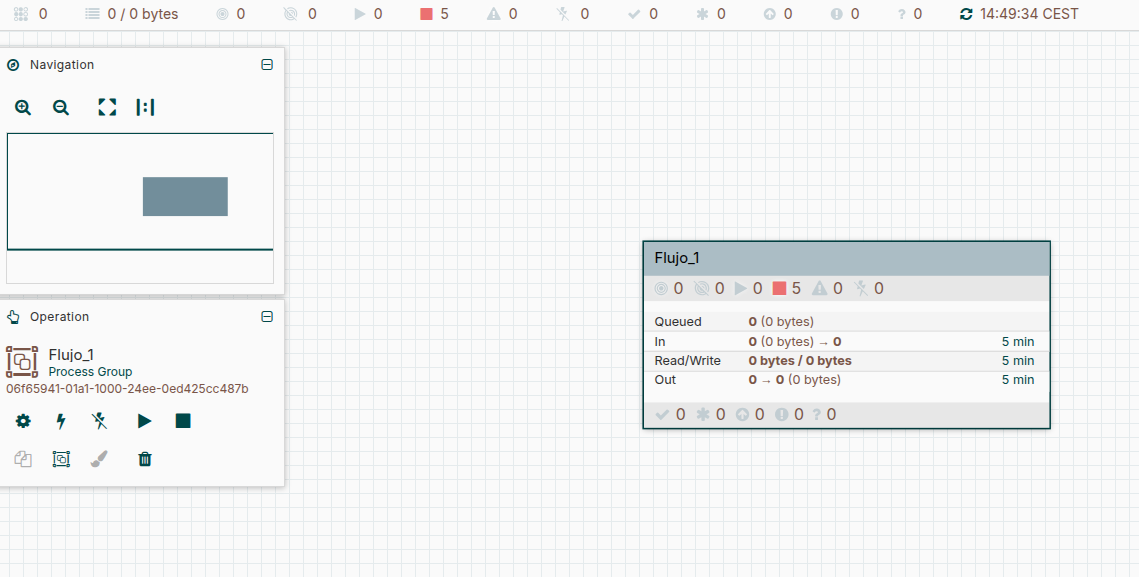
\includegraphics[width=0.8\textwidth]{74.png}
    \caption{Imagen 1}
    \label{fig:imagen1}
\end{figure}
\section{Practica 5 - Practicando con grupos de procesos}
\subsection{Creación del grupo de generación de ficheros}
\begin{figure}[ht]
    \centering
    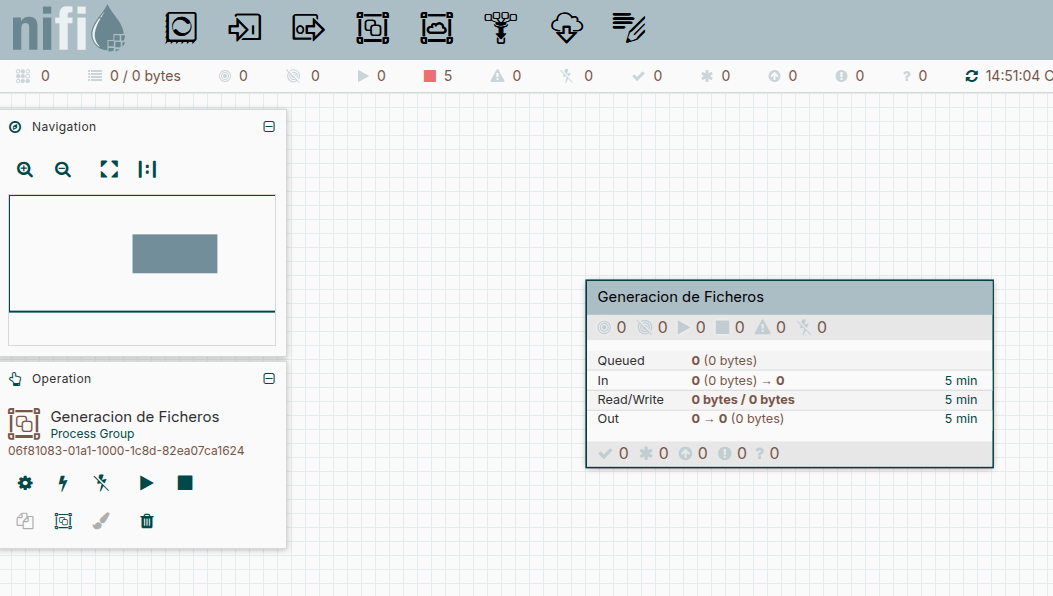
\includegraphics[width=0.8\textwidth]{75.png}
    \caption{Imagen 1}
    \label{fig:imagen1}
\end{figure}
\begin{figure}[ht]
    \centering
    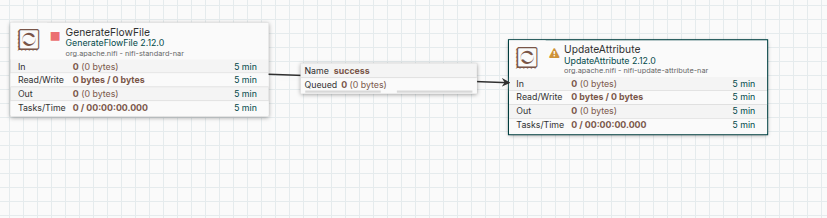
\includegraphics[width=0.8\textwidth]{76.png}
    \caption{Imagen 1}
    \label{fig:imagen1}
\end{figure}
\begin{figure}[ht]
    \centering
    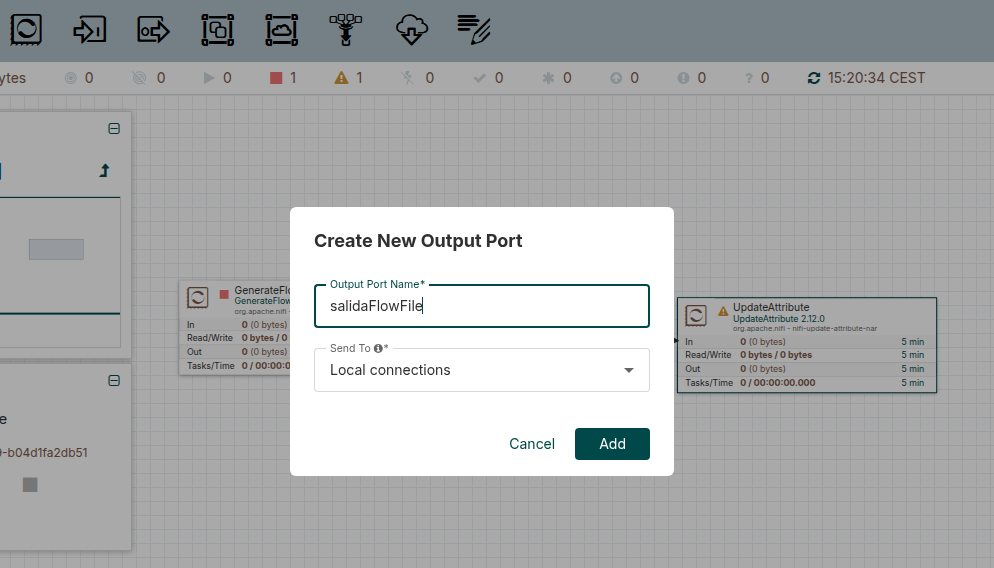
\includegraphics[width=0.8\textwidth]{77.png}
    \caption{Imagen 1}
    \label{fig:imagen1}
\end{figure}
\begin{figure}[ht]
    \centering
    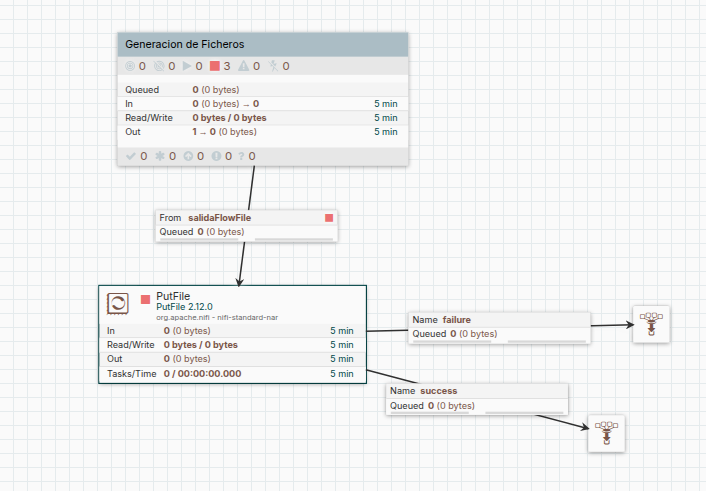
\includegraphics[width=0.8\textwidth]{79.png}
    \caption{Imagen 1}
    \label{fig:imagen1}
\end{figure}
\subsection{Añadir salida al grupo}
\begin{figure}[ht]
    \centering
    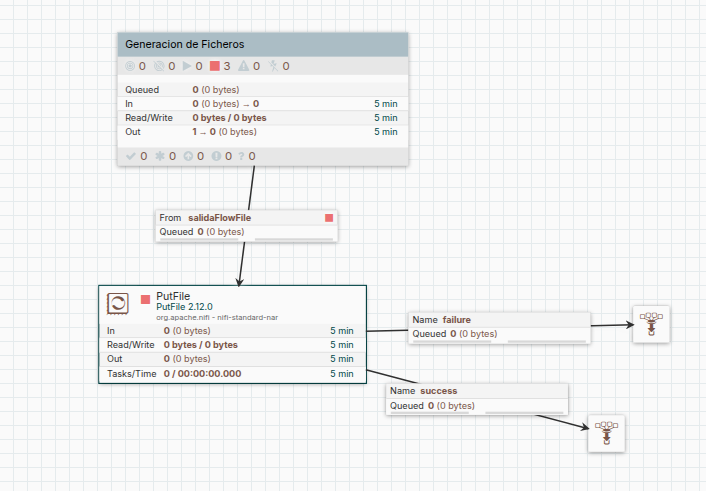
\includegraphics[width=0.8\textwidth]{79.png}
    \caption{Imagen 1}
    \label{fig:imagen1}
\end{figure}
\subsection{Comprobación del flujo}
\begin{figure}[ht]
    \centering
    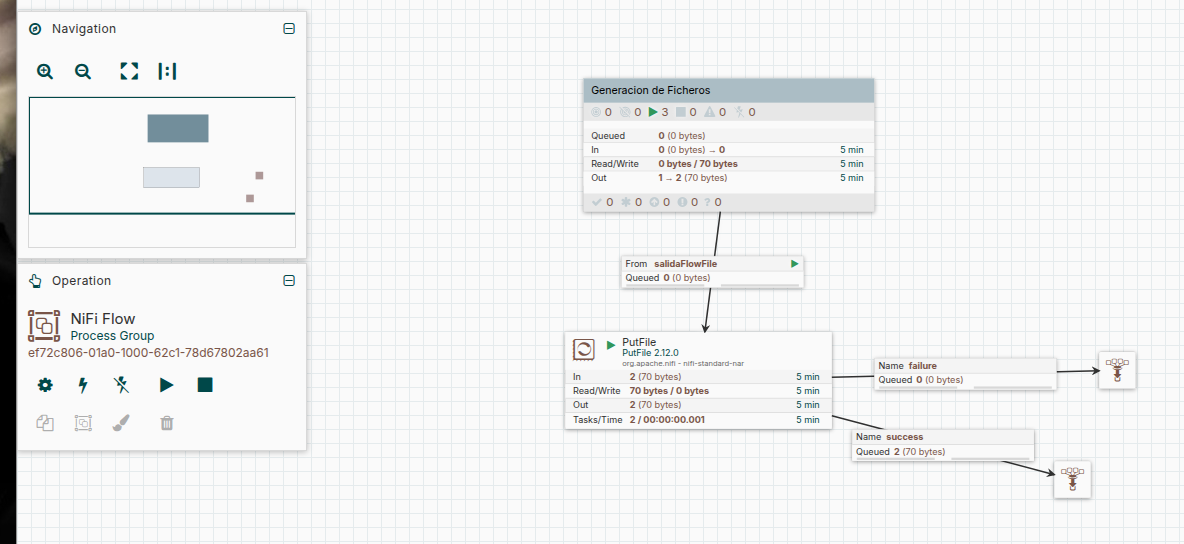
\includegraphics[width=0.8\textwidth]{80.png}
    \caption{Imagen 1}
    \label{fig:imagen1}
\end{figure}
\begin{figure}[ht]
    \centering
    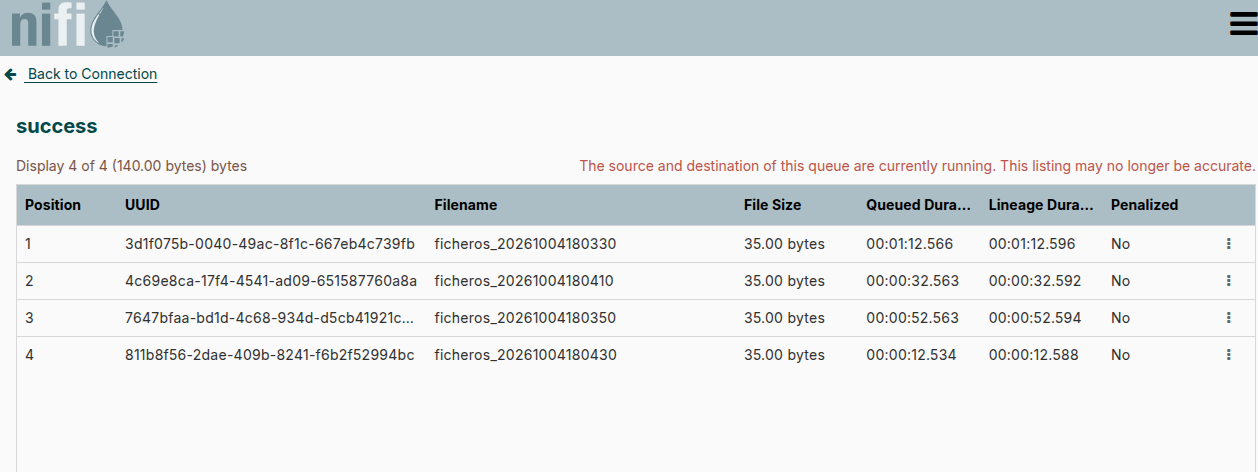
\includegraphics[width=0.8\textwidth]{81.png}
    \caption{Imagen 1}
    \label{fig:imagen1}
\end{figure}
\begin{figure}[ht]
    \centering
    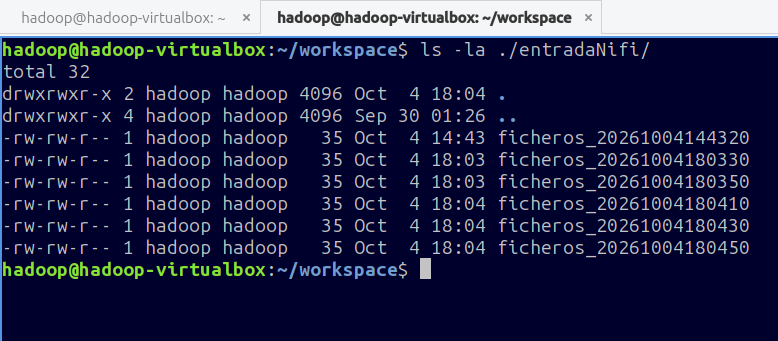
\includegraphics[width=0.8\textwidth]{82.png}
    \caption{Imagen 1}
    \label{fig:imagen1}
\end{figure}
\subsection{Creación del grupo para mover ficheros}
\begin{figure}[ht]
    \centering
    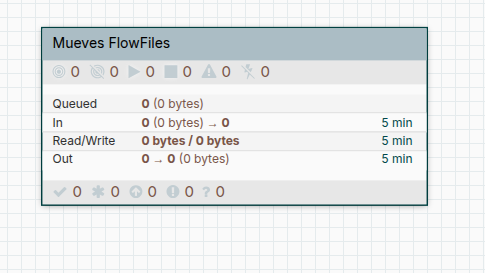
\includegraphics[width=0.8\textwidth]{83.png}
    \caption{Imagen 1}
    \label{fig:imagen1}
\end{figure}
\begin{figure}[ht]
    \centering
    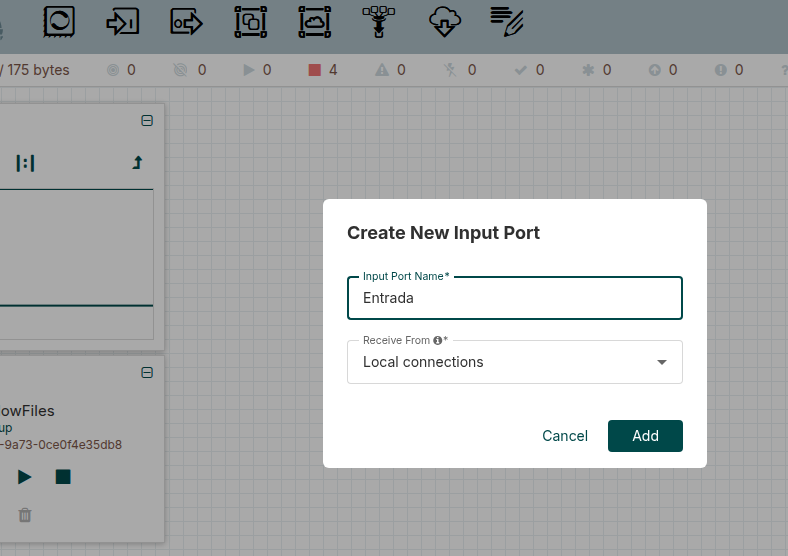
\includegraphics[width=0.8\textwidth]{84.png}
    \caption{Imagen 1}
    \label{fig:imagen1}
\end{figure}
\begin{figure}[ht]
    \centering
    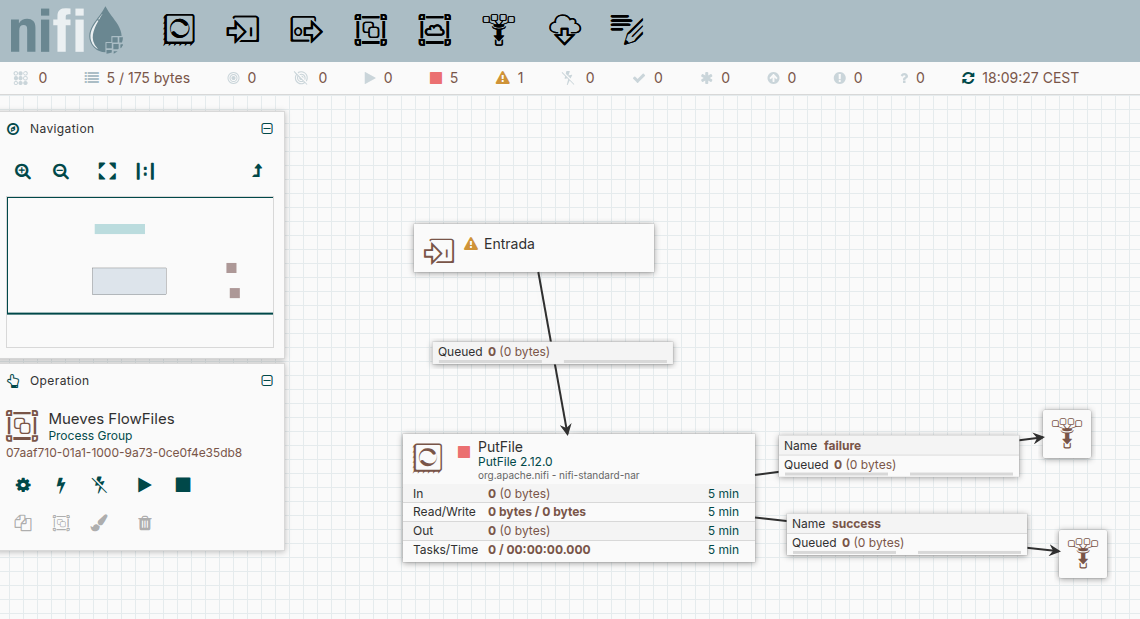
\includegraphics[width=0.8\textwidth]{85.png}
    \caption{Imagen 1}
    \label{fig:imagen1}
\end{figure}
\begin{figure}[ht]
    \centering
    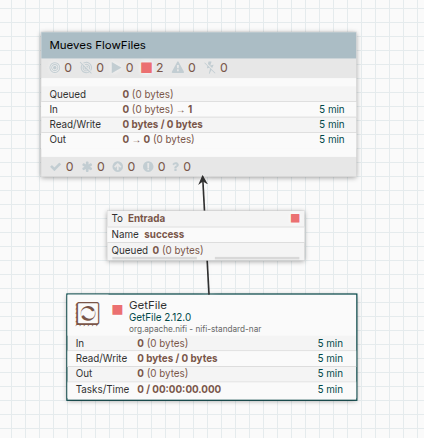
\includegraphics[width=0.8\textwidth]{86.png}
    \caption{Imagen 1}
    \label{fig:imagen1}
\end{figure}
\subsection{Comprobación del flujo}
\begin{figure}[ht]
    \centering
    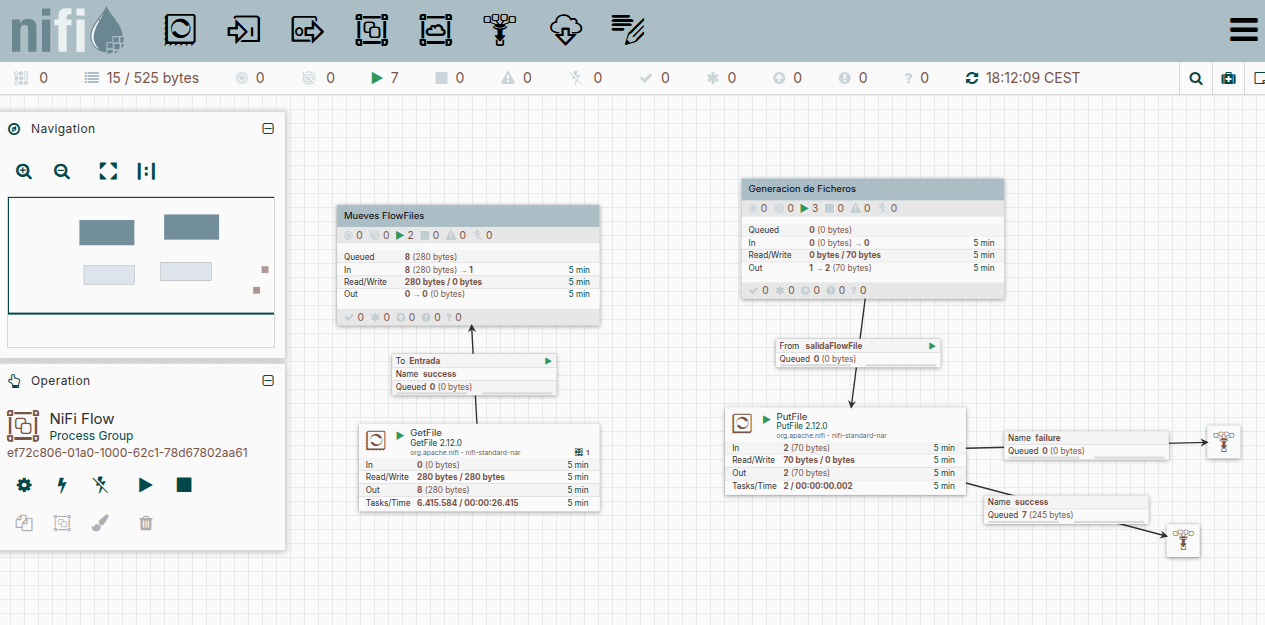
\includegraphics[width=0.8\textwidth]{87.png}
    \caption{Imagen 1}
    \label{fig:imagen1}
\end{figure}
\begin{figure}[ht]
    \centering
    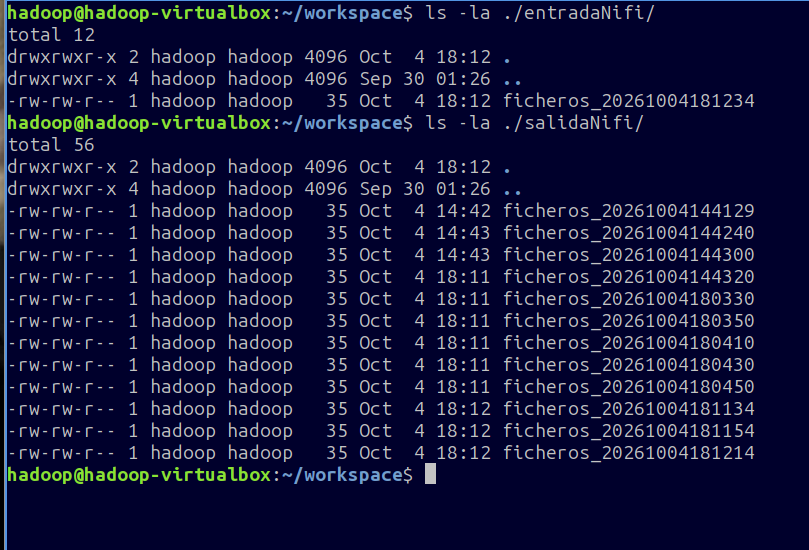
\includegraphics[width=0.8\textwidth]{88.png}
    \caption{Imagen 1}
    \label{fig:imagen1}
\end{figure}
\section{Practica 6 - Practicando la ingesta de datos en Batch}
\subsection{Instalación y configuración MySQL}
\begin{figure}[ht]
    \centering
    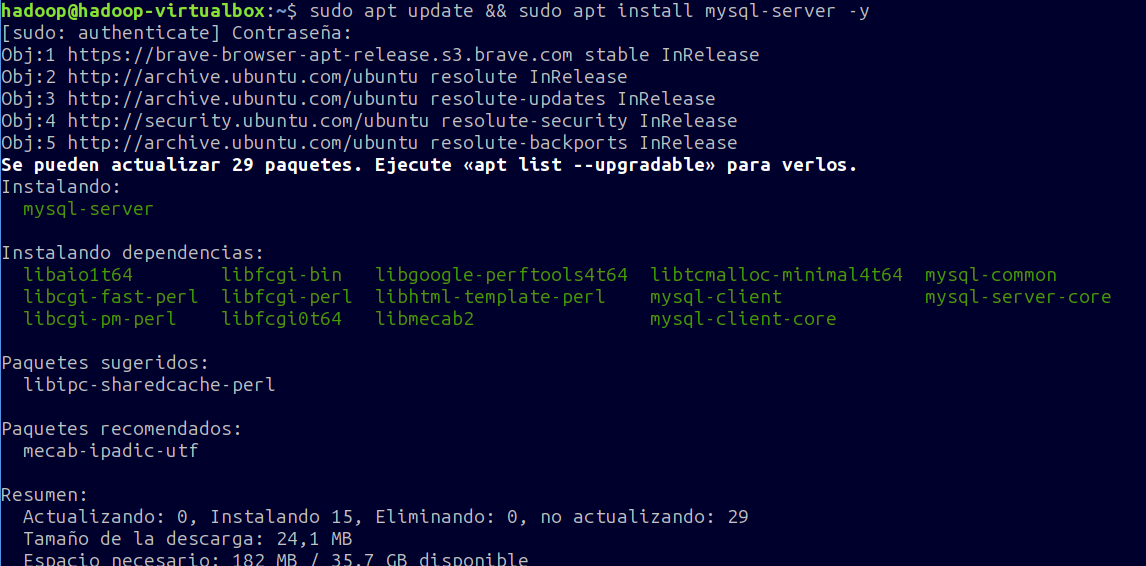
\includegraphics[width=0.8\textwidth]{89.png}
    \caption{Imagen 1}
    \label{fig:imagen1}
\end{figure}
\begin{figure}[ht]
    \centering
    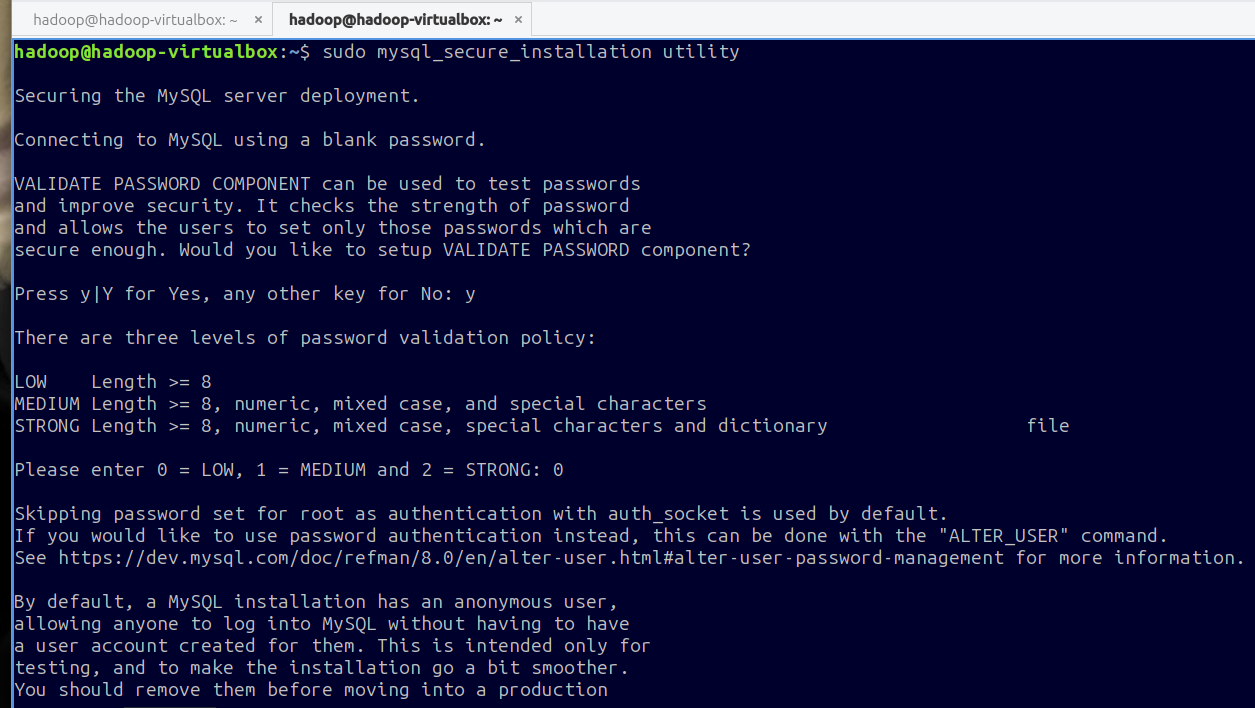
\includegraphics[width=0.8\textwidth]{90.png}
    \caption{Imagen 1}
    \label{fig:imagen1}
\end{figure}
\begin{figure}[ht]
    \centering
    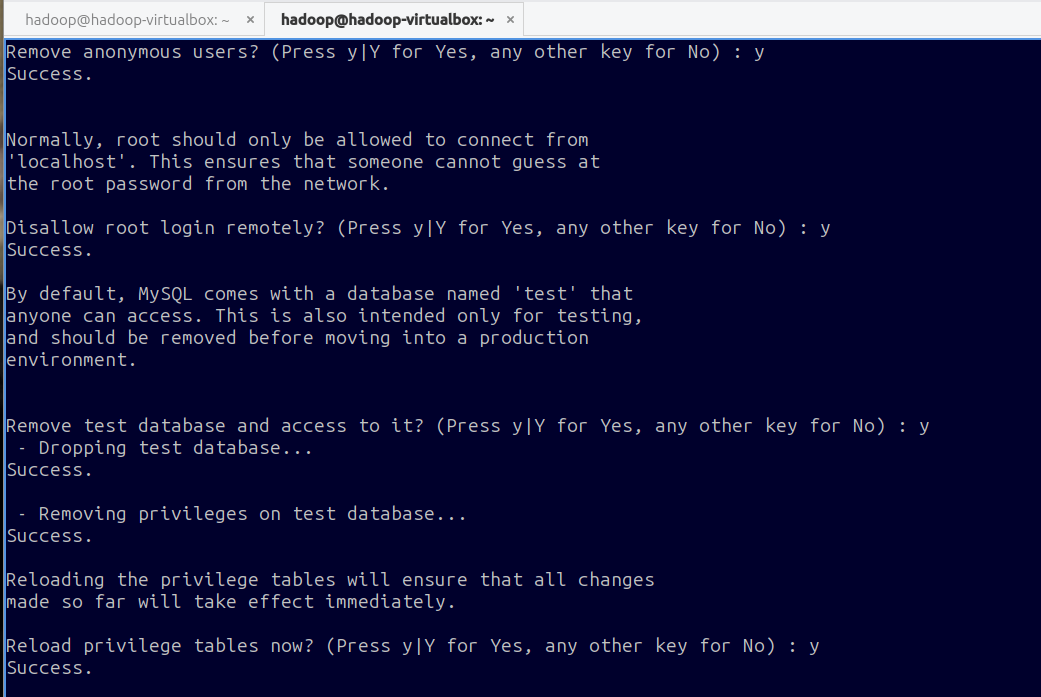
\includegraphics[width=0.8\textwidth]{91.png}
    \caption{Imagen 1}
    \label{fig:imagen1}
\end{figure}
\begin{figure}[ht]
    \centering
    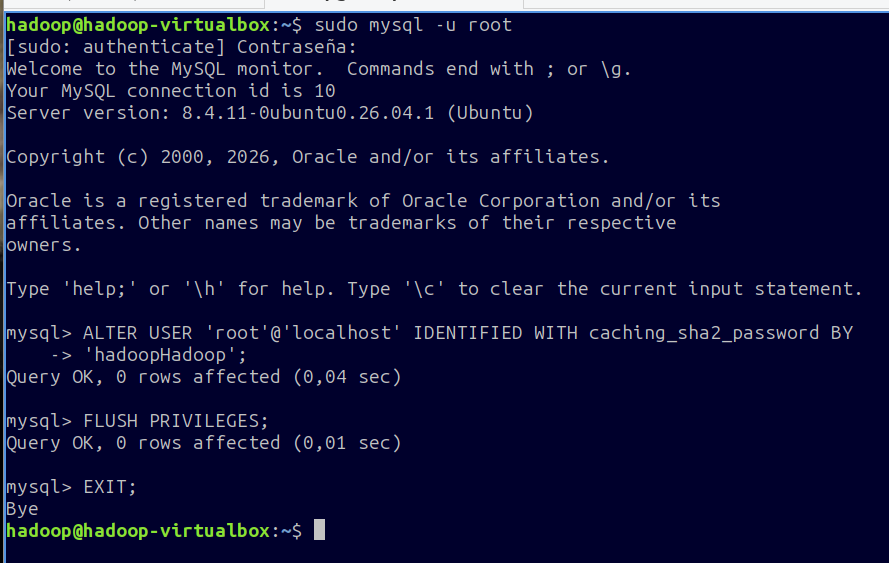
\includegraphics[width=0.8\textwidth]{92.png}
    \caption{Imagen 1}
    \label{fig:imagen1}
\end{figure}
\begin{figure}[ht]
    \centering
    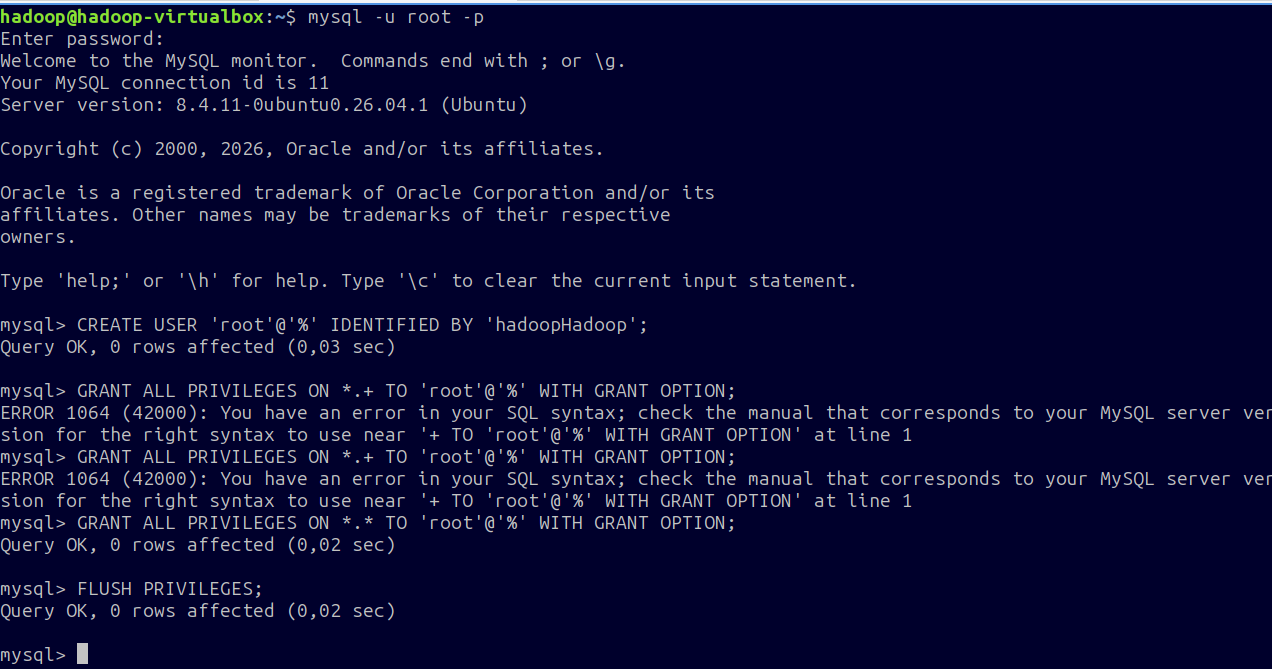
\includegraphics[width=0.8\textwidth]{93.png}
    \caption{Imagen 1}
    \label{fig:imagen1}
\end{figure}
\begin{figure}[ht]
    \centering
    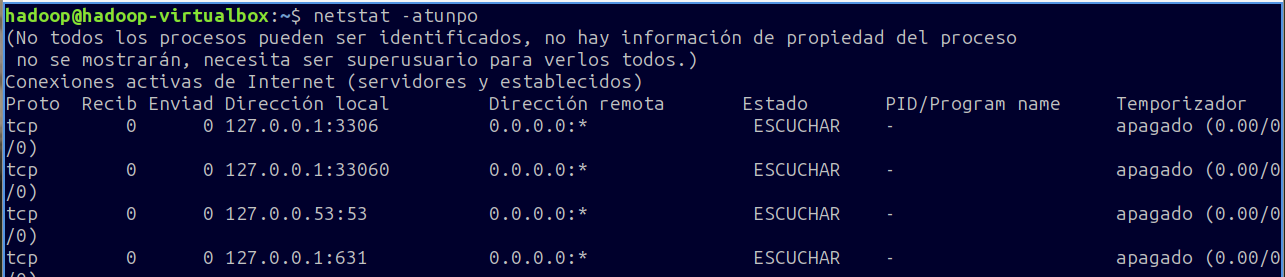
\includegraphics[width=0.8\textwidth]{94.png}
    \caption{Imagen 1}
    \label{fig:imagen1}
\end{figure}
\begin{figure}[ht]
    \centering
    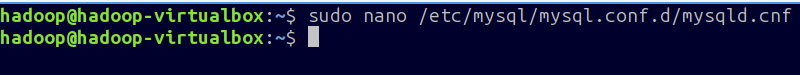
\includegraphics[width=0.8\textwidth]{95.png}
    \caption{Imagen 1}
    \label{fig:imagen1}
\end{figure}
\begin{figure}[ht]
    \centering
    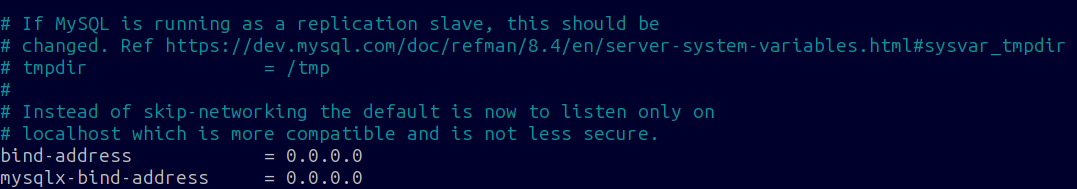
\includegraphics[width=0.8\textwidth]{96.png}
    \caption{Imagen 1}
    \label{fig:imagen1}
\end{figure}
\begin{figure}[ht]
    \centering
    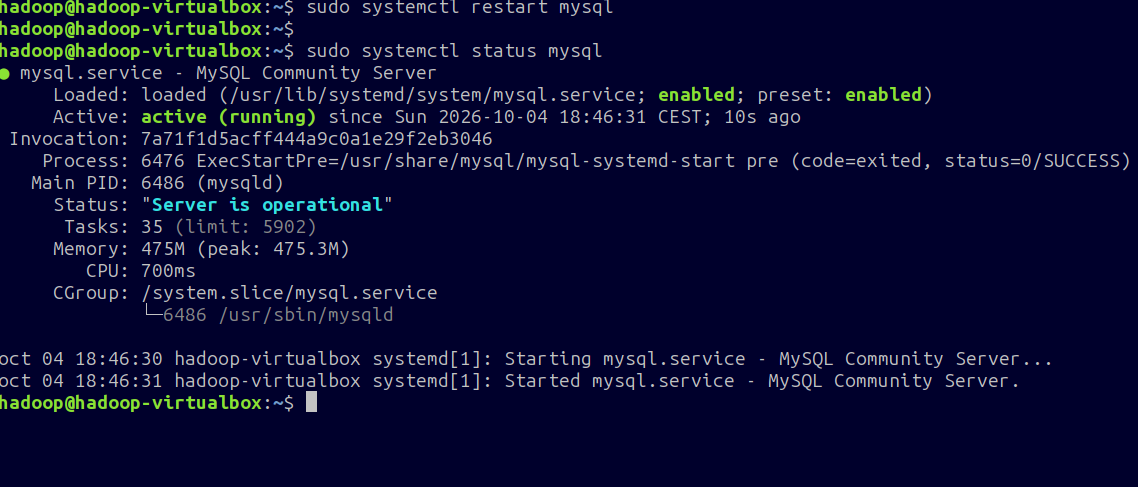
\includegraphics[width=0.8\textwidth]{97.png}
    \caption{Imagen 1}
    \label{fig:imagen1}
\end{figure}
\begin{figure}[ht]
    \centering
    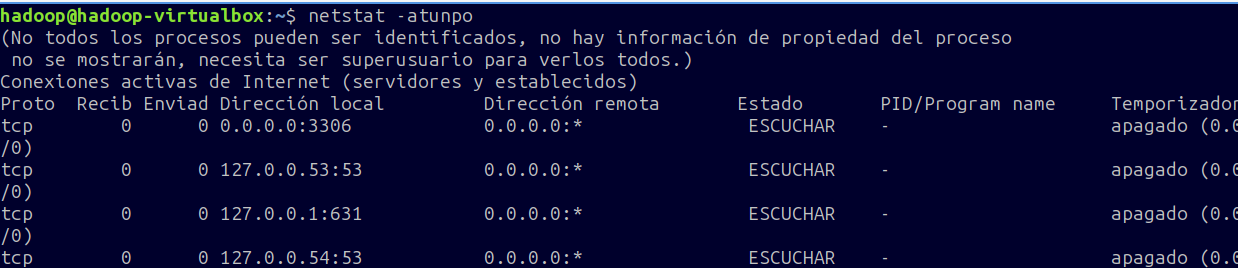
\includegraphics[width=0.8\textwidth]{98.png}
    \caption{Imagen 1}
    \label{fig:imagen1}
\end{figure}
\begin{figure}[ht]
    \centering
    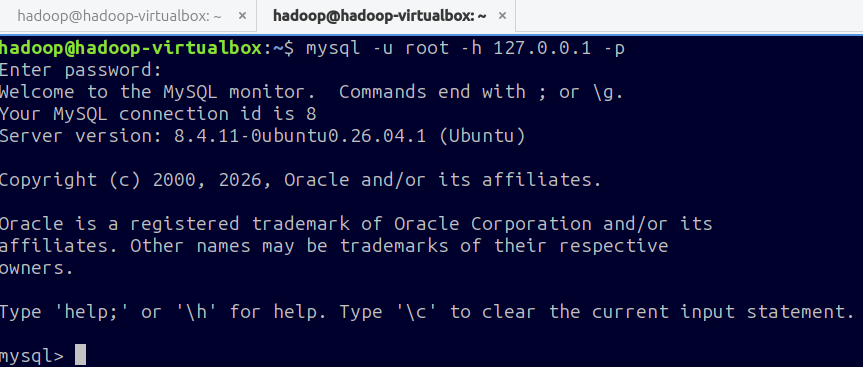
\includegraphics[width=0.8\textwidth]{99.png}
    \caption{Imagen 1}
    \label{fig:imagen1}
\end{figure}
\subsection{Creación de la Base de datos}
\begin{figure}[ht]
    \centering
    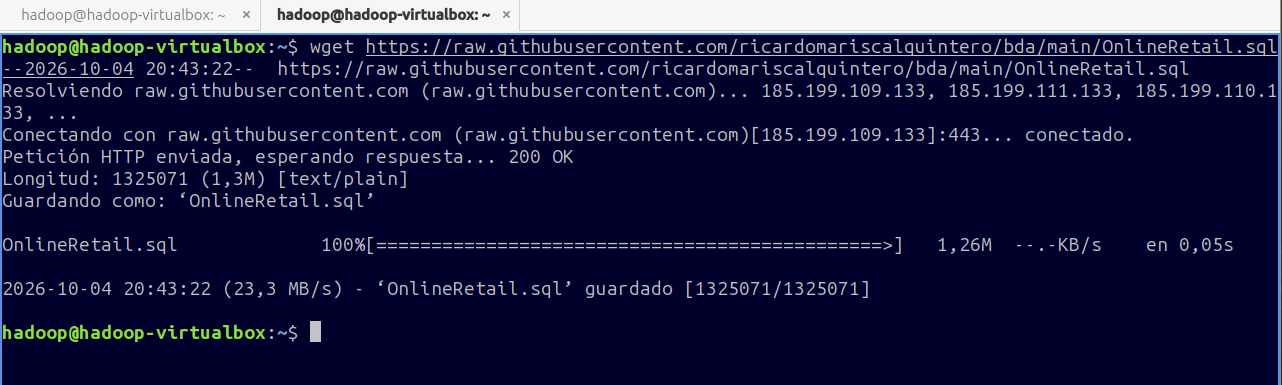
\includegraphics[width=0.8\textwidth]{100.png}
    \caption{Imagen 1}
    \label{fig:imagen1}
\end{figure}
\begin{figure}[ht]
    \centering
    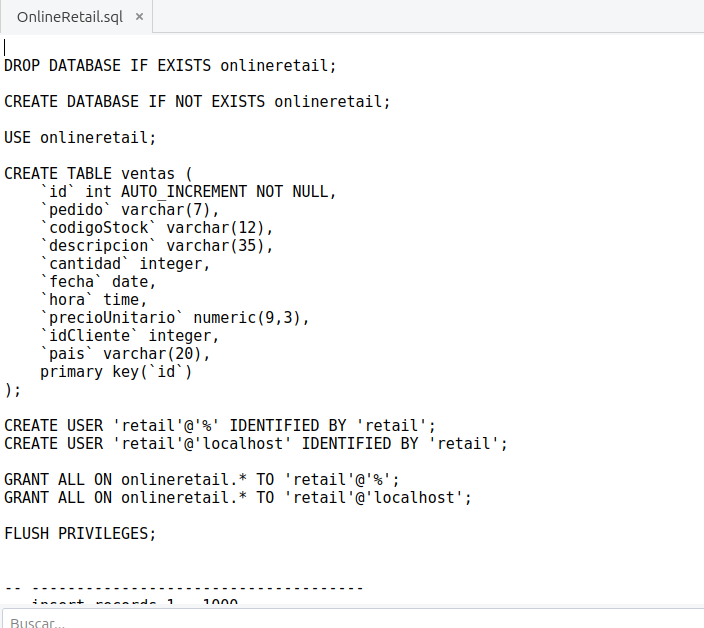
\includegraphics[width=0.8\textwidth]{101.png}
    \caption{Imagen 1}
    \label{fig:imagen1}
\end{figure}
\begin{figure}[ht]
    \centering
    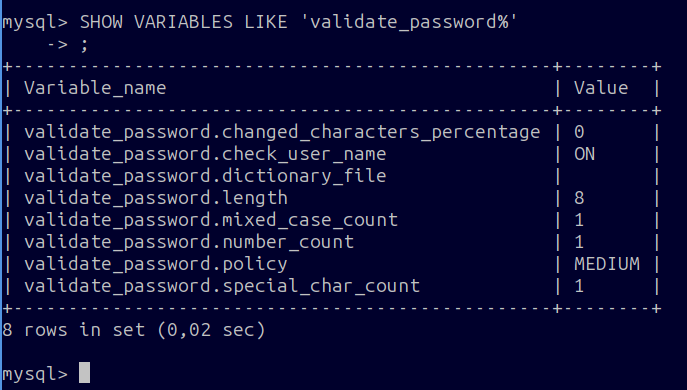
\includegraphics[width=0.8\textwidth]{102.png}
    \caption{Imagen 1}
    \label{fig:imagen1}
\end{figure}
\begin{figure}[ht]
    \centering
    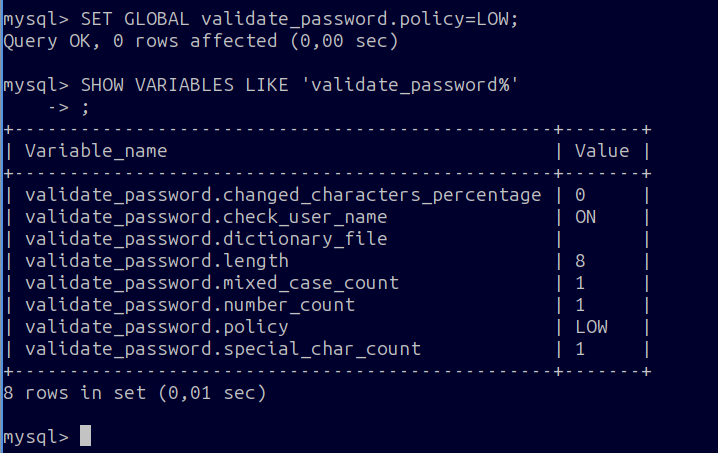
\includegraphics[width=0.8\textwidth]{103.png}
    \caption{Imagen 1}
    \label{fig:imagen1}
\end{figure}
\begin{figure}[ht]
    \centering
    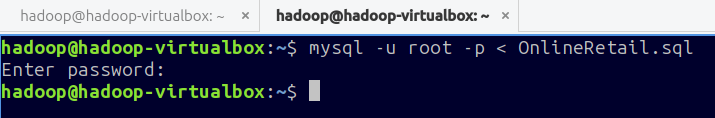
\includegraphics[width=0.8\textwidth]{104.png}
    \caption{Imagen 1}
    \label{fig:imagen1}
\end{figure}
\begin{figure}[ht]
    \centering
    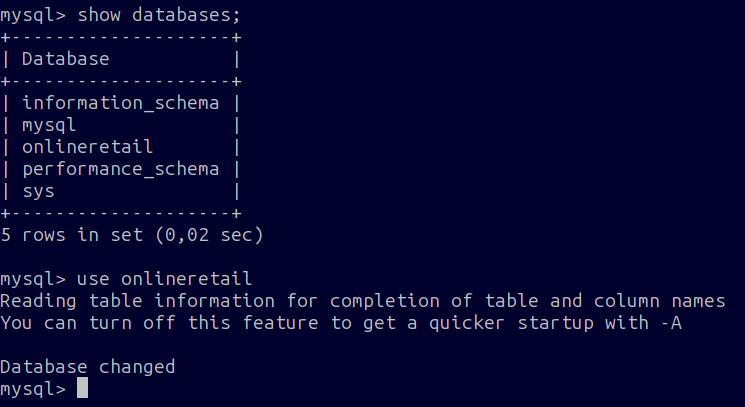
\includegraphics[width=0.8\textwidth]{105.png}
    \caption{Imagen 1}
    \label{fig:imagen1}
\end{figure}
\begin{figure}[ht]
    \centering
    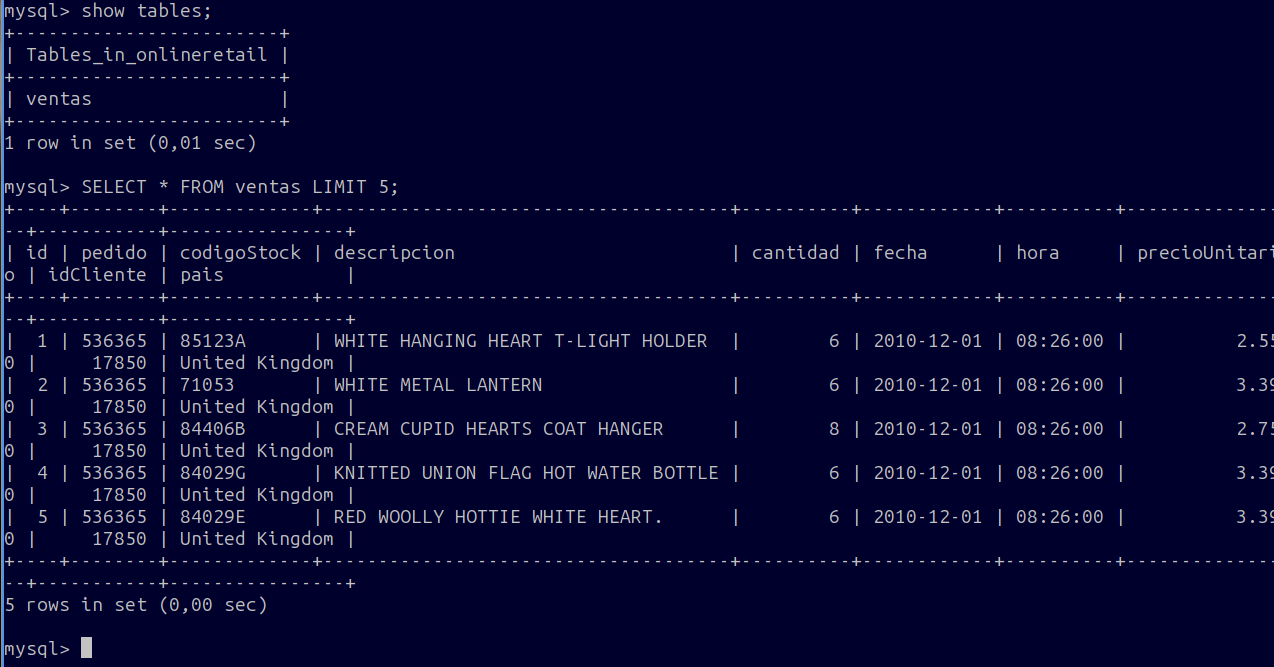
\includegraphics[width=0.8\textwidth]{106.png}
    \caption{Imagen 1}
    \label{fig:imagen1}
\end{figure}
\subsection{Descargamos la libreria de MySQL}
\begin{figure}[ht]
    \centering
    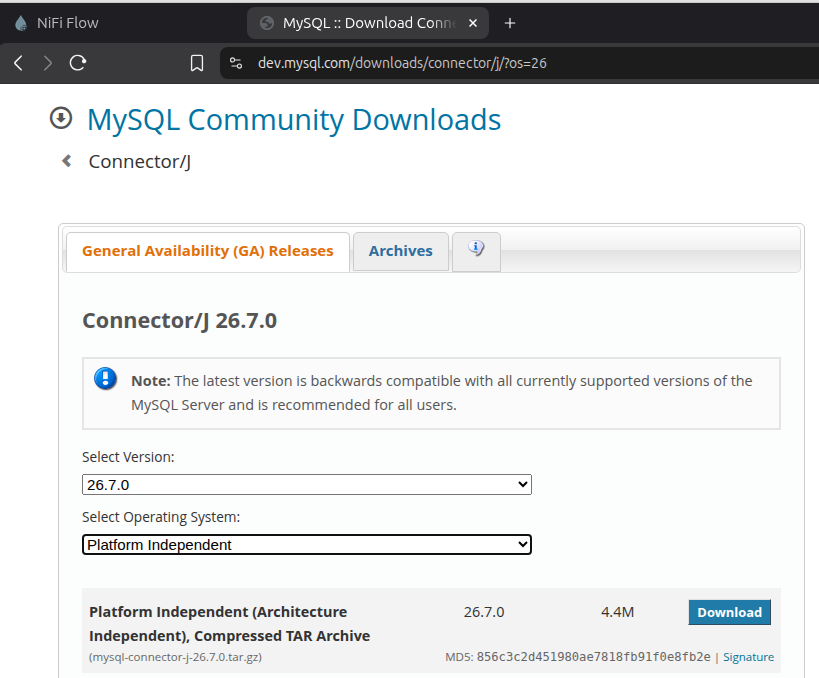
\includegraphics[width=0.8\textwidth]{107.png}
    \caption{Imagen 1}
    \label{fig:imagen1}
\end{figure}
\begin{figure}[ht]
    \centering
    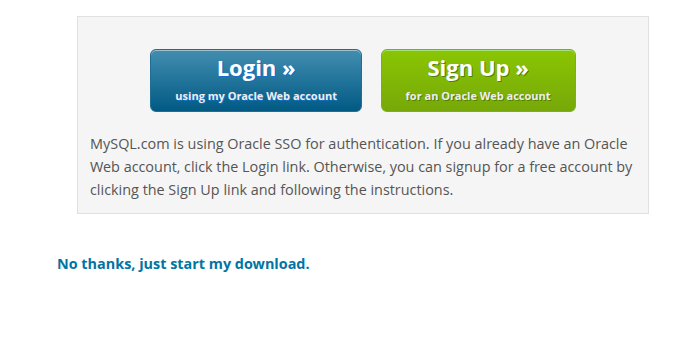
\includegraphics[width=0.8\textwidth]{108.png}
    \caption{Imagen 1}
    \label{fig:imagen1}
\end{figure}
\begin{figure}[ht]
    \centering
    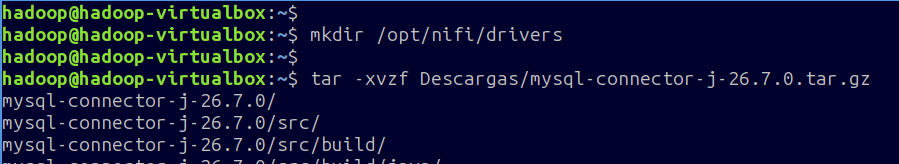
\includegraphics[width=0.8\textwidth]{109.png}
    \caption{Imagen 1}
    \label{fig:imagen1}
\end{figure}
\begin{figure}[ht]
    \centering
    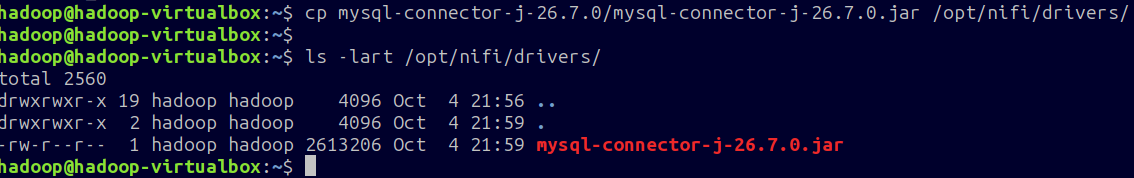
\includegraphics[width=0.8\textwidth]{110.png}
    \caption{Imagen 1}
    \label{fig:imagen1}
\end{figure}
\subsection{Damos de alta el servicio}
\begin{figure}[ht]
    \centering
    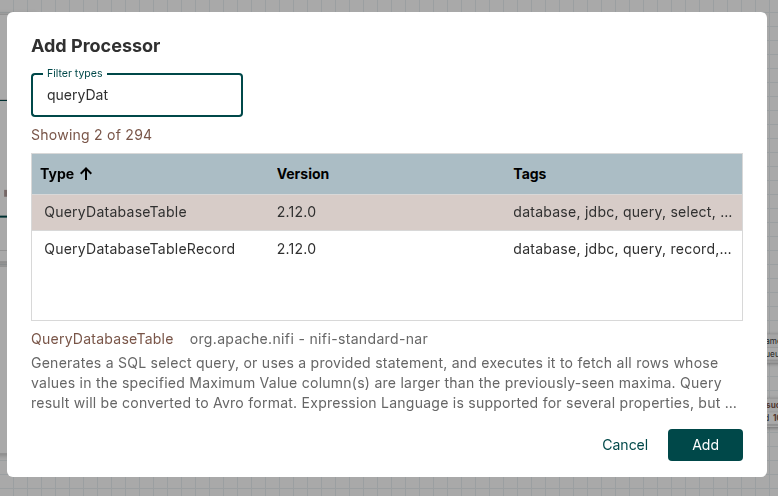
\includegraphics[width=0.8\textwidth]{111.png}
    \caption{Imagen 1}
    \label{fig:imagen1}
\end{figure}
\begin{figure}[ht]
    \centering
    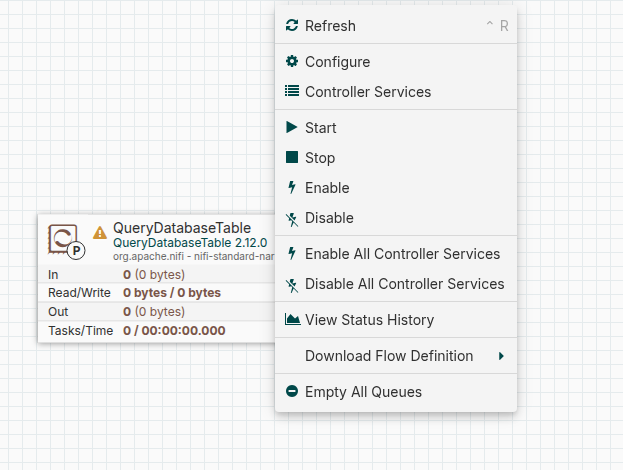
\includegraphics[width=0.8\textwidth]{112.png}
    \caption{Imagen 1}
    \label{fig:imagen1}
\end{figure}
\begin{figure}[ht]
    \centering
    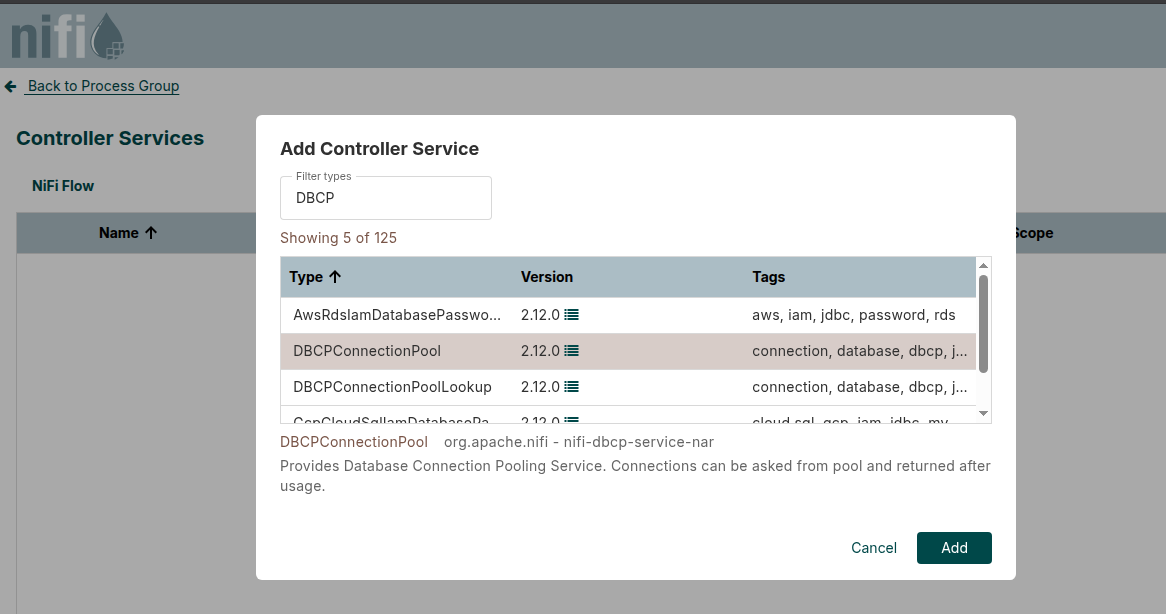
\includegraphics[width=0.8\textwidth]{113.png}
    \caption{Imagen 1}
    \label{fig:imagen1}
\end{figure}
\begin{figure}[ht]
    \centering
    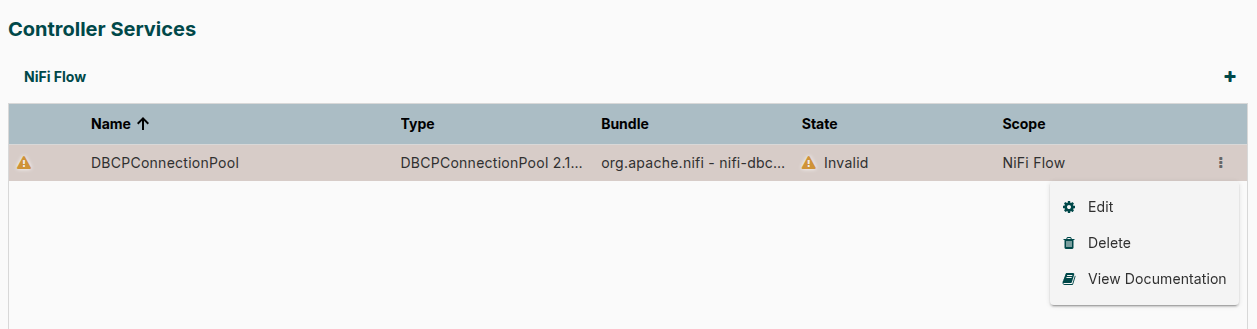
\includegraphics[width=0.8\textwidth]{114.png}
    \caption{Imagen 1}
    \label{fig:imagen1}
\end{figure}
\begin{figure}[ht]
    \centering
    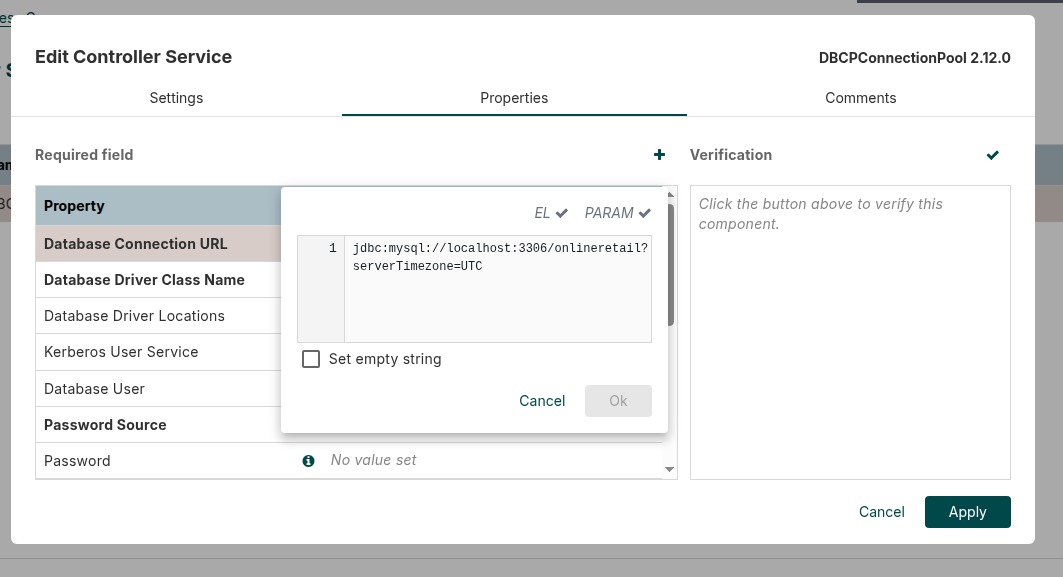
\includegraphics[width=0.8\textwidth]{115.png}
    \caption{Imagen 1}
    \label{fig:imagen1}
\end{figure}
\begin{figure}[ht]
    \centering
    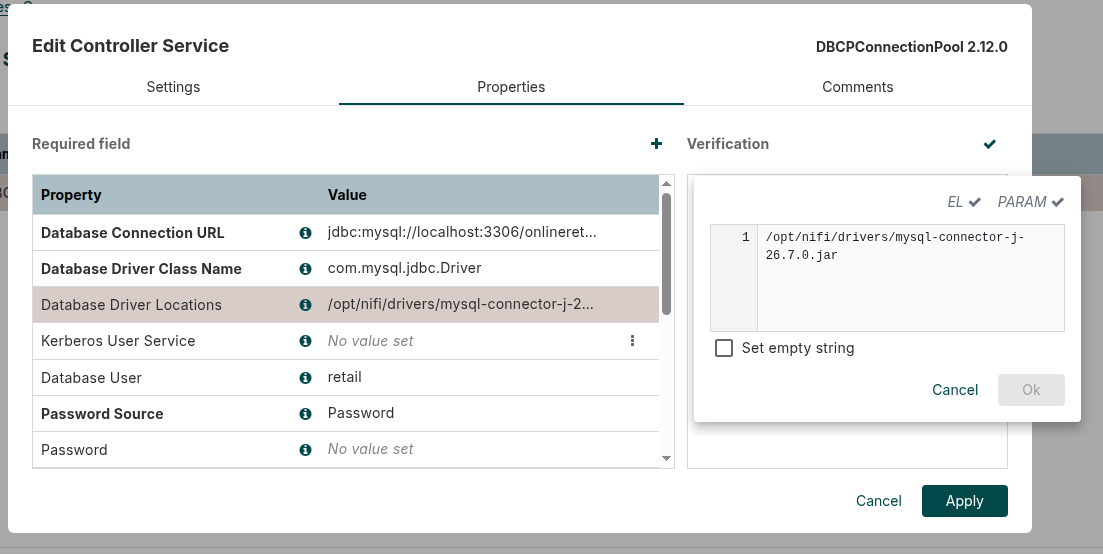
\includegraphics[width=0.8\textwidth]{116.png}
    \caption{Imagen 1}
    \label{fig:imagen1}
\end{figure}
\begin{figure}[ht]
    \centering
    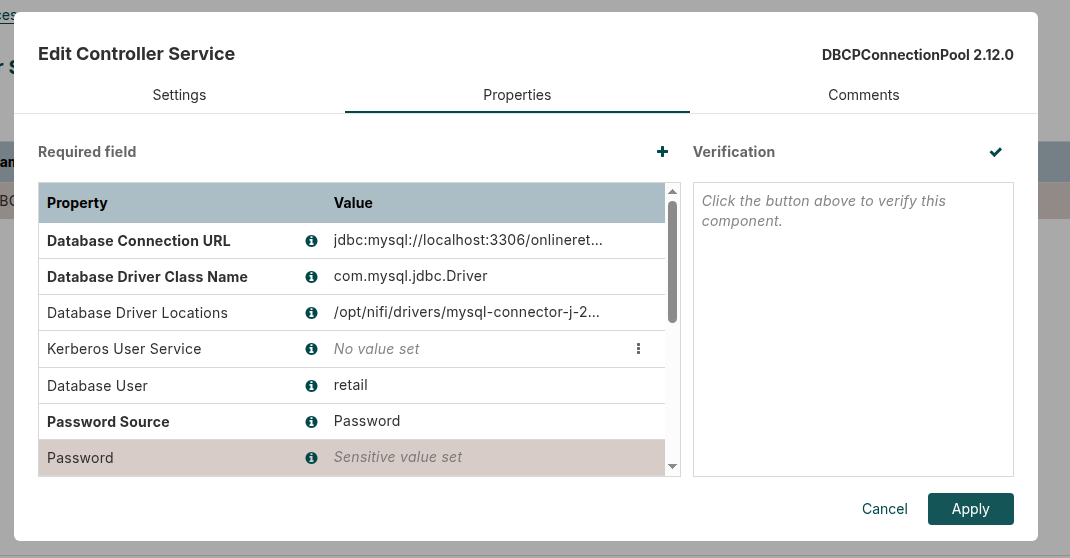
\includegraphics[width=0.8\textwidth]{117.png}
    \caption{Imagen 1}
    \label{fig:imagen1}
\end{figure}
\begin{figure}[ht]
    \centering
    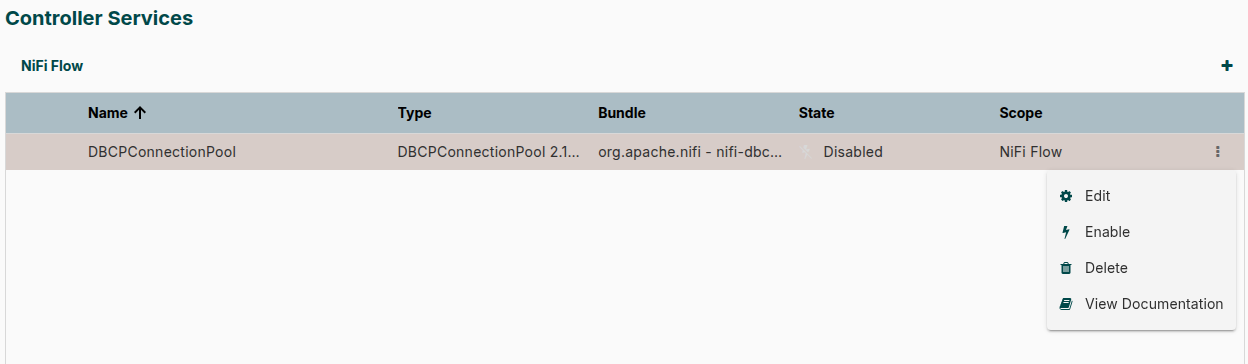
\includegraphics[width=0.8\textwidth]{118.png}
    \caption{Imagen 1}
    \label{fig:imagen1}
\end{figure}
\begin{figure}[ht]
    \centering
    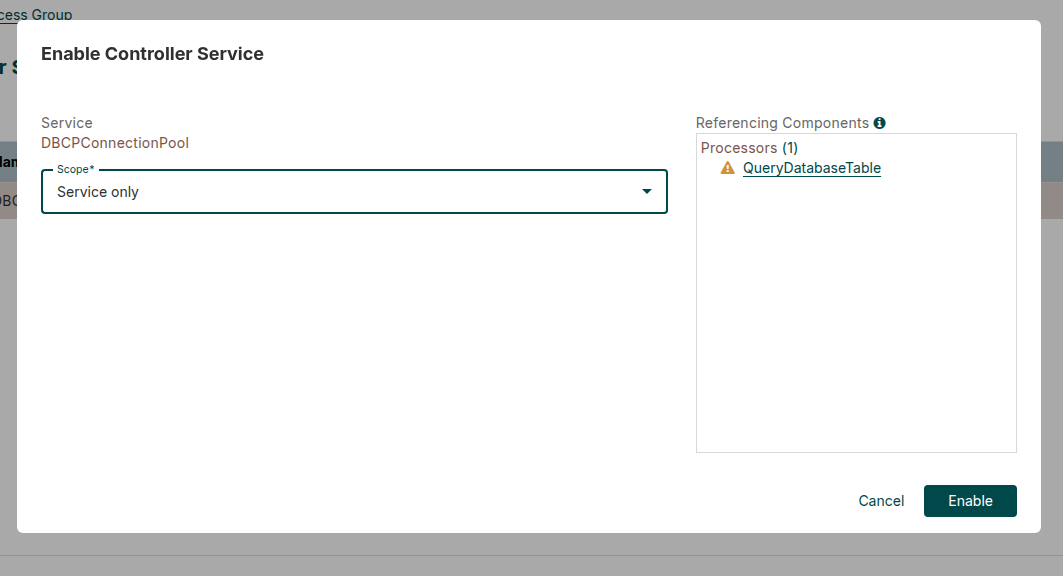
\includegraphics[width=0.8\textwidth]{119.png}
    \caption{Imagen 1}
    \label{fig:imagen1}
\end{figure}
\begin{figure}[ht]
    \centering
    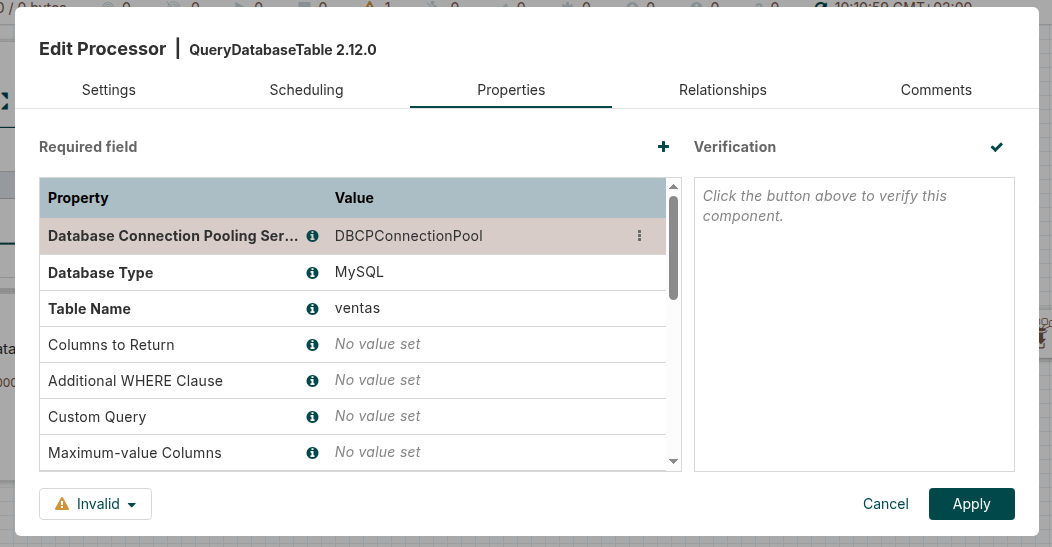
\includegraphics[width=0.8\textwidth]{120.png}
    \caption{Imagen 1}
    \label{fig:imagen1}
\end{figure}
\begin{figure}[ht]
    \centering
    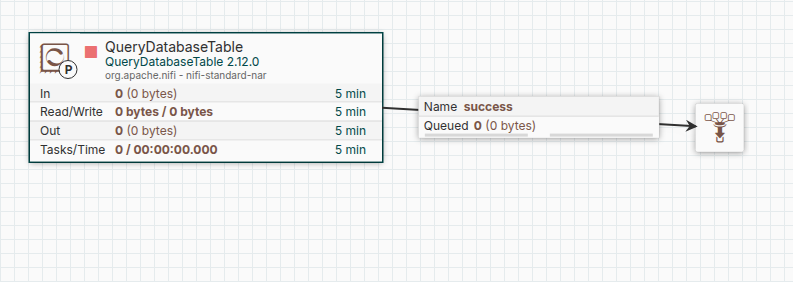
\includegraphics[width=0.8\textwidth]{121.png}
    \caption{Imagen 1}
    \label{fig:imagen1}
\end{figure}
\subsection{Comprobamos el acceso a la tabla de ventas}
\begin{figure}[ht]
    \centering
    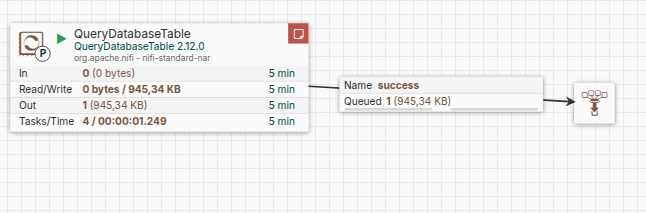
\includegraphics[width=0.8\textwidth]{122.png}
    \caption{Imagen 1}
    \label{fig:imagen1}
\end{figure}
\begin{figure}[ht]
    \centering
    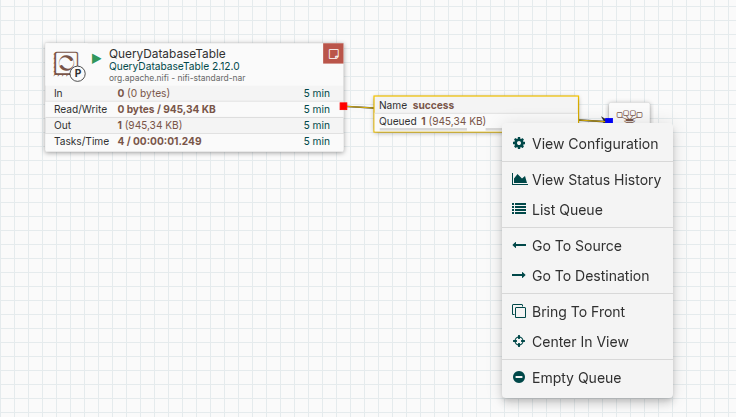
\includegraphics[width=0.8\textwidth]{123.png}
    \caption{Imagen 1}
    \label{fig:imagen1}
\end{figure}
\begin{figure}[ht]
    \centering
    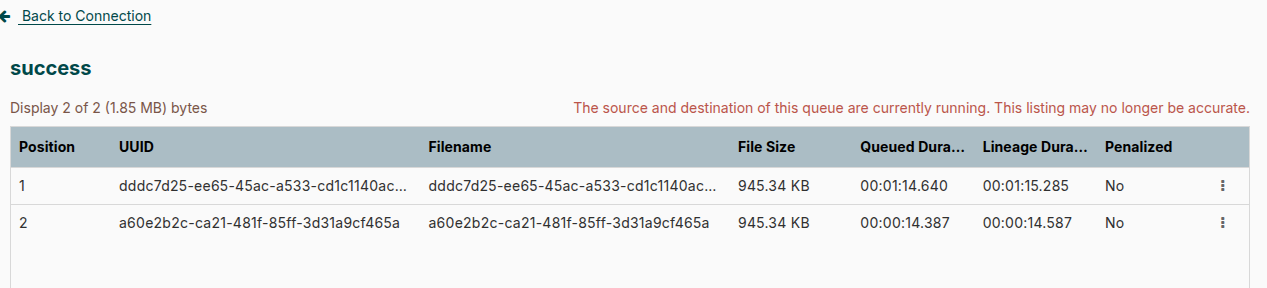
\includegraphics[width=0.8\textwidth]{124.png}
    \caption{Imagen 1}
    \label{fig:imagen1}
\end{figure}
\begin{figure}[ht]
    \centering
    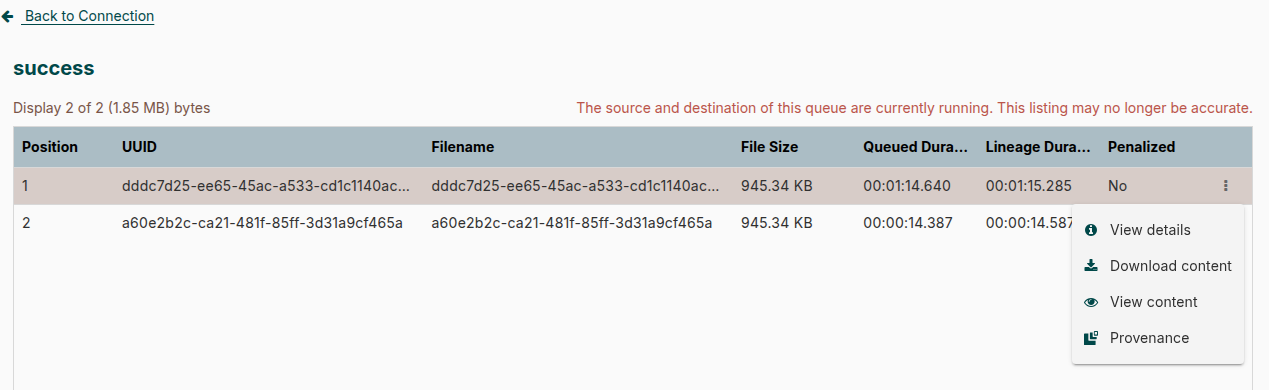
\includegraphics[width=0.8\textwidth]{125.png}
    \caption{Imagen 125}
    \label{fig:imagen125}
\end{figure}
\begin{figure}[ht]
    \centering
    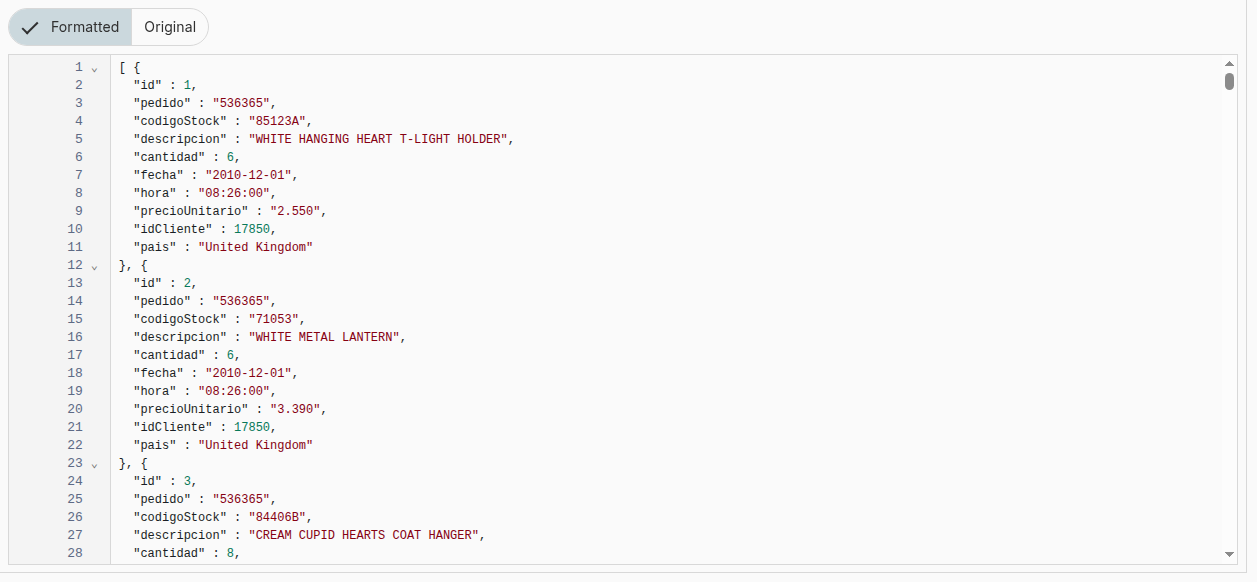
\includegraphics[width=0.8\textwidth]{126.png}
    \caption{Imagen 1}
    \label{fig:imagen1}
\end{figure}
\subsection{Una subsección}
\subsection{Una subsección}
\section{Practica 7 - Practicando la ingesta de datos en Streaming}
\subsection{Una subsección}
\subsection{Una subsección}
\subsection{Una subsección}
\subsection{Una subsección}
\subsection{Una subsección}
\subsection{Una subsección}

\end{document}
